\documentclass[11pt,a4paper]{article}
% Shared preamble for the revision guide and the study plan
\usepackage[margin=20mm,headheight=15pt]{geometry}
\usepackage[T1]{fontenc}\usepackage{lmodern}
\usepackage{amsmath,amssymb,amsthm,mathtools,booktabs,array}
\usepackage[most]{tcolorbox}\usepackage{xcolor,fancyhdr,titlesec,enumitem}
\usepackage{tikz}\usetikzlibrary{arrows.meta,positioning,calc}
\usepackage{hyperref}
\definecolor{navy}{HTML}{18365A}\definecolor{teal}{HTML}{007F88}\definecolor{violet}{HTML}{6E49A3}
\definecolor{orange}{HTML}{C36D16}\definecolor{green}{HTML}{218158}\definecolor{redx}{HTML}{B63A42}
\definecolor{grey}{HTML}{555555}
\hypersetup{colorlinks=true,linkcolor=navy,urlcolor=teal}
\pagestyle{fancy}\fancyhf{}
\fancyhead[L]{\textbf{MATH6342} Linear Systems}\fancyhead[R]{Step-by-step exam revision guide}
\fancyfoot[C]{\thepage}
\titleformat{\section}{\Large\bfseries\color{navy}}{\thesection}{.6em}{}[\titlerule]
\titleformat{\subsection}{\large\bfseries\color{teal}}{\thesubsection}{.5em}{}
\titleformat{\subsubsection}{\normalsize\bfseries\color{violet}}{\thesubsubsection}{.5em}{}
\setlist{topsep=3pt,itemsep=2pt}
\setlength{\parindent}{0pt}\setlength{\parskip}{5pt}
\tcbset{enhanced,breakable,arc=1.5mm,boxrule=.6pt,left=2.5mm,right=2.5mm,top=1.5mm,bottom=1.5mm,
  before skip=6pt,after skip=7pt,fonttitle=\bfseries}
\newtcolorbox{defbox}[1][]{colback=teal!4,colframe=teal,title={Definition / key idea},#1}
\newtcolorbox{thmbox}[1][]{colback=violet!4,colframe=violet,title={Result to know},#1}
\newtcolorbox{methodbox}[1][]{colback=navy!4,colframe=navy,title={Method (step by step)},#1}
\newtcolorbox{workbox}[1][]{colback=orange!5,colframe=orange,title={Worked example},#1}
\newtcolorbox{exambox}[1][]{colback=green!5,colframe=green,title={Exam tip},#1}
\newtcolorbox{warnbox}[1][]{colback=redx!4,colframe=redx,title={Common mistake},#1}
\newtcolorbox{proofbox}[1][]{colback=grey!4,colframe=grey,title={Proof you should be able to write},#1}
\newtcolorbox{qbox}[1][]{colback=white,colframe=navy,title={Exam-style question},#1}
\newtcolorbox{solbox}[1][]{colback=green!3,colframe=green!60!black,title={Full solution},#1}
\newcommand{\Lap}{\mathcal{L}}\newcommand{\CC}{\mathbb{C}}\newcommand{\RR}{\mathbb{R}}
\newcommand{\adj}{\operatorname{adj}}\newcommand{\tr}{\operatorname{trace}}
\newcommand{\rank}{\operatorname{rank}}
\renewcommand{\Re}{\operatorname{Re}}\renewcommand{\Im}{\operatorname{Im}}
\newcommand{\fr}[1]{{\small[frame #1]}}

\begin{document}

\begin{center}
{\Huge\bfseries\color{navy}MATH6342 Linear Systems}\\[6pt]
{\Large Complete step-by-step exam revision guide}\\[6pt]
{\color{teal}Lancaster University 2026/27 \textbullet{} built on Gordon Blower's lecture notes and beamer (frames 1--227)\\
and Assessed Exercises 1--3}
\end{center}

\begin{defbox}[title={How this guide is built, and how to use it}]
\begin{itemize}
\item \textbf{Source of truth.} Every definition, theorem and notation follows the official lecture notes.
Frame numbers are given like this \fr{65} so you can look things up in the beamer.
\item \textbf{Past papers.} No past exam papers were in your uploaded files. The exam-style questions here are
modelled on the lecture examples and on the three Assessed Exercises (AE1--AE3), which show the lecturer's style.
When you get past papers, use Section~\ref{sec:map} to match each question to a method in this guide.
\item \textbf{Every answer checked.} All the worked numbers were checked independently with a computer algebra system.
\item \textbf{New to a topic?} Every subchapter starts with a yellow \textbf{In plain words} box: the idea in everyday language and what the exam question looks like. Read it first, then the formal boxes. Unfamiliar symbol? See the \textbf{decoder} in Section~\ref{sec:decoder}. Before each chapter's exam questions, a \textbf{How to set out a full-mark answer} box shows the layout examiners reward.
\item \textbf{How to revise.} For each chapter: (1) read the \emph{Big picture}; (2) learn the boxed results;
(3) cover the solution and do each worked example yourself; (4) do the exam-style questions at the end of the chapter;
(5) finish with the mock paper in Section~\ref{sec:mock}.
\item \textbf{One afternoon (14:50--19:20)?} Follow the timed study plan in Section~\ref{sec:plan} (also printed separately as \texttt{MATH6342\_Study\_Plan\_1450-1920.pdf}).
\end{itemize}
\end{defbox}

\tableofcontents
\newpage

\section{The whole module on one page}\label{sec:map}

\subsection{The big picture: one story, five chapters}
The whole module is about one object, the \textbf{$(A,B,C,D)$ linear system}
\[
\boxed{\;\frac{dX}{dt}=AX+BU,\qquad Y=CX+DU\;}
\]
with input $U(t)$, state $X(t)$ and output $Y(t)$. Every chapter looks at it from a different angle:

\begin{center}
\renewcommand{\arraystretch}{1.3}
\begin{tabular}{@{}p{3.3cm}p{5.6cm}p{6.2cm}@{}}
\toprule
\textbf{Chapter} & \textbf{Question it answers} & \textbf{Main tools}\\\midrule
1. Description \fr{6--30} & How do I write a machine or an ODE as a system? & block diagrams, reduction of order, companion matrix\\
2. Matrix theory \fr{31--85} & How do I \emph{solve} the system? & $\det$, eigenvalues, $\exp(tA)$, solution formula, $T(s)=D+C(sI-A)^{-1}B$, realisation\\
3. Laplace \fr{86--134} & How do I turn calculus into algebra? & table, properties, convolution, partial fractions, Jordan form\\
4. Transfer functions \& stability \fr{135--161} & Does the output blow up? How does it respond to frequency $\omega$? & gain, phase, Nyquist plot, exponential/marginal/BIBO stability\\
5. Feedback control \fr{162--218} & How do I \emph{make} a system stable? & stable polynomials, $\mathcal S$, Nyquist criterion, PID, coprime factorisation, Youla, Lyapunov, Sylvester\\
\bottomrule
\end{tabular}
\end{center}

\subsection{The ``chain'' you must be able to travel along}
\begin{center}
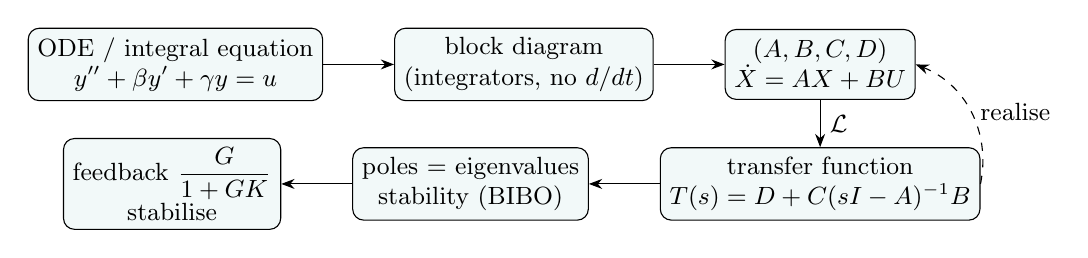
\begin{tikzpicture}[node distance=6mm and 9mm, every node/.style={draw,rounded corners,align=center,font=\small,fill=teal!5}]
\node (ode) {ODE / integral equation\\ $y''+\beta y'+\gamma y=u$};
\node (bd) [right=of ode] {block diagram\\(integrators, no $d/dt$)};
\node (abcd) [right=of bd] {$(A,B,C,D)$\\$\dot X=AX+BU$};
\node (T) [below=of abcd] {transfer function\\$T(s)=D+C(sI-A)^{-1}B$};
\node (st) [left=of T] {poles $=$ eigenvalues\\ stability (BIBO)};
\node (fb) [left=of st] {feedback $\dfrac{G}{1+GK}$\\ stabilise};
\draw[-Stealth] (ode)--(bd); \draw[-Stealth] (bd)--(abcd); \draw[-Stealth] (abcd)--node[draw=none,fill=none,right]{$\Lap$}(T);
\draw[-Stealth] (T)--(st); \draw[-Stealth] (st)--(fb);
\draw[-Stealth,dashed] (T.east) to[bend right=40] node[draw=none,fill=none,right]{realise} (abcd.east);
\end{tikzpicture}
\end{center}

\subsection{Question-type finder (use this in the exam)}
\begin{center}
\renewcommand{\arraystretch}{1.25}
\begin{tabular}{@{}p{7.3cm}p{8cm}@{}}
\toprule
\textbf{If the question says\dots} & \textbf{Go to / do this}\\\midrule
``Express as a block diagram (no differentiators)'' & Integrate both sides until no derivatives are left; \S\ref{sec:bd}\\
``Write in matrix form $(A,B,C,D)$'' / ``introduce state $v=dx/dt$'' & Reduction of order, \S\ref{sec:reduction}\\
``Find a matrix with characteristic polynomial $p$'' & Companion matrix, \S\ref{sec:companion}\\
``Find $(sI-A)^{-1}$'' & Adjugate / triangular trick, \S\ref{sec:resolvent}\\
``Find $\exp(tA)$'' & Diagonalise, Jordan or inverse Laplace of $(sI-A)^{-1}$, \S\ref{sec:exp}\\
``Solve $\dot X=AX+BU$, $X(0)=X_0$'' & Variation of constants, \S\ref{sec:solution}\\
``Compute the transfer function'' & $T(s)=D+C(sI-A)^{-1}B$, \S\ref{sec:tf}\\
``Realise $T(s)$ as a SISO'' & Companion realisation, \S\ref{sec:realise}\\
``Rank of $[C;CA;\dots;CA^{n-1}]$'' & \S\ref{sec:rank}\\
``Laplace transform of \dots{} from the definition'' & Integrate by parts / exponential trick, \S\ref{sec:lapdef}\\
``Solve the IVP/integral equation by Laplace'' & \S\ref{sec:ivp}, \S\ref{sec:conv}\\
``Jordan form, minimal polynomial, multiplicities'' & \S\ref{sec:jordan}\\
``Gain and phase / Bode / Nyquist'' & \S\ref{sec:freq}\\
``Is the system stable / BIBO stable?'' & Eigenvalues of $A$ / poles of $T$, \S\ref{sec:stab}\\
``Is the polynomial stable?'' / ``for which $k$ is it stable?'' & \S\ref{sec:stabpoly}\\
``Find a controller $-a-b/s$ / PID that stabilises $G$'' & \S\ref{sec:pid}\\
``Coprime factorisation / stabilising controller'' & \S\ref{sec:coprime}\\
``Internally stable / well-posed'' & \S\ref{sec:internal}\\
``Positive definite / Lyapunov / Sylvester'' & \S\ref{sec:posdef}--\S\ref{sec:sylv}\\
``Prove that \dots'' & the grey \emph{Proof} boxes; list in \S\ref{sec:proofs}\\
\bottomrule
\end{tabular}
\end{center}

\begin{exambox}[title={Exam technique for this module}]
\begin{enumerate}
\item \textbf{State the formula first}, then substitute. E.g.\ write ``$T(s)=D+C(sI-A)^{-1}B$'' before doing any algebra. This earns method marks even if the arithmetic slips.
\item \textbf{Keep track of shapes.} $A$ is $n\times n$, $B$ is $n\times k$, $C$ is $m\times n$, $D$ is $m\times k$. If shapes do not match, you have made an error.
\item \textbf{Check your answer cheaply:} $\det$ = product of eigenvalues, $\tr$ = sum of eigenvalues; put $t=0$ into $\exp(tA)$ (should give $I$); put $s\to\infty$ into $T(s)$ (should give $D$); put $t=0$ into an IVP solution.
\item \textbf{Use the lecture notes' sign conventions}: $\chi_A(s)=\det(sI-A)$ (not $\det(A-sI)$); the adjoint $A'$ is the conjugate transpose; LHP is the \emph{open} left half plane.
\item \textbf{Say why}: ``all poles have negative real part, hence $T\in\mathcal S$'' is a full-mark sentence; ``it is stable'' is not.
\end{enumerate}
\end{exambox}
\newpage

\section{Symbol and word decoder}\label{sec:decoder}
Most confusion in this module comes from notation, not ideas. Keep this page open while you revise.

\subsection*{Letters and symbols}
\begin{center}
\renewcommand{\arraystretch}{1.35}
\small
\begin{tabular}{@{}p{3.2cm}p{12cm}@{}}
\toprule
\textbf{Symbol} & \textbf{What it means, in words}\\\midrule
$t$ & time ($t>0$)\\
$u(t)$, $U(t)$ & the \textbf{input}: what we feed in (a force, a voltage, \dots); capital $U$ when it is a vector\\
$y(t)$, $Y(t)$ & the \textbf{output}: what we measure\\
$x(t)$, $X(t)$ & the \textbf{state}: the internal variables (e.g.\ position and velocity)\\
$\dot X$, $X'$, $\frac{dX}{dt}$ & all mean the derivative with respect to time\\
$\int^{(n)}$ & integrate $n$ times, each time from $0$\\
$A,B,C,D$ & state, input, output and straight-through matrices of the system $\dot X=AX+BU$, $Y=CX+DU$\\
$n,k,m$ & number of states, inputs, outputs\\
$I$ & identity matrix\\
$A^\top$ & transpose (swap rows and columns)\\
$A'$ & \textbf{adjoint}: transpose \emph{and} complex conjugate (equals $A^\top$ for real $A$). \emph{Not} a derivative!\\
$\adj(A)$ & adjugate: transpose of the matrix of cofactors; $A^{-1}=\adj(A)/\det A$\\
$\chi_A(s)$ & characteristic polynomial $\det(sI-A)$; its roots are the eigenvalues\\
$\lambda$ & usually an eigenvalue (in \S\ref{sec:coprime} also the new variable $\frac1{1+s}$)\\
$\exp(tA)$ & the matrix exponential $I+tA+\frac{t^2A^2}{2!}+\cdots$ (MATLAB \texttt{expm})\\
$(sI-A)^{-1}$ & the resolvent; the Laplace transform of $\exp(tA)$\\
$s$ & the Laplace variable (a complex number); think ``$s$ replaces $d/dt$''\\
$\hat f(s)$, $\Lap(f)(s)$ & the Laplace transform of $f$\\
$f*g$ & Laplace convolution $\int_0^tf(t-u)g(u)\,du$\\
$H(t-b)$, $\delta_b$ & step that switches on at $t=b$; unit impulse at $t=b$\\
$T(s)$ & transfer function: output $=T(s)\times$input in the $s$-world\\
$\omega$ & angular frequency (rad/s); we put $s=i\omega$ to study pure tones\\
$\Gamma(\omega)$, $\phi(\omega)$ & gain $|T(i\omega)|$ and phase $\arg T(i\omega)$\\
$\Re\lambda$ & real part of $\lambda$; its sign decides growth or decay of $e^{\lambda t}$\\
LHP, RHP & open left half plane $\{\Re s<0\}$ (``safe''), open right half plane $\{\Re s>0\}$\\
$\mathcal S$ & stable rational functions: proper, and all poles in the LHP\\
$G$, $K$ & plant (the machine being controlled) and controller\\
$J_k(\lambda)$ & $k\times k$ Jordan block\\
$\langle z,w\rangle$, $\|z\|$ & inner product $\sum z_j\bar w_j$ and length\\
\bottomrule
\end{tabular}
\end{center}

\subsection*{Words}
\begin{center}
\renewcommand{\arraystretch}{1.35}
\small
\begin{tabular}{@{}p{3.6cm}p{11.6cm}@{}}
\toprule
\textbf{Word} & \textbf{Plain meaning}\\\midrule
SISO / MIMO & one input and one output / several inputs and outputs\\
open loop / feedback & no signal comes back / output is fed back into the input\\
proper / strictly proper & $\deg(\text{top})\le\deg(\text{bottom})$ / $<$; i.e.\ $T(s)$ tends to a constant / to $0$ as $s\to\infty$\\
pole / zero & where the denominator / numerator of $T(s)$ is zero\\
realisation & building $(A,B,C,D)$ that has a given $T(s)$\\
companion matrix & the standard matrix with a given characteristic polynomial (ones above the diagonal, coefficients in the last row)\\
complementary function / particular integral & solution with no input / extra part caused by the input\\
exponentially stable & every solution decays to 0 like $e^{-\delta t}$ (all $\Re\lambda<0$)\\
marginally stable & every solution stays bounded but need not decay (eigenvalues on the axis, $1\times1$ blocks)\\
BIBO stable & every bounded input gives a bounded output\\
resonance & bounded input at the natural frequency gives an unbounded output\\
Nyquist plot & the curve traced by $T(i\omega)$ in the complex plane\\
Bode plot & gain (in dB) and phase against $\omega$ on a log scale\\
coprime & $P,Q$ have no common factor: $PX+QY=1$ for some $X,Y$\\
internally stable & every signal inside the feedback loop stays bounded\\
positive definite & matrix version of ``positive'': $\langle Kz,z\rangle>0$ for $z\neq0$\\
\bottomrule
\end{tabular}
\end{center}

\subsection*{Six facts that unlock the whole module}
\begin{enumerate}
\item The \textbf{eigenvalues of $A$} decide everything: each gives a term $e^{\lambda t}$ in the solution.
\item $\Re\lambda<0$ means decay (good), $\Re\lambda>0$ means growth (bad), $\Re\lambda=0$ is the borderline.
\item The \textbf{poles of $T(s)$} are eigenvalues of $A$, so you can read stability from $T(s)$.
\item \textbf{Laplace} turns $\frac{d}{dt}$ into ``$\times s$'' and $\int_0^t$ into ``$\div s$''.
\item \textbf{Feedback} changes the denominator: $T=\frac{G}{1+GK}$, so choosing $K$ moves the poles.
\item A polynomial is stable iff its roots are in the LHP; quick necessary test: all coefficients positive.
\end{enumerate}
\newpage

% Study plan 14:30-19:00, subchapter by subchapter. GENERATED by gen_plan.py: edit there.
\providecommand{\G}[1]{\S\ref{#1}, p.\,\pageref{#1}}
\providecommand{\tick}{$\square$}
\newtcolorbox{chapplan}[1]{colback=white,colframe=navy,title={#1},left=2mm,right=2mm}
\newcommand{\sub}[5]{\par\smallskip\noindent\textbf{\color{navy}#1}\ \ {\small(#2 min)}\ \ \textbf{#4} \hfill{\small\color{grey}\G{#3}}\par
 \noindent\hspace*{4mm}\parbox{\dimexpr\linewidth-4mm}{\textbf{Do:} #5}\par}
\newcommand{\gate}[1]{\noindent\hspace*{4mm}\parbox{\dimexpr\linewidth-4mm}{\tick\ \textbf{Move on when you can} #1}\par\smallskip}
\newcommand{\pausebox}[2]{\begin{tcolorbox}[colback=green!6,colframe=green!60!black,title={Break \quad #1}]#2\end{tcolorbox}}

\section{Your study plan: 14:30 to 19:00, subchapter by subchapter}\label{sec:plan}

\subsection*{How it works}
You go through the guide \textbf{one subchapter at a time}, in order. Each subchapter has a time slot, a \textbf{Do} list and a
\textbf{Move on when you can\dots} test. Only move to the next subchapter when you can pass its test \emph{without looking}.

\begin{methodbox}[title={The loop for every subchapter}]
\begin{enumerate}
\item \textbf{Read} the definition and method boxes slowly. For every step ask ``\emph{why} is this allowed?''
\item \textbf{Cover} each worked example and do it yourself on paper; uncover one line only when stuck.
\item \textbf{Explain} the main idea aloud in one or two sentences, as if to a friend.
\item \textbf{Test}: close the guide and do the ``Move on when you can'' task. Pass $\Rightarrow$ tick the box and move on.
\end{enumerate}
\end{methodbox}
\begin{warnbox}[title={The stuck rule (keeps you on time without skipping understanding)}]
If you still cannot pass a test \textbf{3 minutes after its slot ends}, write the subchapter number on a ``come back'' list, put a star next to it, and move on.
Later subchapters often make earlier ones click. The final slot (18:50--19:00) is reserved for your starred subchapters.
Never just reread: always \emph{do} something (write, derive, explain aloud).
\end{warnbox}
Have ready: the guide, plain paper, pen, calculator, a ``come back'' list, phone in another room.

\subsection*{Timetable at a glance}
\begin{center}\renewcommand{\arraystretch}{1.25}\small
\begin{tabular}{@{}p{2.3cm}p{1cm}p{7.5cm}p{3.4cm}@{}}\toprule
\textbf{Time} & \textbf{Min} & \textbf{Part} & \textbf{Guide}\\\midrule
14:30--14:35 & 5 & Overview & \G{sec:map}\\
14:35--15:11 & 36 & Chapter 1: Describing linear systems & \G{ch1}\\
15:11--15:16 & 5 & Break & \\
15:16--16:22 & 66 & Chapter 2: Matrix theory & \G{ch2}\\
16:22--16:32 & 10 & Break & \\
16:32--17:20 & 48 & Chapter 3: Laplace transforms & \G{ch3}\\
17:20--17:25 & 5 & Break & \\
17:25--17:55 & 30 & Chapter 4: Frequency response and stability & \G{ch4}\\
17:55--18:00 & 5 & Break & \\
18:00--18:50 & 50 & Chapter 5: Feedback control & \G{ch5}\\
18:50--19:00 & 10 & Come-back list and recall & \G{sec:proofs}\\
\bottomrule\end{tabular}\end{center}
Each chapter is split into its subchapters on the following pages, with the minutes chosen by how hard and how examinable each one is.
\subsection*{Subchapter by subchapter}
\begin{chapplan}{Start \quad 14:30--14:35 \quad The whole module on one page}
\sub{14:30--14:35}{5}{sec:map}{The big picture}{Read the chapter table and the chain diagram. Then, closed book, write the chain ODE $\to$ diagram $\to$ $(A,B,C,D)$ $\to$ $T(s)$ $\to$ stability $\to$ feedback.}
\gate{write $\dot X=AX+BU$, $Y=CX+DU$ and $T(s)=D+C(sI-A)^{-1}B$ from memory.}
\end{chapplan}
\begin{chapplan}{Chapter 1: Describing linear systems \quad 14:35--15:11 (36 min)}
\sub{14:35--14:39}{4}{ss:1-1}{Linear operators and the five building blocks}{Read the definition box. Say what each block does to a signal $u$. Do the exam tip: show $Lf=tf''+3\int_0^tf$ is linear.}
\gate{say what a tap, summing junction, integrator, differentiator and amplifier do, and check linearity of a given $L$.}
\sub{14:39--14:44}{5}{ss:1-2}{Block diagrams: open loop and feedback}{Cover and redo Black's amplifier ($y=u+\theta y\Rightarrow y=u/(1-\theta)$) and the cyclist ($v=-\frac km\int v+\frac1m\int u$).}
\gate{tell open loop from feedback, and write the equation at a summing junction.}
\sub{14:44--14:54}{10}{ss:1-3}{How to turn an equation into a block diagram}{Learn the 5-step method box. Cover and redo A1.1(i), A1.1(ii) (integrate twice, solve for $y$, nest the integrals) and A1.2.}
\gate{turn $y''+4y=u'$ (or similar) into a diagram with \emph{no differentiators}, closed book.}
\sub{14:54--15:00}{6}{ss:1-4}{Reduction of order and the matrix form}{Learn the 4-step method. Cover and redo A1.3 ($m\ddot x+kx=u$) and the damped oscillator.}
\gate{write $A,B,C,D$ for any $n$-th order constant-coefficient ODE (remember to make it monic first).}
\sub{15:00--15:05}{5}{ss:1-5}{The companion matrix}{Learn the sign/order rule (last row $-a_0,\dots,-a_{n-1}$). Redo A2.2. Read the induction proof once.}
\gate{write a matrix with characteristic polynomial $s^3-2s^2+s+7$ in 30 seconds.}
\sub{15:05--15:11}{6}{ss:1-6}{Exam-style questions for Chapter 1}{Do Q1.1 and Q1.2 closed book, then mark against the solutions. Q1.3 if time.}
\gate{get Q1.1 and Q1.2 fully right.}
\end{chapplan}
\pausebox{15:11--15:16}{Stand up, get water, no phone.}
\begin{chapplan}{Chapter 2: Matrix theory \quad 15:16--16:22 (66 min)}
\noindent\textbf{Warm-up recall (inside the first slot, 1 min, closed book):} $A,B,C,D$ for $m\ddot x+kx=u$; the companion matrix of $s^3+2s+5$.\par
\sub{15:16--15:20}{4}{ss:2-1}{Determinants, cofactors, characteristic polynomial}{Read the box. Note: $\chi_A(s)=\det(sI-A)$, adjugate $=$ \emph{transpose} of cofactors, $2\times2$: $s^2-\tr A\,s+\det A$.}
\gate{write $\chi_A$ for a $2\times2$ matrix instantly and explain what the adjugate is.}
\sub{15:20--15:27}{7}{ss:2-2}{Computing the resolvent $(sI-A)^{-1}$}{Learn the 5-step method. Cover and redo A1.4 (upper triangular, so many cofactors are 0).}
\gate{compute $(sI-A)^{-1}$ for a $2\times2$ matrix in under 3 minutes and check it.}
\sub{15:27--15:30}{3}{ss:2-3}{Norms and Cauchy--Schwarz}{Read the results box and the Cauchy--Schwarz proof once (discriminant $\le0$ idea).}
\gate{state $\|AB\|\le\|A\|\|B\|$ and the one-line idea of the Cauchy--Schwarz proof.}
\sub{15:30--15:34}{4}{ss:2-4}{Rank and the matrices $Q$, $R$ (AE2)}{Redo A2.3(i)--(ii). Read the ``why rank matters'' box (rank drop $\leftrightarrow$ pole cancels).}
\gate{prove $Q^\top=R$ and find $R$ when $C^\top$ is an eigenvector of $A^\top$.}
\sub{15:34--15:40}{6}{ss:2-5}{Eigenvalues, diagonalisation, Cayley--Hamilton}{Read the results box and the $AS=S\Delta$ proof. Cover and redo the Cayley--Hamilton example ($A^{-1}$ and $A^3$).}
\gate{explain why $g(A)=Sg(\Delta)S^{-1}$ and use Cayley--Hamilton to invert a $2\times2$.}
\sub{15:40--15:53}{13}{ss:2-6}{The matrix exponential}{Learn the 3-way method box. Cover and redo: distinct eigenvalues, repeated eigenvalue ($e^{\lambda t}(I+t(A-\lambda I))$), $\pm i$ (rotation). Check $t=0$ every time. Read A3.3.}
\gate{compute $\exp(tA)$ for a $2\times2$ with distinct \emph{and} with repeated eigenvalues, and check it.}
\sub{15:53--16:00}{7}{ss:2-7}{The solution formula for $\dot X=AX+BU$}{Say the integrating-factor proof aloud. Cover and redo the step-response example; check $y(\infty)=T(0)$.}
\gate{write $X(t)=\exp(tA)X_0+\int_0^t\exp((t-s)A)BU(s)\,ds$ and explain each term (CF and PI).}
\sub{16:00--16:02}{2}{ss:2-8}{SISO and MIMO $(A,B,C,D)$}{Read the box: names and shapes of $A,B,C,D$.}
\gate{give the shapes of $A,B,C,D$ for $k$ inputs, $n$ states and $m$ outputs.}
\sub{16:02--16:09}{7}{ss:2-9}{Rational functions and the transfer function}{Learn proper/strictly proper, poles/zeros, $T=D+C(sI-A)^{-1}B$. Redo the damped-oscillator example; read A2.1 and the proof of Prop 0.20.}
\gate{compute $T(s)$ for a $2\times2$ system and say why every pole is an eigenvalue (but not conversely).}
\sub{16:09--16:17}{8}{ss:2-10}{Realisation: from $T(s)$ back to $(A,B,C,D)$}{Learn the 4-step method. Cover and redo the frame 79 example and the proper example with long division.}
\gate{realise any proper $T(s)$ (including the $D\neq0$ case) and check it by the determinant formula.}
\sub{16:17--16:22}{5}{ss:2-11}{Exam-style questions for Chapter 2}{Do Q2.1 closed book and mark it. Q2.2 if time.}
\gate{get Q2.1 fully right.}
\end{chapplan}
\pausebox{16:22--16:32}{Longer break: eat something. You are halfway.}
\begin{chapplan}{Chapter 3: Laplace transforms \quad 16:32--17:20 (48 min)}
\noindent\textbf{Warm-up recall (inside the first slot, 1 min, closed book):} the solution formula for $\dot X=AX+BU$; $\exp(tA)$ for a double eigenvalue; $T(s)$.\par
\sub{16:32--16:36}{4}{ss:3-1}{Definition and the table}{Read the definition. Cover the table and write it from memory twice.}
\gate{write the whole table from memory.}
\sub{16:36--16:40}{4}{ss:3-2}{Properties}{Learn the 6 properties; say the derivative-rule proof aloud (integration by parts).}
\gate{state $\Lap(f')$, $\Lap(f'')$, the shift rule and the $t f(t)$ rule.}
\sub{16:40--16:45}{5}{ss:3-3}{Laplace transforms from the definition}{Cover and redo A3.1 ($\cos2\omega t$ via $e^{\pm2i\omega t}$, then $\sin^2\omega t$). Read the $x^2$ example.}
\gate{find $\Lap(e^{at})$ and $\Lap(\cos at)$ from the definition, stating the condition on $s$.}
\sub{16:45--16:50}{5}{ss:3-4}{Partial fractions and inverting}{Learn the 5-step invert method and Lerch. Cover and redo the repeated-pole example.}
\gate{invert a function with a repeated pole and one with an irreducible quadratic (complete the square).}
\sub{16:50--16:59}{9}{ss:3-5}{Solving initial value problems}{Learn the 5-step IVP method. Cover and redo A3.2 and the second-order step example.}
\gate{solve a second-order IVP by Laplace from start to finish, including the check.}
\sub{16:59--17:04}{5}{ss:3-6}{Convolution and integral equations}{Learn $\Lap(f*g)=\hat f\hat g$; read the proof. Cover and redo $y=t+\int_0^t\sin(t-u)y(u)\,du$.}
\gate{spot a convolution in an integral equation and solve it.}
\sub{17:04--17:09}{5}{ss:3-7}{Laplace transform of $(A,B,C,D)$}{Derive $\hat Y=T\hat U+C(sI-A)^{-1}X(0)$ yourself. Read the complex-eigenvalue $\exp(tA)$ example.}
\gate{explain why $\hat Y=T(s)\hat U$ when $X(0)=0$, and get $\exp(tA)$ as $\Lap^{-1}[(sI-A)^{-1}]$.}
\sub{17:09--17:15}{6}{ss:3-8}{Jordan canonical form}{Learn: algebraic mult.\ = total block size; geometric mult.\ = number of blocks; minimal polynomial uses the largest block. Read the corrected frame 119 example.}
\gate{read off multiplicities and the minimal polynomial from a Jordan form, and find $\exp(tJ_2(\lambda))$.}
\sub{17:15--17:20}{5}{ss:3-9}{Exam-style questions for Chapter 3}{Do Q3.2 and Q3.4 closed book and mark them.}
\gate{get Q3.2 and Q3.4 fully right.}
\end{chapplan}
\pausebox{17:20--17:25}{Short break.}
\begin{chapplan}{Chapter 4: Frequency response and stability \quad 17:25--17:55 (30 min)}
\noindent\textbf{Warm-up recall (inside the first slot, 1 min, closed book):} $\Lap(f')$, $\Lap(f'')$, $\Lap(\sin at)$, $\Lap(f*g)$.\par
\sub{17:25--17:27}{2}{ss:4-1}{Transfer functions and realisation}{Read the box (Theorems 0.38 and 0.46).}
\gate{state what can be realised by a SISO, and by a BIBO-stable SISO.}
\sub{17:27--17:35}{8}{ss:4-2}{Frequency response, gain and phase}{Learn the method and the quadrant warning. Cover and redo $\frac1{s+1}$ including its Nyquist circle; read the $\frac1{as^2+bs+1}$ example.}
\gate{find $\Gamma(\omega)$, $\phi(\omega)$ for a simple $T$ and sketch its Nyquist plot.}
\sub{17:35--17:41}{6}{ss:4-3}{Stability: the three cases}{Learn the three-row table and the method. Go through the five worked examples and say why each is classified that way.}
\gate{classify $\dot X=AX$ as exponentially stable, marginal or unstable, including the Jordan-block case.}
\sub{17:41--17:44}{3}{ss:4-4}{The damped harmonic oscillator}{Read the table. Connect it to ``$s^2+\beta s+\gamma$ stable iff $\beta,\gamma>0$''.}
\gate{say for which $\beta,\gamma$ the oscillator is stable, marginal or unstable.}
\sub{17:44--17:47}{3}{ss:4-5}{Resonance}{Read the undamped oscillator example. Understand the double pole $\Rightarrow$ $t\sin\nu t$.}
\gate{explain in two sentences why marginally stable is \emph{not} BIBO stable.}
\sub{17:47--17:52}{5}{ss:4-6}{BIBO stability theorems}{Say the proof of Theorem 0.42 aloud (bound $\|\exp(tA)\|\le Me^{-\delta t}$, integrate). Read the outline of Theorem 0.45.}
\gate{write the proof of Theorem 0.42 closed book.}
\sub{17:52--17:55}{3}{ss:4-7}{Exam-style questions for Chapter 4}{Do Q4.1 closed book and mark it.}
\gate{get Q4.1 fully right.}
\end{chapplan}
\pausebox{17:55--18:00}{Short break. Last chapter next.}
\begin{chapplan}{Chapter 5: Feedback control \quad 18:00--18:50 (50 min)}
\noindent\textbf{Warm-up recall (inside the first slot, 1 min, closed book):} the stability table for $\dot X=AX$; the definition of BIBO.\par
\sub{18:00--18:05}{5}{ss:5-1}{Stable polynomials}{Learn Prop 0.43 and its proof, the counterexample $(s+1)(s^2+1)$, and the degree 2 and 3 tests.}
\gate{decide whether a polynomial of degree $\le3$ is stable, and prove Prop 0.43.}
\sub{18:05--18:08}{3}{ss:5-2}{The ring $\mathcal S$}{Learn the two conditions (proper, poles in open LHP) and why $\mathcal S$ is not a field.}
\gate{say whether $\frac{s^2}{s+1}$, $\frac{1}{s^2+1}$, $\frac{s}{(s+1)^2}$ are in $\mathcal S$, with reasons.}
\sub{18:08--18:13}{5}{ss:5-3}{Nyquist's criterion}{Learn the statement and $N=Z-P$. Cover and redo the $\frac{k}{(s+1)^3}$ example (crossing at $-k/8$).}
\gate{find the gain range for stability from where the Nyquist plot crosses the negative real axis.}
\sub{18:13--18:19}{6}{ss:5-4}{The simple feedback loop and PID}{Derive $T=G/(1+GK)$ from the diagram. Cover and redo the PI example and the proportional example.}
\gate{find a PI or PD controller that stabilises a simple plant, stating your sign convention.}
\sub{18:19--18:23}{4}{ss:5-5}{Euclid, B\'ezout and matrix completion}{Learn the algorithm. Cover and redo worked examples (a) and (b); read (c) and (d).}
\gate{find $M,N$ with $PM+QN=1$ for two coprime polynomials of low degree.}
\sub{18:23--18:32}{9}{ss:5-6}{Coprime factorisation and Youla}{Learn the 4-step algorithm and the four formulas $QY,PY,XQ,PX$. Cover and redo worked example A ($\frac1{s-1}$); read B.}
\gate{do the whole algorithm for $G=\frac1{s-a}$ and check all four closed-loop functions.}
\sub{18:32--18:36}{4}{ss:5-7}{Well-posedness and internal stability}{Read Lemma 0.51 and the ``trap'' example.}
\gate{explain why all four functions must be in $\mathcal S$, using the trap example.}
\sub{18:36--18:40}{4}{ss:5-8}{Positive definite matrices}{Learn the three equivalent conditions. Cover and redo A3.4 (i)--(v) and the minors example.}
\gate{test a $3\times3$ matrix by leading minors and prove A3.4(iii).}
\sub{18:40--18:44}{4}{ss:5-9}{Lyapunov's criterion and equation}{Say the proof aloud ($V=\langle KX,X\rangle$ is decreasing). Redo the $K=I$ example; read the Lyapunov-equation example.}
\gate{use $K=I$ to show solutions are bounded, and write the proof.}
\sub{18:44--18:46}{2}{ss:5-10}{Sylvester's equation}{Read the result and the $1\times1$ intuition $a\neq-b$.}
\gate{state when $AY+YB=-C$ has a unique solution for every $C$.}
\sub{18:46--18:50}{4}{ss:5-11}{Exam-style questions for Chapter 5}{Do Q5.1 and Q5.3 closed book and mark them.}
\gate{get Q5.1 and Q5.3 fully right.}
\end{chapplan}
\begin{chapplan}{Finish \quad 18:50--19:00 \quad Come-back list and recall}
\sub{18:50--18:57}{7}{sec:proofs}{Your starred subchapters}{Go back to each subchapter on your ``come back'' list and retry its test. If the list is empty, do mock question M2 (\G{sec:mock}).}
\gate{pass the test of at least one starred subchapter.}
\sub{18:57--19:00}{3}{sec:mock}{Formula sheet from memory}{Cover the formula sheet (last page) and write as many lines as you can; mark what you missed.}
\gate{write at least 15 of the 20 formula-sheet lines.}
\end{chapplan}
\subsection*{Come-back list}
\begin{center}\renewcommand{\arraystretch}{1.6}
\begin{tabular}{@{}p{2.5cm}p{8cm}p{3.5cm}@{}}\toprule
\textbf{Subchapter} & \textbf{What I could not do} & \textbf{Fixed? (time)}\\\midrule
 & & \\ & & \\ & & \\ & & \\ & & \\ & & \\\bottomrule\end{tabular}\end{center}
\begin{exambox}[title={Next session}]
Start with 10 minutes writing the formula sheet from memory, then your come-back list, then the proofs list (\G{sec:proofs}) and the full mock paper (\G{sec:mock}).
\end{exambox}
\newpage

\tikzset{blk/.style={draw,minimum height=7mm,minimum width=9mm,fill=white,font=\small},
 sumj/.style={draw,circle,inner sep=1.2pt,font=\scriptsize},
 tap/.style={circle,fill,inner sep=1.3pt},
 ar/.style={-Stealth}}

\section{Chapter 1: Linear systems and their description \texorpdfstring{\fr{6--30}}{}}
\label{ch1}

\subsection*{Big picture}
A \textbf{linear system} is a machine with input $u(t)$, output $y(t)$ and internal \textbf{state} $x(t)$.
The state is ``everything you need to know now, so that together with future inputs you can predict the future''.
In this chapter we learn to \emph{draw} systems (block diagrams) and to \emph{rewrite} any constant-coefficient ODE as a first order
matrix system $\dot X=AX+Bu$. Nothing is solved yet; that is Chapter 2.

\subsection{Linear operators and the five building blocks \texorpdfstring{\fr{7--9}}{}}\label{ss:1-1}
\begin{plainbox}
A linear system is a \textbf{machine}: a signal $u(t)$ goes in, a signal $y(t)$ comes out. Inside, the signal passes through
simple ``boxes''. Each box does one job: \emph{scale it} (amplifier), \emph{add up the history} (integrator), \emph{measure how fast it changes}
(differentiator), \emph{combine signals} (summing junction) or \emph{copy it} (tap).
\textbf{Linear} means ``double the input, double the output; add two inputs, add the outputs''.
\par\smallskip\textbf{In the exam this looks like:} ``Show that $L$ is linear'' or ``which of these maps are linear?''.
\end{plainbox}
\begin{defbox}
$L:V\to W$ is \textbf{linear} if $L(\lambda f+\mu g)=\lambda Lf+\mu Lg$ for all $f,g$ and all $\lambda,\mu\in\CC$.
The basic linear operators (on continuously differentiable $f:[0,\infty)\to\CC$) are
\begin{enumerate}[label=(\roman*)]
\item \textbf{differentiator} $f\mapsto df/dt$, drawn $[d/dt]$;
\item \textbf{integrator} $f\mapsto\int_0^x f(t)\,dt$, drawn $[\int]$ (always integrate from $0$);
\item \textbf{amplifier} $f\mapsto af$ for a constant $a\in\CC$, drawn $[a]$ (called an amplifier even if $|a|<1$);
\item \textbf{multiplication} by a fixed function $h$: $f\mapsto hf$, drawn $[h]$;
\item \textbf{evaluation} $f\mapsto f(t_0)$, drawn $[\delta_{t_0}]$.
\end{enumerate}
Two connectors: a \textbf{summing junction} $\oplus$ adds the incoming signals (with the signs written on the arrows);
a \textbf{tap} $\bullet$ copies a signal onto several wires \emph{without} dividing it (like a point in an electrical circuit,
all wires at a tap carry the same voltage).
\end{defbox}

\begin{warnbox}
A tap does \textbf{not} split the signal into halves. If $u$ goes into a tap with three wires out, each wire carries $u$.
\end{warnbox}

\begin{exambox}
``Show that $L$ is linear'' questions: write out $L(\lambda f+\mu g)$ and use linearity of differentiation/integration.
E.g.\ $Lf=t\,f''+3\int_0^t f$ is linear since $L(\lambda f+\mu g)=t(\lambda f''+\mu g'')+3\int_0^t(\lambda f+\mu g)=\lambda Lf+\mu Lg$.
A map like $f\mapsto f^2$ or $f\mapsto f+1$ is \textbf{not} linear (check $L(2f)\neq 2Lf$, or $L(0)\neq0$).
\end{exambox}

\subsection{Block diagrams: rules, open loop and feedback \texorpdfstring{\fr{11--17}}{}}\label{ss:1-2}
\begin{plainbox}
\textbf{Feedback} means part of the output is sent back to the input. Think of a thermostat: the room temperature (output)
is measured and used to switch the heater (input). \textbf{Negative} feedback calms the system down (going faster creates drag);
\textbf{positive} feedback pushes it further the same way (more birds $\Rightarrow$ more births). Open loop = no signal ever comes back.
\par\smallskip\textbf{In the exam this looks like:} ``Find the output of this feedback diagram'' (write the equation at the summing junction and solve for $y$).
\end{plainbox}
\begin{defbox}
A block diagram is a directed graph from input $u$ to output $y$ built from $u,y,\delta_0,\oplus,\bullet,d/dt,\int,a,h$.
\begin{itemize}
\item $u$ and $y$ have degree one; every other vertex has degree two or three.
\item No loops at a vertex and no multiple edges; every vertex lies on a directed path from $u$ to $y$.
\item If the diagram contains a \textbf{circuit} there is \textbf{feedback} (closed loop); otherwise it is \textbf{open loop} (straight through).
\end{itemize}
\end{defbox}

\begin{workbox}[title={Worked example: Black's amplifier \fr{15} (positive feedback)}]
\begin{center}
\begin{tikzpicture}
\node (u) at (0,0) {$u$};
\node[sumj] (s) at (1.6,0) {$+$};
\node[tap] (t) at (4,0) {};
\node (y) at (5.3,0) {$y$};
\node[blk] (th) at (2.8,1.1) {$\theta$};
\draw[ar] (u)--(s); \draw[ar] (s)--node[above]{$u+\theta y$}(t); \draw[ar] (t)--(y);
\draw[ar] (t)|-(th); \draw[ar] (th)-|node[left,pos=.8]{$\theta y$}(s);
\end{tikzpicture}
\end{center}
\textbf{Step 1.} Write the equation at the summing junction: the signal leaving it is $u+\theta y$, and that is $y$.\\
\textbf{Step 2.} So $y=u+\theta y$, hence $(1-\theta)y=u$ and $\boxed{y=\dfrac{u}{1-\theta}}$ ($0<\theta<1$).\\
Since $1/(1-\theta)>1$ the input is amplified; but so is any noise, so it is not practical on its own.
Note: summing junction next to the input, tap next to the output.
\end{workbox}

\begin{workbox}[title={Worked example: negative feedback from air resistance \fr{16--17}}]
Cyclist: $m\,\dfrac{dv}{dt}=-kv+u$. Integrate from $0$ (with $v(0)=0$) and divide by $m$:
\[ v=-\frac km\int v+\frac1m\int u. \]
The \textbf{minus} sign of $-k/m$ on the fed-back signal is what ``negative feedback'' means: going faster produces a force that slows you down.
Positive feedback example: bird population $\dot x=kx+u$ with $k>0$ (more birds $\Rightarrow$ more births); turbocharger.
\end{workbox}

\subsection{How to turn an equation into a block diagram}\label{sec:bd}\label{ss:1-3}
\begin{plainbox}
Differentiators amplify noise, so we want diagrams built from \textbf{integrators} only.
The trick: \textbf{integrate the whole equation} until no derivatives are left. Then every term is ``an integral of $y$'' or
``an integral of $u$''. Terms with $y$ become a loop back from the output; terms with $u$ go forward from the input.
\par\smallskip\textbf{In the exam this looks like:} ``Express this ODE / integral equation as a block diagram with no differentiators'' (AE1, A1.1--A1.2). Usually 5 marks.
\end{plainbox}
\begin{methodbox}
\begin{enumerate}
\item If differentiators \emph{are allowed}: tap $u$ into one branch per term, put the right operator ($d/dt$, $\int$, amplifier) on each branch, and add the branches at a summing junction. This is open loop if $y$ does not appear on the right.
\item If \textbf{no differentiators} are allowed: \textbf{integrate both sides} enough times that no derivative is left
(as many times as the highest derivative of $y$ or $u$), assuming zero initial values.
\item Solve for $y$ (divide by the coefficient of $y$). You now have $y=(\text{multiple integrals of }y)+(\text{multiple integrals of }u)$.
\item Draw: terms involving $y$ are a \textbf{feedback} loop from a tap at the output back to a summing junction; terms involving $u$ feed forward.
\item Check: read the diagram backwards and recover the equation.
\end{enumerate}
\end{methodbox}

\begin{workbox}[title={Worked example (AE1, A1.1(i)): $y=4\dfrac{d^2u}{dt^2}+3\displaystyle\int u+6u$}]
Differentiators allowed and $y$ does not appear on the right, so this is \textbf{open loop}: tap $u$ three ways.
\begin{center}
\begin{tikzpicture}
\node (u) at (0,0) {$u$}; \node[tap] (t) at (1,0) {};
\node[blk] (d1) at (2.4,1.2) {$d/dt$}; \node[blk] (d2) at (3.8,1.2) {$d/dt$}; \node[blk] (a4) at (5.2,1.2) {$4$};
\node[blk] (i) at (2.4,0) {$\int$}; \node[blk] (a3) at (5.2,0) {$3$};
\node[blk] (a6) at (5.2,-1.2) {$6$};
\node[sumj] (s) at (7,0) {$+$}; \node (y) at (8.3,0) {$y$};
\draw[ar] (u)--(t); \draw[ar] (t)|-(d1); \draw[ar] (d1)--(d2); \draw[ar] (d2)--(a4);
\draw[ar] (t)--(i); \draw[ar] (i)--(a3); \draw[ar] (t)|-(a6);
\draw[ar] (a4)-|node[above,pos=.3]{$4u''$}(s); \draw[ar] (a3)--node[above]{$3\!\int\! u$}(s); \draw[ar] (a6)-|node[below,pos=.3]{$6u$}(s); \draw[ar] (s)--(y);
\end{tikzpicture}
\end{center}
\end{workbox}

\begin{workbox}[title={Worked example (AE1, A1.1(ii)): $y+4\dfrac{d^2y}{dt^2}=2\dfrac{du}{dt}+7\displaystyle\int u$, no differentiators}]
\textbf{Step 1: integrate twice} (highest derivative is $y''$), zero initial conditions, writing $\int^{(2)}$ for a double integral:
\[ \textstyle\int^{(2)}y+4y=2\int u+7\int^{(3)}u. \]
\textbf{Step 2: solve for $y$:}
\[ \boxed{\,y=-\tfrac14\textstyle\int^{(2)}y+\tfrac12\int u+\tfrac74\int^{(3)}u\,} \]
\textbf{Step 3: nest the integrals} (a neat way to use only three integrators):
\[ y=\int\Big(\tfrac12u+\int\big(-\tfrac14 y+\int\tfrac74u\big)\Big). \]
(Check by expanding: $\int\frac12 u-\frac14\int^{(2)}y+\frac74\int^{(3)}u$. \checkmark)
\begin{center}
\begin{tikzpicture}
\node (u) at (-0.6,0) {$u$}; \node[tap] (t) at (0.3,0) {};
\node[blk] (a) at (1.3,0) {$7/4$}; \node[blk] (i1) at (2.7,0) {$\int$};
\node[sumj] (s1) at (3.9,0) {$+$}; \node[blk] (i2) at (5.0,0) {$\int$};
\node[sumj] (s2) at (6.2,0) {$+$}; \node[blk] (i3) at (7.3,0) {$\int$};
\node[tap] (ty) at (8.5,0) {}; \node (y) at (9.4,0) {$y$};
\node[blk] (h) at (6.2,1.3) {$1/2$};
\node[blk] (f) at (6.2,-1.3) {$-1/4$};
\draw[ar] (u)--(t); \draw[ar] (t)--(a); \draw[ar] (a)--(i1); \draw[ar] (i1)--(s1); \draw[ar] (s1)--(i2); \draw[ar] (i2)--(s2);
\draw[ar] (s2)--(i3); \draw[ar] (i3)--(ty); \draw[ar] (ty)--(y);
\draw[ar] (t)|-(h); \draw[ar] (h)--(s2);
\draw[ar] (ty)|-(f); \draw[ar] (f)-|(s1);
\end{tikzpicture}
\end{center}
The loop $y\to[-1/4]\to\oplus\to\int\to\oplus\to\int\to y$ is the feedback; there are no differentiators.
\end{workbox}

\begin{workbox}[title={Worked example (AE1, A1.2): coupled equations $\dot x=ax+bu,\ \dot y=cx+du$}]
\textbf{Step 1.} Integrate each (zero initial values): $x=a\int x+b\int u$ and $y=\int(cx+du)$.\\
\textbf{Step 2.} Draw $x$ as a feedback loop around an integrator, then feed $x$ and $u$ forward.
\begin{center}
\begin{tikzpicture}
\node (u) at (-0.5,0) {$u$}; \node[tap] (t) at (0.4,0) {};
\node[blk] (b) at (1.4,0) {$b$}; \node[sumj] (s1) at (2.6,0) {$+$}; \node[blk] (i1) at (3.7,0) {$\int$};
\node[tap] (tx) at (4.8,0) {}; \node[blk] (a) at (3.7,1.2) {$a$};
\node[blk] (c) at (5.8,0) {$c$}; \node[sumj] (s2) at (7,0) {$+$}; \node[blk] (i2) at (8.1,0) {$\int$}; \node (y) at (9.2,0) {$y$};
\node[blk] (d) at (5.8,-1.2) {$d$};
\draw[ar] (u)--(t); \draw[ar] (t)--(b); \draw[ar] (b)--(s1); \draw[ar] (s1)--(i1); \draw[ar] (i1)--node[above]{$x$}(tx);
\draw[ar] (tx)|-(a); \draw[ar] (a)-|(s1); \draw[ar] (tx)--(c); \draw[ar] (c)--(s2); \draw[ar] (s2)--(i2); \draw[ar] (i2)--(y);
\draw[ar] (t)|-(d); \draw[ar] (d)-|(s2);
\end{tikzpicture}
\end{center}
\textbf{(ii) Two inputs.} With $\dot x=ax+b_1u_1+b_2u_2$, $\dot y=cx+d_1u_1+d_2u_2$: the same diagram, but the first summing junction
receives $b_1u_1$ and $b_2u_2$ (two amplifiers) and the second receives $cx$, $d_1u_1$, $d_2u_2$. Equivalently use the vector input $U=[u_1;u_2]$
and matrix amplifiers $[b_1\ b_2]$ and $[d_1\ d_2]$ \fr{18}.
\end{workbox}

\begin{thmbox}[title={Proposition 0.1 \fr{20}: ODEs are feedback systems}]
$a_ny^{(n)}+\dots+a_0y=b_mu^{(m)}+\dots+b_0u$ (constant coefficients, $a_n\neq0$) can be realised with taps, amplifiers, summing junctions,
integrators and differentiators. \textbf{Idea of proof:} integrate $n$ times and divide by $a_n$:
\[ y=-\frac{a_{n-1}}{a_n}\int y-\dots-\frac{a_0}{a_n}\int^{(n)}y+\frac{b_m}{a_n}\int^{(n)}u^{(m)}+\dots+\frac{b_0}{a_n}\int^{(n)}u ,\]
build $x=\frac{b_m}{a_n}u^{(m)}+\dots+\frac{b_0}{a_n}u$ with differentiators (input operator, \fr{21}), and feed $y$ back through integrators (\fr{22}).
\end{thmbox}

\subsection{Reduction of order and the matrix form \texorpdfstring{\fr{23--29}}{}}\label{sec:reduction}\label{ss:1-4}
\begin{plainbox}
A big $n$-th order ODE is hard; $n$ small first-order ODEs are easy, and they fit into \textbf{one matrix equation}.
So we keep track of the list $y, y', \dots, y^{(n-1)}$ as one vector $X$ (the \emph{state}).
Each entry's derivative is simply the next entry, except the last, which the ODE tells us.
\par\smallskip\textbf{In the exam this looks like:} ``Introduce $v=dx/dt$ and write the system as $(A,B,C,D)$'' (AE1, A1.3).
\end{plainbox}
\begin{thmbox}[title={Lemma 0.2 (reduction of order) \fr{26--27}}]
$y^{(n)}+a_{n-1}(t)y^{(n-1)}+\dots+a_0(t)y=u(t)$ is equivalent to $\dfrac{dX}{dt}=AX+Bu$ with
\[
X=\begin{bmatrix}y\\y'\\\vdots\\y^{(n-1)}\end{bmatrix},\quad
A=\begin{bmatrix}0&1&0&\cdots&0\\0&0&1&\cdots&0\\\vdots&&&\ddots&\vdots\\0&0&\cdots&0&1\\-a_0&-a_1&\cdots&\cdots&-a_{n-1}\end{bmatrix},\quad
B=\begin{bmatrix}0\\0\\\vdots\\0\\1\end{bmatrix}.
\]
\textbf{Why:} the first $n-1$ rows just say ``the derivative of $y^{(j)}$ is $y^{(j+1)}$''; the last row is the ODE solved for $y^{(n)}$.
\end{thmbox}

\begin{methodbox}[title={Method: write an ODE as $(A,B,C,D)$}]
\begin{enumerate}
\item Make the ODE \textbf{monic}: divide by the leading coefficient.
\item Choose states $x_1=y,\ x_2=y',\dots,x_n=y^{(n-1)}$.
\item Write $\dot x_1=x_2,\ \dots,\ \dot x_{n-1}=x_n,\ \dot x_n=(\text{ODE solved for }y^{(n)})$.
\item Read off $A$ and $B$. The output is $y=x_1$, so $C=[1\ 0\ \cdots\ 0]$, $D=0$.
\end{enumerate}
\end{methodbox}

\begin{workbox}[title={Worked example (AE1, A1.3): simple harmonic oscillator $m\ddot x+kx=u$}]
\textbf{Step 1.} Monic: $\ddot x=-\frac km x+\frac1m u$.\quad
\textbf{Step 2.} States $x$ and $v=\dot x$.\quad
\textbf{Step 3.} $\dot x=v$, $\dot v=-\frac km x+\frac1m u$.\\
\textbf{Step 4.}
\[
\frac{d}{dt}\begin{bmatrix}x\\v\end{bmatrix}=\underbrace{\begin{bmatrix}0&1\\-k/m&0\end{bmatrix}}_{A}\begin{bmatrix}x\\v\end{bmatrix}+\underbrace{\begin{bmatrix}0\\1/m\end{bmatrix}}_{B}u,\qquad
x=\underbrace{\begin{bmatrix}1&0\end{bmatrix}}_{C}\begin{bmatrix}x\\v\end{bmatrix}+\underbrace{0}_{D}\,u.
\]
\end{workbox}

\begin{workbox}[title={Worked example: damped harmonic oscillator \fr{23--25}}]
$y''+\beta y'+\gamma y=u$ (car suspension: spring $-\gamma y$, shock absorber $-\beta y'$). With $v=y'$:
$A=\begin{bmatrix}0&1\\-\gamma&-\beta\end{bmatrix}$, $B=\begin{bmatrix}0\\1\end{bmatrix}$, $C=[1\ 0]$, $D=0$.
As a feedback system: $y=-\beta\int y-\gamma\int^{(2)}y+\int^{(2)}u$. This example comes back in Chapters 2, 4 and 5.
\end{workbox}

\subsection{The companion matrix \texorpdfstring{\fr{30}, \fr{34--35}}{}}\label{sec:companion}\label{ss:1-5}
\begin{plainbox}
The companion matrix is a \textbf{ready-made matrix for any polynomial}: put ones just above the diagonal and the
polynomial's coefficients (with minus signs, constant term first) along the bottom row. Its characteristic polynomial is exactly
the polynomial you started with.
\par\smallskip\textbf{In the exam this looks like:} ``Find a matrix whose characteristic polynomial is $p(s)$'' (AE2, A2.2), or the induction proof.
\end{plainbox}
\begin{thmbox}[title={Proposition 0.5: every monic polynomial is a characteristic polynomial}]
The companion matrix $A_c$ (last row $-a_0,-a_1,\dots,-a_{n-1}$, ones on the superdiagonal) has
\[ \det(\lambda I-A_c)=\lambda^n+a_{n-1}\lambda^{n-1}+\dots+a_1\lambda+a_0. \]
\end{thmbox}
\begin{warnbox}
Note the \textbf{order} and \textbf{signs}: the last row is $[-a_0\ \ -a_1\ \cdots\ -a_{n-1}]$, i.e.\ the coefficients from the
\emph{constant term upwards}, all with a \emph{minus} sign.
\end{warnbox}
\begin{proofbox}[title={Proof of Proposition 0.5 (induction on $n$; expand along the first column)}]
$P_1$ is trivial. Assume true for size $n-1$. Expanding $\det(\lambda I-A_c)$ along the first column, which has $\lambda$ in place $(1,1)$ and $a_0$ in place $(n,1)$:
\[ \det(\lambda I-A_c)=\lambda\det\begin{bmatrix}\lambda&-1&&\\&\ddots&\ddots&\\&&\lambda&-1\\a_1&\cdots&a_{n-2}&\lambda+a_{n-1}\end{bmatrix}+(-1)^{n+1}a_0\det\begin{bmatrix}-1&&&\\\lambda&-1&&\\&\ddots&\ddots&\\&&\lambda&-1\end{bmatrix}. \]
The first determinant is $\lambda^{n-1}+a_{n-1}\lambda^{n-2}+\dots+a_1$ by the induction hypothesis (it is the companion form for $a_1,\dots,a_{n-1}$).
The second matrix is lower triangular with $n-1$ diagonal entries $-1$, so its determinant is $(-1)^{n-1}$, and $(-1)^{n+1}(-1)^{n-1}=1$. Hence
$\det(\lambda I-A_c)=\lambda(\lambda^{n-1}+\dots+a_1)+a_0=\lambda^n+a_{n-1}\lambda^{n-1}+\dots+a_0$.
\end{proofbox}

\begin{workbox}[title={Worked example (AE2, A2.2): matrix with $\chi_A(s)=s^4+2s^3+s^2+4s+2$}]
Here $a_3=2,\ a_2=1,\ a_1=4,\ a_0=2$, so
\[ A=\begin{bmatrix}0&1&0&0\\0&0&1&0\\0&0&0&1\\-2&-4&-1&-2\end{bmatrix}. \]
Numerically (MATLAB \texttt{eig(A)} or \texttt{roots([1 2 1 4 2])}): $-2.1877,\ -0.5156,\ 0.3516\pm1.2843i$.\\
\textit{Bonus:} two eigenvalues have positive real part, so $\dot X=AX$ is \textbf{unstable}. (Coefficients all positive does \emph{not} imply stable, see \S\ref{sec:stabpoly}.)
\end{workbox}

\subsection{Exam-style questions for Chapter 1}\label{ss:1-6}
\begin{answerbox}
\textbf{Block diagram:} (1) integrate $k$ times, saying ``with zero initial conditions''; (2) solve for $y$; (3) draw, labelling every wire; (4) one line checking the diagram gives back the equation.\\
\textbf{Matrix form:} (1) make monic; (2) define the state vector in words (``let $x_1=y$, $x_2=y'$''); (3) write the first-order equations; (4) state $A,B,C,D$ clearly with their sizes.
\end{answerbox}
\begin{qbox}[title={Q1.1 (easy)}]
Express $\dfrac{d^2y}{dt^2}+3\dfrac{dy}{dt}+2y=5u$ (a) as a block diagram without differentiators and (b) as an $(A,B,C,D)$ system.
\end{qbox}
\begin{solbox}
(a) Integrate twice: $y+3\int y+2\int^{(2)}y=5\int^{(2)}u$, so $y=-3\int y-2\int^{(2)}y+5\int^{(2)}u$.
Nested: $y=\int\big(-3y+\int(5u-2y)\big)$. Diagram: $u\to[5]\to\oplus\to\int\to\oplus\to\int\to\bullet\to y$, with $y$ fed back through $[-2]$ into the first $\oplus$ and through $[-3]$ into the second.\\
(b) $X=[y;\,y']$, $A=\begin{bmatrix}0&1\\-2&-3\end{bmatrix}$, $B=\begin{bmatrix}0\\5\end{bmatrix}$, $C=[1\ 0]$, $D=0$.
(Equally valid: $B=[0;1]$, $C=[5\ 0]$. Realisations are not unique.)
\end{solbox}

\begin{qbox}[title={Q1.2 (medium)}]
Write $y'''-2y''+y'+7y=u$ in the form $\dot X=AX+Bu$, $y=CX$, and state $\det(sI-A)$ without computing a determinant.
\end{qbox}
\begin{solbox}
$X=[y;y';y'']$, $A=\begin{bmatrix}0&1&0\\0&0&1\\-7&-1&2\end{bmatrix}$, $B=[0;0;1]$, $C=[1\ 0\ 0]$.
$A$ is a companion matrix with $a_0=7,a_1=1,a_2=-2$, so by Proposition 0.5, $\det(sI-A)=s^3-2s^2+s+7$.
\end{solbox}

\begin{qbox}[title={Q1.3 (harder: reading a diagram)}]
In a diagram, $u$ enters a summing junction; the junction output goes through an integrator to a tap; the tap gives $y$, and also feeds $y$ back through
an amplifier $[-3]$ into the summing junction and forward through $[2]$ to a second junction that also receives $u$. The output of the second junction is $z$. Find the ODE for $y$ and express $z$ in terms of $u$ and $y$.
\end{qbox}
\begin{solbox}
The first junction outputs $u-3y$, and integrating gives $y$: $y=\int(u-3y)$, so $\dot y=-3y+u$. The second junction: $z=2y+u$.
This is the SISO system $A=[-3]$, $B=[1]$, $C=[2]$, $D=[1]$.
\end{solbox}
\newpage

\section{Chapter 2: Solving linear systems by matrix theory \texorpdfstring{\fr{31--85}}{}}
\label{ch2}

\subsection*{Big picture}
To solve $\dot X=AX+BU$ we need the matrix $\exp(tA)$; to describe input $\to$ output we need the
\textbf{transfer function} $T(s)=D+C(sI-A)^{-1}B$. Both are controlled by the \textbf{eigenvalues} of $A$.
So this chapter is: determinants $\to$ characteristic polynomial $\to$ eigenvalues $\to$ diagonalise $\to$ $\exp(tA)$ $\to$ solution formula $\to$ transfer function $\to$ realisation.

\subsection{Determinants, cofactors and the characteristic polynomial \texorpdfstring{\fr{31--35}}{}}
\begin{defbox}
\begin{itemize}
\item \textbf{Cofactor} $A_{jk}=(-1)^{j+k}\times$(determinant of $A$ with row $j$ and column $k$ deleted). Expansion along column $k$: $\det A=\sum_j a_{jk}A_{jk}$. Sign pattern $\begin{bmatrix}+&-&+\\-&+&-\\+&-&+\end{bmatrix}$.
\item \textbf{Adjugate} $\adj(A)$ = \emph{transpose} of the matrix of cofactors. Then $A\,\adj(A)=\adj(A)\,A=(\det A)I$.
\item Triangular matrix: $\det$ = product of the diagonal entries.
\item \textbf{Characteristic polynomial} (control-theory convention): $\chi_A(\lambda)=\det(\lambda I-A)=\lambda^n-\tr(A)\lambda^{n-1}+\dots+(-1)^n\det A$. It is monic of degree $n$.
\item \textbf{Resolvent}: $(sI-A)^{-1}=\dfrac{\adj(sI-A)}{\det(sI-A)}$ (Lemma 0.4), defined except at the $n$ eigenvalues.
\end{itemize}
\end{defbox}
\begin{warnbox}
MATH220 used $\det(A-\lambda I)$, which differs by $(-1)^n$. In this module always use $\det(\lambda I-A)$ (monic).
Also: the adjugate is the \textbf{transpose} of the cofactor matrix. Forgetting the transpose is the most common error in $(sI-A)^{-1}$.
\end{warnbox}

\subsection{Computing the resolvent \texorpdfstring{$(sI-A)^{-1}$}{(sI-A)\^{}-1}}\label{sec:resolvent}
\begin{methodbox}
\begin{enumerate}
\item Write down $sI-A$ (change the sign of every entry of $A$, then add $s$ on the diagonal).
\item Compute $\det(sI-A)$ and factorise it if you can.
\item Compute all $n^2$ cofactors of $sI-A$, then \textbf{transpose} to get $\adj(sI-A)$.
\item Divide by $\det(sI-A)$, cancel common factors in each entry.
\item \textbf{Check:} $(sI-A)\times$(your answer) $=I$ for one column at least; as $s\to\infty$, $(sI-A)^{-1}\approx I/s$.
\end{enumerate}
Shortcut: if $A$ is \textbf{upper triangular}, $sI-A$ is upper triangular, so $(sI-A)^{-1}$ is upper triangular with diagonal entries $1/(s-a_{jj})$.
\end{methodbox}

\begin{workbox}[title={Worked example (AE1, A1.4)}]
$A=\begin{bmatrix}1&4&10\\0&2&0\\0&0&3\end{bmatrix}$, so $sI-A=\begin{bmatrix}s-1&-4&-10\\0&s-2&0\\0&0&s-3\end{bmatrix}$, \ $\det(sI-A)=(s-1)(s-2)(s-3)$.

\textbf{Cofactors} $C_{jk}$ of $sI-A$ (row $j$, column $k$ deleted, times $(-1)^{j+k}$):
\begin{align*}
C_{11}&=(s-2)(s-3), & C_{12}&=0, & C_{13}&=0,\\
C_{21}&=-\det\begin{bmatrix}-4&-10\\0&s-3\end{bmatrix}=4(s-3), & C_{22}&=(s-1)(s-3), & C_{23}&=0,\\
C_{31}&=\det\begin{bmatrix}-4&-10\\s-2&0\end{bmatrix}=10(s-2), & C_{32}&=-\det\begin{bmatrix}s-1&-10\\0&0\end{bmatrix}=0, & C_{33}&=(s-1)(s-2).
\end{align*}
\textbf{Transpose and divide:}
\[
(sI-A)^{-1}=\frac{1}{(s-1)(s-2)(s-3)}\begin{bmatrix}(s-2)(s-3)&4(s-3)&10(s-2)\\0&(s-1)(s-3)&0\\0&0&(s-1)(s-2)\end{bmatrix}
\]
\[
\phantom{(sI-A)^{-1}}=\begin{bmatrix}\dfrac{1}{s-1}&\dfrac{4}{(s-1)(s-2)}&\dfrac{10}{(s-1)(s-3)}\\[2mm]0&\dfrac1{s-2}&0\\[1mm]0&0&\dfrac1{s-3}\end{bmatrix}.
\]
\textbf{Check} (row 1 of $sI-A$ times column 2 of the answer): $(s-1)\frac{4}{(s-1)(s-2)}-4\cdot\frac1{s-2}=0$ \checkmark
\end{workbox}

\subsection{Norms and the Cauchy--Schwarz inequality \texorpdfstring{\fr{36--43}}{}}
\begin{defbox}
On $\CC^{n\times1}$: $\langle z,w\rangle=\sum_j z_j\bar w_j=\bar w^\top z$, \ $\|z\|=\langle z,z\rangle^{1/2}$.
The \textbf{adjoint} $A'=[\bar a_{kj}]$ is the conjugate transpose and $\langle Ax,y\rangle=\langle x,A'y\rangle$.
The \textbf{matrix norm} is $\|A\|=\sup\{\|Av\|:\|v\|\le1\}$.
\end{defbox}
\begin{thmbox}
\begin{itemize}
\item Cauchy--Schwarz: $|\langle z,w\rangle|\le\|z\|\|w\|$, and triangle inequality $\|z+w\|\le\|z\|+\|w\|$ (Prop 0.6).
\item $\|\Delta\|=\max_j|\lambda_j|$ for diagonal $\Delta$; $\|A\|\le(\sum_j\|A_j\|^2)^{1/2}$ where $A_j$ are the columns (Prop 0.7).
\item $\|A+B\|\le\|A\|+\|B\|$, $\|\lambda A\|=|\lambda|\|A\|$, $\|AB\|\le\|A\|\|B\|$ (Lemma 0.8). In particular $\|A^m\|\le\|A\|^m$.
\end{itemize}
\end{thmbox}
\begin{proofbox}[title={Proof of Cauchy--Schwarz \fr{38}}]
If $\langle z,w\rangle=0$ there is nothing to prove. Otherwise choose $u\in\CC$ with $|u|=1$ and $u\langle z,w\rangle=|\langle z,w\rangle|$. For real $t$,
\[0\le\|tw+uz\|^2=t^2\|w\|^2+2t|\langle z,w\rangle|+\|z\|^2.\]
A real quadratic that is never negative has discriminant $\le0$: $4|\langle z,w\rangle|^2-4\|z\|^2\|w\|^2\le0$. \\
\textbf{Triangle inequality:} $\|z+w\|^2=\|z\|^2+2\Re\langle z,w\rangle+\|w\|^2\le\|z\|^2+2\|z\|\|w\|+\|w\|^2=(\|z\|+\|w\|)^2$.
\end{proofbox}
\begin{proofbox}[title={Proof that $\|\Delta\|=\max|\lambda_j|$ and $\|AB\|\le\|A\|\|B\|$}]
For $v=\sum v_je_j$: $\|\Delta v\|^2=\sum|\lambda_jv_j|^2\le\max_k|\lambda_k|^2\sum|v_j|^2$, so $\|\Delta\|\le\max|\lambda_k|$; equality by taking $v=e_k$ for the largest $|\lambda_k|$.\\
For $\|v\|\le1$: $\|ABv\|\le\|A\|\,\|Bv\|\le\|A\|\,\|B\|\,\|v\|\le\|A\|\|B\|$; take the sup over $v$.
\end{proofbox}

\subsection{Rank \texorpdfstring{\fr{44}}{} and the matrices \texorpdfstring{$Q$}{Q} and \texorpdfstring{$R$}{R} (AE2)}\label{sec:rank}
\begin{defbox}
Rank = dimension of the column span = number of independent columns = number of independent rows = number of nonzero rows in an echelon form (Lemma 0.9).
In particular $\rank(M)=\rank(M^\top)$.
\end{defbox}
\begin{workbox}[title={Worked example (AE2, A2.3)}]
$Q=\begin{bmatrix}C\\CA\\\vdots\\CA^{n-1}\end{bmatrix}$, \quad $R=\begin{bmatrix}C^\top&A^\top C^\top&\cdots&(A^\top)^{n-1}C^\top\end{bmatrix}$.\\
\textbf{(i)} $(CA^k)^\top=(A^k)^\top C^\top=(A^\top)^kC^\top$, so transposing row $k$ of $Q$ gives column $k$ of $R$: $Q^\top=R$, and $\rank Q=\rank Q^\top=\rank R$.\\
\textbf{(ii)} If $A^\top C^\top=\lambda C^\top$ then by induction $(A^\top)^kC^\top=\lambda^kC^\top$, so
$R=C^\top\begin{bmatrix}1&\lambda&\cdots&\lambda^{n-1}\end{bmatrix}$. Every column is a multiple of $C^\top\neq0$ (an eigenvector is nonzero), so $\rank R=1$.\\
\textbf{(iii)} For the given $4\times4$ $A$ and $C=[1\ \ {-5}\ \ {-\tfrac12}\ \ 3]$ one computes
$CA=[\tfrac{13}2,\tfrac72,-39,-\tfrac52]$, $CA^2=[-\tfrac{75}2,-21,-\tfrac{189}2,274]$, $CA^3=[416,320,-\tfrac{961}2,\tfrac{5455}2]$; row reduction gives $\rank Q=4$ (full rank).
\end{workbox}
\begin{exambox}[title={Why the rank matters (insight)}]
Take $A=\begin{bmatrix}0&1\\-2&-3\end{bmatrix}$, $B=\begin{bmatrix}0\\1\end{bmatrix}$. With $C=[1\ 0]$: $Q=\begin{bmatrix}1&0\\0&1\end{bmatrix}$, rank 2, and $T(s)=\frac1{(s+1)(s+2)}$.
With $C=[1\ 1]$: $CA=[-2\ -2]$, $Q=\begin{bmatrix}1&1\\-2&-2\end{bmatrix}$, rank 1 (indeed $C^\top$ is an eigenvector of $A^\top$, as in (ii)), and
$T(s)=\frac{s+1}{(s+1)(s+2)}=\frac1{s+2}$: \textbf{a pole has cancelled}. A rank drop in $Q$ means some eigenvalue of $A$ cannot be seen in the output.
(In the wider literature, $Q$ is the \emph{observability matrix}.)
\end{exambox}

\subsection{Eigenvalues, diagonalisation and functions of a matrix \texorpdfstring{\fr{45--51}}{}}
\begin{thmbox}
\begin{itemize}
\item Eigenvalues are the roots of $\chi_A(\lambda)=0$ (Lemma 0.10): $\chi_A(\lambda)=0\iff\lambda I-A$ not invertible $\iff\exists v\ne0$ with $Av=\lambda v$.
\item $A$ is \textbf{diagonalisable} ($S^{-1}AS=\Delta$) $\iff$ $A$ has $n$ linearly independent eigenvectors $\iff$ there is a basis of eigenvectors (Lemma 0.11). This holds if the $n$ eigenvalues are distinct.
\item If $A=S\Delta S^{-1}$ then $g(A)=S\,g(\Delta)\,S^{-1}=S\,\mathrm{diag}(g(\lambda_1),\dots,g(\lambda_n))\,S^{-1}$ for every polynomial $g$ (Prop 0.12); the columns of $S$ are the eigenvectors, in the same order as the $\lambda_j$ in $\Delta$.
\item \textbf{Cayley--Hamilton} (Theorem 0.13): $\chi_A(A)=0$.
\end{itemize}
\end{thmbox}
\begin{proofbox}[title={Proof that $AS=S\Delta$ \fr{49}}]
With $S=[X_1\ \cdots\ X_n]$, $AS=[AX_1\ \cdots\ AX_n]=[\lambda_1X_1\ \cdots\ \lambda_nX_n]=[X_1\ \cdots\ X_n]\Delta=S\Delta$. Independent columns give $\rank S=n$, so $S$ is invertible and $A=S\Delta S^{-1}$.
Then $A^2=S\Delta S^{-1}S\Delta S^{-1}=S\Delta^2S^{-1}$, and in general $g(A)=Sg(\Delta)S^{-1}$.
\end{proofbox}
\begin{workbox}[title={Worked example: using Cayley--Hamilton}]
$A=\begin{bmatrix}2&1\\1&2\end{bmatrix}$: $\chi_A(s)=s^2-4s+3$. So $A^2-4A+3I=0$.\\
\textbf{Inverse:} $A(4I-A)=3I\Rightarrow A^{-1}=\frac13(4I-A)=\frac13\begin{bmatrix}2&-1\\-1&2\end{bmatrix}$.\\
\textbf{Powers:} $A^3=A\cdot A^2=A(4A-3I)=4A^2-3A=4(4A-3I)-3A=13A-12I$.
\end{workbox}

\subsection{The matrix exponential \texorpdfstring{\fr{51--59}, \fr{123--126}}{}}\label{sec:exp}
\begin{defbox}
$\exp(A)=I+A+\dfrac{A^2}{2!}+\dfrac{A^3}{3!}+\cdots$ (MATLAB \texttt{expm(A)}; \textbf{not} \texttt{exp(A)}, which exponentiates each entry).
\end{defbox}
\begin{thmbox}[title={Proposition 0.14 (Wedderburn)}]
\begin{enumerate}
\item The series converges and $\|\exp(A)\|\le e^{\|A\|}$.
\item $\exp(zA)\exp(wA)=\exp((z+w)A)$.
\item $\exp(zA)$ is invertible with inverse $\exp(-zA)$.
\item If $Av=\lambda v$ then $\exp(zA)v=e^{z\lambda}v$, so $e^{z\lambda}$ is an eigenvalue of $\exp(zA)$.
\item $\dfrac{d}{dz}\exp(zA)=A\exp(zA)=\exp(zA)A$.
\end{enumerate}
\end{thmbox}
\begin{warnbox}
$\exp(A+B)=\exp(A)\exp(B)$ is only guaranteed when $AB=BA$. (Property 2 works because $zA$ and $wA$ commute.) This is why the Jordan proof uses $\lambda I$ and $N$, which commute.
\end{warnbox}
\begin{proofbox}[title={Proofs of (3), (4), (5)}]
(3) By (2), $\exp(zA)\exp(-zA)=\exp(0)=I$.\\
(4) $\exp(zA)v=\sum_j\frac{z^jA^jv}{j!}=\sum_j\frac{z^j\lambda^jv}{j!}=e^{z\lambda}v$, since $A^jv=\lambda^jv$.\\
(5) $\dfrac{\exp((z+h)A)-\exp(zA)}{h}=\exp(zA)\dfrac{\exp(hA)-I}{h}=\exp(zA)\Big(A+\dfrac{hA^2}{2!}+\dfrac{h^2A^3}{3!}+\cdots\Big)\to\exp(zA)A$ as $h\to0$.
\end{proofbox}

\begin{methodbox}[title={Method: computing $\exp(tA)$ (three ways)}]
\textbf{Way 1 (distinct eigenvalues / diagonalisable).}
(1) Find eigenvalues $\lambda_j$ and eigenvectors $X_j$. (2) $S=[X_1\cdots X_n]$, find $S^{-1}$.
(3) $\exp(tA)=S\,\mathrm{diag}(e^{\lambda_1t},\dots,e^{\lambda_nt})\,S^{-1}$ (Lemma 0.15).
For real symmetric $A$ take \emph{orthonormal} eigenvectors, then $S^{-1}=S^\top$.\\[1mm]
\textbf{Way 2 (Jordan block / repeated eigenvalue).} If $A=\lambda I+N$ with $N^k=0$, then
$\exp(tA)=e^{\lambda t}\big(I+tN+\dots+\frac{t^{k-1}}{(k-1)!}N^{k-1}\big)$. For a $2\times2$ matrix with a double eigenvalue $\lambda$, $N=A-\lambda I$ satisfies $N^2=0$ (Cayley--Hamilton), so $\boxed{\exp(tA)=e^{\lambda t}(I+t(A-\lambda I))}$.\\[1mm]
\textbf{Way 3 (Laplace).} $\exp(tA)=\Lap^{-1}\big[(sI-A)^{-1}\big]$ entry by entry (Prop 0.34 and \S\ref{sec:lapabcd}). Works for everything, including complex eigenvalues.\\[1mm]
\textbf{Always check:} at $t=0$ you get $I$; $\frac{d}{dt}\exp(tA)$ at $t=0$ is $A$.
\end{methodbox}

\begin{workbox}[title={Worked example: $A=\begin{bmatrix}0&1\\-2&-3\end{bmatrix}$ (distinct eigenvalues)}]
\textbf{Step 1.} $\chi_A(\lambda)=\lambda^2+3\lambda+2=(\lambda+1)(\lambda+2)$, eigenvalues $-1,-2$.\\
\textbf{Step 2.} $\lambda=-1$: $(A+I)v=0$, $\begin{bmatrix}1&1\\-2&-2\end{bmatrix}v=0\Rightarrow v=\begin{bmatrix}1\\-1\end{bmatrix}$.
$\lambda=-2$: $\begin{bmatrix}2&1\\-2&-1\end{bmatrix}v=0\Rightarrow v=\begin{bmatrix}1\\-2\end{bmatrix}$.\\
\textbf{Step 3.} $S=\begin{bmatrix}1&1\\-1&-2\end{bmatrix}$, $\det S=-1$, $S^{-1}=\begin{bmatrix}2&1\\-1&-1\end{bmatrix}$.\\
\textbf{Step 4.}
\[\exp(tA)=\begin{bmatrix}1&1\\-1&-2\end{bmatrix}\begin{bmatrix}e^{-t}&0\\0&e^{-2t}\end{bmatrix}\begin{bmatrix}2&1\\-1&-1\end{bmatrix}
=\begin{bmatrix}2e^{-t}-e^{-2t}&e^{-t}-e^{-2t}\\-2e^{-t}+2e^{-2t}&-e^{-t}+2e^{-2t}\end{bmatrix}.\]
\textbf{Check} $t=0$: $\begin{bmatrix}1&0\\0&1\end{bmatrix}$ \checkmark. Derivative at $0$: $\begin{bmatrix}-2+2&-1+2\\2-4&1-4\end{bmatrix}=A$ \checkmark
\end{workbox}

\begin{workbox}[title={Worked example: $A=\begin{bmatrix}1&1\\-1&3\end{bmatrix}$ (repeated eigenvalue, not diagonalisable)}]
$\chi_A(\lambda)=(\lambda-1)(\lambda-3)+1=(\lambda-2)^2$. $N=A-2I=\begin{bmatrix}-1&1\\-1&1\end{bmatrix}$, and $N^2=0$. Since $2I$ and $N$ commute,
\[\exp(tA)=e^{2t}\exp(tN)=e^{2t}(I+tN)=e^{2t}\begin{bmatrix}1-t&t\\-t&1+t\end{bmatrix}.\]
Only one independent eigenvector ($[1;1]$), so geometric multiplicity 1 $<$ algebraic multiplicity 2: a single Jordan block $J_2(2)$. Note the factor $t$: this is what causes trouble on the imaginary axis (Chapter 4).
\end{workbox}

\begin{workbox}[title={Worked example: $A=\begin{bmatrix}0&1\\-1&0\end{bmatrix}$ (eigenvalues $\pm i$)}]
$A^2=-I$, so split the series into even and odd terms:
$\exp(tA)=I\big(1-\frac{t^2}{2!}+\cdots\big)+A\big(t-\frac{t^3}{3!}+\cdots\big)=\begin{bmatrix}\cos t&\sin t\\-\sin t&\cos t\end{bmatrix}$. Bounded but not decaying (marginal stability).
\end{workbox}

\begin{workbox}[title={Worked example (AE3, A3.3): real symmetric $A=\begin{bmatrix}2&1&0\\1&2&1\\0&1&2\end{bmatrix}$}]
\textbf{(i)} Put $\mu=\lambda-2$ (a neat trick when the diagonal is constant) and expand along row 1:
$\det\begin{bmatrix}\mu&-1&0\\-1&\mu&-1\\0&-1&\mu\end{bmatrix}=\mu(\mu^2-1)-\mu=\mu(\mu^2-2)$.
So $\mu=0,\pm\sqrt2$, i.e.\ $\lambda=2,\ 2-\sqrt2,\ 2+\sqrt2$, with eigenvectors
\[\lambda=2:\ \begin{bmatrix}-1\\0\\1\end{bmatrix},\qquad \lambda=2-\sqrt2:\ \begin{bmatrix}1\\-\sqrt2\\1\end{bmatrix},\qquad \lambda=2+\sqrt2:\ \begin{bmatrix}1\\\sqrt2\\1\end{bmatrix}.\]
(Check the last: $A[1;\sqrt2;1]=[2+\sqrt2;\ 2+2\sqrt2;\ 2+\sqrt2]=(2+\sqrt2)[1;\sqrt2;1]$ \checkmark)\\
\textbf{(ii)} Distinct eigenvalues of a symmetric matrix have orthogonal eigenvectors; normalise (lengths $\sqrt2,2,2$):
\[U=\begin{bmatrix}-\frac1{\sqrt2}&\frac12&\frac12\\0&-\frac{1}{\sqrt2}&\frac1{\sqrt2}\\\frac1{\sqrt2}&\frac12&\frac12\end{bmatrix},\qquad U^\top U=I,\qquad U^\top AU=\Delta=\mathrm{diag}(2,\,2-\sqrt2,\,2+\sqrt2).\]
\textbf{(iii)} $A=U\Delta U^\top$, so $\exp(tA)=U\exp(t\Delta)U^\top$ with $\exp(t\Delta)=\mathrm{diag}(e^{2t},e^{(2-\sqrt2)t},e^{(2+\sqrt2)t})$.
\end{workbox}

\begin{thmbox}[title={Growth bounds (Prop 0.16, Lemma 0.33, Lemma 0.41)}]
\begin{itemize}
\item Entries of $\exp(tA)$ are linear combinations of $t^ke^{\lambda_jt}$ with $k<n$ (powers of $t$ only from Jordan blocks).
\item If $\Re\lambda_j<\beta$ for all $j$, there is $M$ with $\|\exp(tA)\|\le Me^{\beta t}$ $(t>0)$.
\item If $\Re\lambda_j<0$ for all $j$, then $\|\exp(tA)\|\le Me^{-\delta t}$ for some $M,\delta>0$.
\item If $A$ has distinct eigenvalues with $\Re\lambda_j\le\kappa$, then $\|\exp(tA)\|\le\|S\|\|S^{-1}\|e^{\kappa t}$, and the general solution of $\dot X=AX$ is $X=\sum a_je^{\lambda_jt}X_j$.
\end{itemize}
\end{thmbox}

\subsection{Solving \texorpdfstring{$\dot X=AX+BU$}{dX/dt = AX+BU}: the variation of constants formula \texorpdfstring{\fr{65--69}}{}}\label{sec:solution}
\begin{thmbox}[title={Theorem 0.17 and Corollary 0.18}]
The unique solution of $\dfrac{dX}{dt}=AX+BU$, $X(0)=X_0$ is
\[\boxed{X(t)=\exp(tA)X_0+\int_0^t\exp((t-s)A)BU(s)\,ds}\]
and the output is $Y(t)=C\exp(tA)X_0+\displaystyle\int_0^tC\exp((t-v)A)BU(v)\,dv+DU(t)$.\\
$\exp(tA)X_0$ = \textbf{complementary function} (solves $\dot X=AX$); the integral = \textbf{particular integral}; general solution = CF + PI.
\end{thmbox}
\begin{proofbox}[title={Proof of Theorem 0.17 (integrating factor)}]
\textbf{Existence/uniqueness.} Rewrite as $\dot X-AX=BU$ and multiply by the integrating factor $\exp(-tA)$:
\[\exp(-tA)\dot X-\exp(-tA)AX=\frac{d}{dt}\big(\exp(-tA)X\big)=\exp(-tA)BU,\]
using $\frac{d}{dt}\exp(-tA)=-A\exp(-tA)=-\exp(-tA)A$. Integrate from $0$ to $t$:
$\exp(-tA)X(t)-X_0=\int_0^t\exp(-wA)BU(w)\,dw$. Multiply by $\exp(tA)$ (the inverse of $\exp(-tA)$) and use $\exp(tA)\exp(-wA)=\exp((t-w)A)$.
Since every step is reversible, any solution must equal this one (uniqueness).\\
\textbf{Check.} $t=0$ gives $X(0)=X_0$. Writing the integral as $\exp(tA)\int_0^t\exp(-wA)BU(w)dw$ and differentiating with the product rule and FTC:
$\dot X=A\exp(tA)X_0+A\exp(tA)\int_0^t\cdots+\exp(tA)\exp(-tA)BU(t)=AX+BU$.
\end{proofbox}

\begin{workbox}[title={Worked example: step response of $A=\begin{bmatrix}0&1\\-2&-3\end{bmatrix}$, $B=\begin{bmatrix}0\\1\end{bmatrix}$, $C=[1\ 0]$, $u=1$, $X_0=0$}]
\textbf{Step 1.} From the example above, $\exp(\tau A)B$ = second column $=\begin{bmatrix}e^{-\tau}-e^{-2\tau}\\-e^{-\tau}+2e^{-2\tau}\end{bmatrix}$.\\
\textbf{Step 2.} $X(t)=\int_0^t\exp((t-v)A)B\cdot1\,dv=\int_0^t\exp(\tau A)B\,d\tau$ (substitute $\tau=t-v$).\\
\textbf{Step 3.} $y(t)=CX(t)=\int_0^t(e^{-\tau}-e^{-2\tau})d\tau=(1-e^{-t})-\tfrac12(1-e^{-2t})=\boxed{\tfrac12-e^{-t}+\tfrac12e^{-2t}}$.\\
\textbf{Check:} $y(0)=0$ \checkmark, $y\to\frac12$ as $t\to\infty$, which is $T(0)=\frac1{0+0+2}$ \checkmark (the steady-state value of a stable system under a unit step is $T(0)$).
\end{workbox}

\subsection{\texorpdfstring{$(A,B,C,D)$}{(A,B,C,D)} systems: SISO and MIMO \texorpdfstring{\fr{60--64}}{}}
\begin{defbox}
$A$ ($n\times n$) = state matrix, $B$ ($n\times k$) = input matrix, $C$ ($m\times n$) = output matrix, $D$ ($m\times k$) = straight-through matrix.
$k$ inputs, $n$ states, $m$ outputs. SISO: $k=m=1$. Written as the block array $\begin{bmatrix}A&B\\C&D\end{bmatrix}$ of size $(n+m)\times(n+k)$.
The transposed system $(A^\top,C^\top,B^\top,D^\top)$ is also a linear system (with $m$ inputs and $k$ outputs), and $\det(sI-A^\top)=\det(sI-A)$.\\
Examples: fan, wind turbine (SISO); washing machine, central heating, massive MIMO 5G (MIMO).
\end{defbox}

\subsection{Rational functions and the transfer function \texorpdfstring{\fr{70--73}}{}}\label{sec:tf}
\begin{defbox}
$f(s)=g(s)/h(s)$ with $g,h$ polynomials (no common factors).
\textbf{Proper}: $\deg g\le\deg h$ (so $f(s)\to$ a finite constant as $s\to\infty$). \textbf{Strictly proper}: $\deg g<\deg h$ ($f(s)\to0$).
Zeros of $g$ are the \textbf{zeros} of $f$; zeros of $h$ are the \textbf{poles} of $f$.\\
\textbf{Transfer function} of $(A,B,C,D)$: $\boxed{T(s)=D+C(sI-A)^{-1}B}$ ($m\times k$ matrix).
\end{defbox}
\begin{thmbox}[title={Proposition 0.20 / Corollary 0.21}]
$T(s)$ is a (matrix of) \textbf{proper} rational function(s), and every pole of $T$ is an eigenvalue of $A$. ($D=0\Rightarrow$ strictly proper.)
\end{thmbox}
\begin{proofbox}[title={Proof of Proposition 0.20}]
$\det(sI-A)$ is monic of degree $n$. Each cofactor of $sI-A$ is the determinant of an $(n-1)\times(n-1)$ submatrix, so a polynomial of degree $\le n-1$.
Hence each entry of $(sI-A)^{-1}=\adj(sI-A)/\det(sI-A)$ is strictly proper, with possible poles only at zeros of $\det(sI-A)$, i.e.\ at eigenvalues of $A$.
Multiplying by constant matrices $C,B$ and adding the constant $D$ introduces no new poles and keeps the function proper.
\end{proofbox}
\begin{warnbox}
``Every pole is an eigenvalue'' is \textbf{not} reversible: an eigenvalue can cancel (see the rank insight in \S\ref{sec:rank}). So stability of $T$ does not by itself prove stability of $A$.
\end{warnbox}

\begin{methodbox}[title={Method: compute $T(s)$ for a SISO}]
\begin{enumerate}
\item Compute $q(s)=\det(sI-A)$ and factorise.
\item You only need the vector $\adj(sI-A)B$, i.e.\ $\adj(sI-A)$ times $B$ (sometimes faster: solve $(sI-A)Z=B$ for $Z$ by elimination, Lemma 0.19).
\item $T(s)=D+\dfrac{C\,\adj(sI-A)B}{q(s)}$. Simplify and check for cancellations.
\item Check: degree of numerator $<\deg q$ when $D=0$; at $s=0$, $T(0)=D-CA^{-1}B$ if $A$ is invertible.
\end{enumerate}
\end{methodbox}

\begin{workbox}[title={Worked example (AE2, A2.1)}]
$A=\begin{bmatrix}4&-3&3\\8&-8&-1\\-4&4&1\end{bmatrix}$, $B=\begin{bmatrix}1\\-1\\2\end{bmatrix}$, $C=[1\ 3\ 1]$, $D=0$.\\
\textbf{(i) Eigenvalues.} Expanding $\det\begin{bmatrix}s-4&3&-3\\-8&s+8&1\\4&-4&s-1\end{bmatrix}$ along row 1:
\begin{align*}&(s-4)\big[(s+8)(s-1)+4\big]-3\big[-8(s-1)-4\big]-3\big[32-4(s+8)\big]\\
&\quad=(s-4)(s^2+7s-4)+24s-12+12s=s^3+3s^2+4s+4.\end{align*}
Try $s=-2$: $-8+12-8+4=0$, so $\chi_A(s)=(s+2)(s^2+s+2)$ and the eigenvalues are $-2,\ \dfrac{-1\pm i\sqrt7}{2}$.\\
\textbf{(ii) Transfer function.} The adjugate is
\[\adj(sI-A)=\begin{bmatrix}s^2+7s-4&15-3s&3s+27\\8s-4&s^2-5s+16&28-s\\-4s&4s-4&s^2+4s-8\end{bmatrix},\quad
\adj(sI-A)B=\begin{bmatrix}s^2+16s+35\\-s^2+11s+36\\2s^2-12\end{bmatrix}.\]
$C\,\adj(sI-A)B=(s^2+16s+35)+3(-s^2+11s+36)+(2s^2-12)=49s+131$. Hence
\[\boxed{T(s)=\frac{49s+131}{(s+2)(s^2+s+2)}}.\]
Strictly proper (as $D=0$); no cancellation (since $49(-2)+131\neq0$ and $49s+131$ has a real root), so the poles are exactly the three eigenvalues, all in the LHP.
\end{workbox}

\begin{workbox}[title={Worked example: the damped oscillator}]
$A=\begin{bmatrix}0&1\\-\gamma&-\beta\end{bmatrix}$, $B=\begin{bmatrix}0\\1\end{bmatrix}$, $C=[1\ 0]$, $D=0$.
$sI-A=\begin{bmatrix}s&-1\\\gamma&s+\beta\end{bmatrix}$, $\det=s^2+\beta s+\gamma$, $\adj(sI-A)=\begin{bmatrix}s+\beta&1\\-\gamma&s\end{bmatrix}$, $\adj(sI-A)B=\begin{bmatrix}1\\s\end{bmatrix}$.
So $T(s)=\dfrac{1}{s^2+\beta s+\gamma}$, which is what you get from Laplace transforming $y''+\beta y'+\gamma y=u$ with zero initial data.
\end{workbox}

\subsection{Realisation: from \texorpdfstring{$T(s)$}{T(s)} back to \texorpdfstring{$(A,B,C,D)$}{(A,B,C,D)} \texorpdfstring{\fr{74--84}}{}}\label{sec:realise}
\begin{thmbox}[title={Proposition 0.22 (companion realisation) and Theorem 0.23}]
The strictly proper $T(s)=\dfrac{\gamma_0+\gamma_1s+\dots+\gamma_{n-1}s^{n-1}}{s^n+\alpha_{n-1}s^{n-1}+\dots+\alpha_0}$ is the transfer function of
\[A=\begin{bmatrix}0&1&&\\&\ddots&\ddots&\\&&0&1\\-\alpha_0&-\alpha_1&\cdots&-\alpha_{n-1}\end{bmatrix},\quad B=\begin{bmatrix}0\\\vdots\\0\\1\end{bmatrix},\quad C=[\gamma_0\ \gamma_1\ \cdots\ \gamma_{n-1}],\quad D=0.\]
Every \textbf{proper} rational $T$ is realised by first writing $T(s)=D+(\text{strictly proper})$, $D=\lim_{s\to\infty}T(s)$. Moreover
\[T(s)=\frac{\det\begin{bmatrix}A-sI&B\\C&D\end{bmatrix}}{\det(A-sI)}\qquad(\text{beware the minus signs}).\]
\end{thmbox}
\begin{proofbox}[title={Proof of Proposition 0.22 (sketch you can write)}]
$T=C\,\adj(sI-A)B/\det(sI-A)$. Since $B=e_n$, $\adj(sI-A)B$ is the last column of $\adj(sI-A)$, i.e.\ (transposing) the cofactors of the \emph{last row} of $sI-A$.
Deleting row $n$ and column $k$ leaves a block-triangular matrix, and its cofactor is $s^{k-1}$ (e.g.\ for $k=1$ the minor is lower triangular with $-1$'s, giving $(-1)^{n+1}(-1)^{n-1}=1$;
for $k=n$ it is upper triangular with $s$'s, giving $s^{n-1}$). The $\alpha_j$ do not appear. So $\adj(sI-A)B=[1;s;\dots;s^{n-1}]$ and
$C\adj(sI-A)B=\gamma_0+\gamma_1s+\dots+\gamma_{n-1}s^{n-1}$; and $\det(sI-A)=s^n+\alpha_{n-1}s^{n-1}+\dots+\alpha_0$ by Proposition 0.5.
\end{proofbox}
\begin{proofbox}[title={Proof of the determinant formula (via Lemma 0.19)}]
Row reduce: subtract $C(A-sI)^{-1}\times$(top block row) from the bottom block row:
$\begin{bmatrix}A-sI&B\\C&D\end{bmatrix}\sim\begin{bmatrix}A-sI&B\\0&D-C(A-sI)^{-1}B\end{bmatrix}$. This row operation does not change the determinant, so
$\det\begin{bmatrix}A-sI&B\\C&D\end{bmatrix}=\det(A-sI)\,\big(D+C(sI-A)^{-1}B\big)=\det(A-sI)\,T(s)$.
\end{proofbox}

\begin{methodbox}[title={Method: realise a given $T(s)$}]
\begin{enumerate}
\item Make the denominator \textbf{monic} (divide top and bottom by its leading coefficient).
\item If $\deg(\text{num})=\deg(\text{den})$, do polynomial long division: $T=D+\frac{r(s)}{q(s)}$ with $\deg r<\deg q$.
\item Read $\alpha_0,\dots,\alpha_{n-1}$ from $q(s)$ (constant term first) and $\gamma_0,\dots,\gamma_{n-1}$ from $r(s)$ (constant term first). Include zero coefficients!
\item Write $A$ (last row $-\alpha$'s), $B=e_n$, $C=[\gamma_0\cdots\gamma_{n-1}]$, $D$.
\end{enumerate}
\end{methodbox}

\begin{workbox}[title={Worked example \fr{79--81}}]
$T(s)=\dfrac{2s^2+3s+1}{s^3+6s^2+8s-2}$: $\alpha_0=-2,\alpha_1=8,\alpha_2=6$; $\gamma_0=1,\gamma_1=3,\gamma_2=2$.
\[A=\begin{bmatrix}0&1&0\\0&0&1\\2&-8&-6\end{bmatrix},\quad B=\begin{bmatrix}0\\0\\1\end{bmatrix},\quad C=[1\ 3\ 2],\quad D=0.\]
(Last row is $-\alpha_0=2$, $-\alpha_1=-8$, $-\alpha_2=-6$.)
\end{workbox}

\begin{workbox}[title={Worked example: a proper (not strictly proper) $T$}]
$T(s)=\dfrac{2s^2+5s+1}{s^2+3s+2}$. \textbf{Divide:} $2s^2+5s+1=2(s^2+3s+2)+(-s-3)$, so $T=2+\dfrac{-3-s}{s^2+3s+2}$.
\[A=\begin{bmatrix}0&1\\-2&-3\end{bmatrix},\quad B=\begin{bmatrix}0\\1\end{bmatrix},\quad C=[-3\ \ {-1}],\quad D=2.\]
\textbf{Check by the determinant formula:} $\det\begin{bmatrix}-s&1&0\\-2&-3-s&1\\-3&-1&2\end{bmatrix}=2s^2+5s+1$ and $\det(A-sI)=s^2+3s+2$ \checkmark
\end{workbox}

\begin{thmbox}[title={Proposition 0.24: MIMO without differentiators \fr{83--85}}]
$(A,B,C,D)$ is realised by: $U\to[B]\to\oplus\to[\int]\to X$, with $X$ fed back through $[A]$ into $\oplus$; then $Y=[C]X+[D]U$ at a second junction.
Replacing $\int$ by multiplication by $1/s$ gives $\hat X=\frac1sA\hat X+\frac1sB\hat U$, so $\hat Y=(D+C(sI-A)^{-1}B)\hat U$: the Laplace transform justifies this (Chapter 3).
\begin{center}
\begin{tikzpicture}
\node (u) at (-0.4,0) {$U$}; \node[tap] (t) at (0.5,0) {}; \node[blk] (b) at (1.5,0) {$B$}; \node[sumj] (s1) at (2.7,0) {$+$};
\node[blk] (i) at (3.9,0) {$\int$}; \node[tap] (tx) at (5.1,0) {}; \node[blk] (a) at (3.9,1.2) {$A$};
\node[blk] (c) at (6.2,0) {$C$}; \node[sumj] (s2) at (7.4,0) {$+$}; \node (y) at (8.4,0) {$Y$}; \node[blk] (d) at (4.5,-1.3) {$D$};
\draw[ar] (u)--(t); \draw[ar] (t)--(b); \draw[ar] (b)--(s1); \draw[ar] (s1)--(i); \draw[ar] (i)--node[above]{$X$}(tx);
\draw[ar] (tx)|-(a); \draw[ar] (a)-|(s1); \draw[ar] (tx)--(c); \draw[ar] (c)--(s2); \draw[ar] (s2)--(y); \draw[ar] (t)|-(d); \draw[ar] (d)-|(s2);
\end{tikzpicture}
\end{center}
\end{thmbox}

\subsection{Exam-style questions for Chapter 2}
\begin{qbox}[title={Q2.1 (standard)}]
Let $A=\begin{bmatrix}-1&2\\0&-3\end{bmatrix}$, $B=\begin{bmatrix}1\\1\end{bmatrix}$, $C=[1\ 0]$, $D=0$.
(a) Find $\exp(tA)$. (b) Find $T(s)$. (c) Find $y(t)$ when $u=0$ and $X(0)=[1;0]$.
\end{qbox}
\begin{solbox}
(a) Upper triangular: eigenvalues $-1,-3$. Eigenvectors: $\lambda=-1$: $[1;0]$; $\lambda=-3$: $(A+3I)v=\begin{bmatrix}2&2\\0&0\end{bmatrix}v=0\Rightarrow v=[1;-1]$.
$S=\begin{bmatrix}1&1\\0&-1\end{bmatrix}=S^{-1}$. So
$\exp(tA)=S\,\mathrm{diag}(e^{-t},e^{-3t})S^{-1}=\begin{bmatrix}e^{-t}&e^{-t}-e^{-3t}\\0&e^{-3t}\end{bmatrix}$. Check $t=0$: $I$ \checkmark; derivative at 0: $\begin{bmatrix}-1&-1+3\\0&-3\end{bmatrix}=A$ \checkmark\\
(b) $(sI-A)^{-1}=\begin{bmatrix}\frac1{s+1}&\frac{2}{(s+1)(s+3)}\\0&\frac1{s+3}\end{bmatrix}$, $(sI-A)^{-1}B=\begin{bmatrix}\frac{s+5}{(s+1)(s+3)}\\\frac1{s+3}\end{bmatrix}$, so $T(s)=\dfrac{s+5}{(s+1)(s+3)}$.\\
(c) $y=C\exp(tA)X_0=e^{-t}$.
\end{solbox}

\begin{qbox}[title={Q2.2 (realisation)}]
Find a SISO $(A,B,C,D)$ with $T(s)=\dfrac{3s^3+s+4}{s^3+2s^2-5}$, and state the characteristic polynomial of your $A$.
\end{qbox}
\begin{solbox}
Divide: $3s^3+s+4=3(s^3+2s^2-5)+(-6s^2+s+19)$, so $D=3$ and $\frac{r}{q}=\frac{19+s-6s^2}{s^3+2s^2+0s-5}$.
$\alpha_0=-5,\alpha_1=0,\alpha_2=2$; $\gamma=(19,1,-6)$:
$A=\begin{bmatrix}0&1&0\\0&0&1\\5&0&-2\end{bmatrix}$, $B=[0;0;1]$, $C=[19\ 1\ {-6}]$, $D=3$; $\chi_A(s)=s^3+2s^2-5$.
\end{solbox}

\begin{qbox}[title={Q2.3 (proof)}]
Prove that if $Av=\lambda v$, $v\neq0$, then $\exp(tA)v=e^{\lambda t}v$, and deduce $\det\exp(tA)=e^{t\,\tr A}$ when $A$ is diagonalisable.
\end{qbox}
\begin{solbox}
First part: Prop 0.14(4) proof above. For diagonalisable $A=S\Delta S^{-1}$: $\det\exp(tA)=\det S\det\exp(t\Delta)\det S^{-1}=\prod_je^{t\lambda_j}=e^{t\sum\lambda_j}=e^{t\,\tr A}$, as the trace is the sum of the eigenvalues.
\end{solbox}

\begin{qbox}[title={Q2.4 (harder)}]
Let $A$ be $n\times n$ with $\|A\|<s$. Show $(sI-A)$ is invertible with $(sI-A)^{-1}=\int_0^\infty e^{-st}\exp(tA)\,dt$ (Prop 0.34).
\end{qbox}
\begin{solbox}
$\frac{d}{dt}\exp(t(A-sI))=(A-sI)\exp(t(A-sI))$, so $(sI-A)\int_0^R\exp(t(A-sI))dt=-\big[\exp(t(A-sI))\big]_0^R=I-e^{-sR}\exp(RA)$.
Since $\|e^{-sR}\exp(RA)\|\le e^{-sR}e^{R\|A\|}\to0$ as $R\to\infty$ (because $\|A\|<s$), we get $(sI-A)\int_0^\infty e^{-st}\exp(tA)dt=I$. As $\exp(t(A-sI))=e^{-st}\exp(tA)$ (since $sI$ commutes with $A$), done.
In words: \textbf{the Laplace transform of $\exp(tA)$ is $(sI-A)^{-1}$.}
\end{solbox}
\newpage

\section{Chapter 3: Laplace transforms \texorpdfstring{\fr{86--134}}{}}
\label{ch3}

\subsection*{Big picture}
The Laplace transform turns \textbf{differentiation into multiplication by $s$} and \textbf{convolution into multiplication}.
So ODEs and integral equations become algebra: transform, solve for $\hat y(s)$, use partial fractions, read the answer from the table
(justified by Lerch's uniqueness theorem). For $(A,B,C,D)$ it gives $\hat Y=T(s)\hat U$.

\subsection{Definition and the table \texorpdfstring{\fr{86--90}}{}}\label{ss:3-1}
\begin{plainbox}
The Laplace transform is a \textbf{translator}: it turns a function of time $f(t)$ into a function of $s$, $\hat f(s)$.
The point is that hard calculus in $t$ becomes easy algebra in $s$. You will mostly use the \textbf{table}, not the integral.
\par\smallskip\textbf{In the exam this looks like:} ``Using the table, write down $\Lap(\dots)$'' or ``invert $F(s)$''.
\end{plainbox}
\begin{defbox}
$f:(0,\infty)\to\CC$ continuous is of \textbf{exponential type} (satisfies (E)) if $|f(x)|\le Me^{\beta x}$ for some $M>0$, $\beta\in\RR$.
Then
\[\boxed{\Lap(f)(s)=\hat f(s)=\int_0^\infty f(x)e^{-sx}\,dx\qquad(\Re s>\beta).}\]
\end{defbox}
\begin{center}
\renewcommand{\arraystretch}{1.55}
\begin{tabular}{@{}ll|ll@{}}
\toprule
$f(t)$ & $\hat f(s)$ & $f(t)$ & $\hat f(s)$\\\midrule
$1$ & $\dfrac1s$ & $\sin at$ & $\dfrac{a}{s^2+a^2}$\\
$t^n$ & $\dfrac{n!}{s^{n+1}}$ & $\cos at$ & $\dfrac{s}{s^2+a^2}$\\
$e^{at}$ & $\dfrac1{s-a}$ $(s>a)$ & $t^ne^{\lambda t}$ & $\dfrac{n!}{(s-\lambda)^{n+1}}$\\
$t^\alpha$ $(\alpha>-1)$ & $\dfrac{\Gamma(\alpha+1)}{s^{\alpha+1}}$ & $e^{at}\cos bt$ & $\dfrac{s-a}{(s-a)^2+b^2}$\\
$H(t-b)$ & $\dfrac{e^{-bs}}s$ & $e^{at}\sin bt$ & $\dfrac{b}{(s-a)^2+b^2}$\\
$\delta_b$ & $e^{-bs}$ & $\exp(tA)$ & $(sI-A)^{-1}$\\
\bottomrule
\end{tabular}
\end{center}
(The last three of the right-hand column follow from the shift rule and Prop 0.34.)

\subsection{Properties \texorpdfstring{\fr{91--98}}{}}\label{ss:3-2}
\begin{plainbox}
The properties are the ``grammar'' of the translator. The most important: \textbf{differentiating in $t$ becomes multiplying by $s$}
(minus the starting value). So an ODE becomes an equation you can solve by dividing.
\par\smallskip\textbf{In the exam this looks like:} ``State and prove $\Lap(f')=s\Lap f-f(0)$'' or using the shift and $t f(t)$ rules to find a transform.
\end{plainbox}
\begin{thmbox}[title={Proposition 0.25 and 0.26}]
If $f$ satisfies (E) with constants $M,\beta$:
\begin{enumerate}
\item $\Lap f(s)$ exists for $s>\beta$ and $|\Lap f(s)|\le\dfrac{M}{s-\beta}$; hence $\Lap f(s)\to0$ as $s\to\infty$.
\item \textbf{Shift:} $\Lap\big(e^{ax}f(x)\big)(s)=\Lap f(s-a)$.
\item \textbf{Linearity:} $\Lap(\lambda f+\mu g)=\lambda\Lap f+\mu\Lap g$.
\item \textbf{Multiplication by $x$:} $\Lap\big(xf(x)\big)(s)=-\dfrac{d}{ds}\Lap f(s)$.
\item \textbf{Derivative:} $\Lap(f')(s)=s\Lap f(s)-f(0)$; repeatedly,
$\Lap(f'')=s^2\hat f-sf(0)-f'(0)$, \ $\Lap(f''')=s^3\hat f-s^2f(0)-sf'(0)-f''(0)$.
\item $\Lap f$ is \textbf{holomorphic} on $\{\Re s>\beta\}$.
\end{enumerate}
\end{thmbox}

\begin{proofbox}[title={Proof of the derivative rule (5) \fr{93}}]
Integrate by parts on $[0,R]$ for $s>\beta$:
$\int_0^Re^{-sx}f'(x)dx=\big[e^{-sx}f(x)\big]_0^R+s\int_0^Re^{-sx}f(x)dx=e^{-sR}f(R)-f(0)+s\int_0^Re^{-sx}f(x)dx$.
Since $|f(R)|\le M'e^{\beta R}$ (f satisfies (E) because $f(x)=f(0)+\int_0^xf'$), $e^{-sR}f(R)\to0$. Let $R\to\infty$: $\Lap(f')=s\Lap f-f(0)$.
\end{proofbox}
\begin{proofbox}[title={Proof of the bound (1) and the shift rule (2)}]
(1) $\big|\int_0^\infty e^{-sx}f(x)dx\big|\le\int_0^\infty Me^{(\beta-s)x}dx=\dfrac{M}{s-\beta}$ for $s>\beta$.\\
(2) $\Lap(e^{ax}f)(s)=\int_0^\infty e^{-sx}e^{ax}f(x)dx=\int_0^\infty e^{-(s-a)x}f(x)dx=\Lap f(s-a)$.
\end{proofbox}

\subsection{Laplace transforms from the definition}\label{sec:lapdef}\label{ss:3-3}
\begin{plainbox}
``From the definition'' means you must actually do the integral $\int_0^\infty f(t)e^{-st}dt$, not quote the table.
Two tricks cover almost everything: \textbf{integration by parts} (for powers of $t$) and \textbf{writing $\cos,\sin$ using $e^{\pm i a t}$}.
\par\smallskip\textbf{In the exam this looks like:} ``Calculate $\Lap(\cos2\omega t)$ from the definition, deduce $\Lap(\sin^2\omega t)$'' (AE3, A3.1).
\end{plainbox}
\begin{methodbox}
\begin{enumerate}
\item Write $\int_0^R f(x)e^{-sx}dx$ (finite $R$ first, as in the notes).
\item For powers $x^n$: integrate by parts $n$ times. For $\cos,\sin$: write them using $e^{\pm iax}$, or integrate by parts twice and solve for the integral.
\item Let $R\to\infty$, stating the condition on $s$ that makes the boundary terms vanish (e.g.\ $s>0$).
\end{enumerate}
\end{methodbox}

\begin{workbox}[title={Worked example \fr{88}: $\Lap(x^2)=2/s^3$}]
$\int_0^Rx^2e^{-sx}dx=\Big[\frac{x^2e^{-sx}}{-s}\Big]_0^R+\frac2s\int_0^Rxe^{-sx}dx
=\Big[\frac{x^2e^{-sx}}{-s}\Big]_0^R+\Big[\frac{2xe^{-sx}}{-s^2}\Big]_0^R+\Big[\frac{2e^{-sx}}{-s^3}\Big]_0^R
=-\frac{R^2e^{-Rs}}{s}-\frac{2Re^{-Rs}}{s^2}-\frac{2e^{-Rs}}{s^3}+\frac2{s^3}\to\frac2{s^3}$ for $s>0$.
\end{workbox}

\begin{workbox}[title={Worked example (AE3, A3.1): $\Lap(\cos2\omega t)$ and $\Lap(\sin^2\omega t)$}]
\textbf{(i)} Write $\cos2\omega t=\frac12(e^{2i\omega t}+e^{-2i\omega t})$. For $s>0$,
$\int_0^\infty e^{\pm2i\omega t}e^{-st}dt=\Big[\frac{e^{-(s\mp2i\omega)t}}{-(s\mp2i\omega)}\Big]_0^\infty=\frac{1}{s\mp2i\omega}$
(the boundary term at $\infty$ vanishes since $|e^{-(s\mp2i\omega)t}|=e^{-st}\to0$). Hence
\[\Lap(\cos2\omega t)=\frac12\Big(\frac1{s-2i\omega}+\frac1{s+2i\omega}\Big)=\frac12\cdot\frac{2s}{s^2+4\omega^2}=\boxed{\frac{s}{s^2+4\omega^2}}\quad(s>0).\]
\textbf{(ii)} $\sin^2\omega t=\frac12(1-\cos2\omega t)$, so by linearity
\[\Lap(\sin^2\omega t)=\frac1{2s}-\frac{s}{2(s^2+4\omega^2)}=\frac{(s^2+4\omega^2)-s^2}{2s(s^2+4\omega^2)}=\boxed{\frac{2\omega^2}{s(s^2+4\omega^2)}}.\]
\end{workbox}

\begin{workbox}[title={Worked example: Heaviside function \fr{90} and the $t$-rule}]
$\Lap(H(x-b))=\int_b^\infty e^{-sx}dx=\frac{e^{-sb}}{s}$ $(s>0)$.\\
$\Lap(t\sin at)=-\frac{d}{ds}\frac{a}{s^2+a^2}=\frac{2as}{(s^2+a^2)^2}$. \quad $\Lap(t^2e^{-3t})=\frac{2}{(s+3)^3}$ (shift rule applied to $2/s^3$).
\end{workbox}

\subsection{Partial fractions and inverting \texorpdfstring{\fr{129--134}}{}}\label{ss:3-4}
\begin{plainbox}
To go back from $s$ to $t$, break the fraction into \textbf{simple pieces} (partial fractions), because each simple piece is in the table.
Lerch's theorem guarantees the answer is unique, so ``looking it up'' is a valid method.
\par\smallskip\textbf{In the exam this looks like:} the last step of every Laplace question: ``use partial fractions at the final step''.
\end{plainbox}
\begin{thmbox}[title={Prop 0.35, Cor 0.36, Cor 0.37}]
Every rational $f(s)=q(s)+\sum_j\frac{a_j}{(s-\lambda_j)^{n_j}}$ uniquely (Euclidean algorithm then partial fractions).
$\Lap\big(t^ne^{\lambda t}\big)=\dfrac{n!}{(s-\lambda)^{n+1}}$, so \textbf{strictly proper rational functions are exactly the Laplace transforms of sums of $t^ne^{\lambda t}$}.
The Laplace transform is a bijection between $\mathrm{span}\{t^ne^{pt}:\Re p<0\}$ and strictly proper rational functions with all poles in the open LHP.
\end{thmbox}
\begin{thmbox}[title={Theorem 0.29 (Lerch's uniqueness)}]
If $f,g$ satisfy (E) and $\Lap f(s)=\Lap g(s)$ for all $s>s_0$, then $f=g$ on $(0,\infty)$. \emph{This is what lets you invert by looking up the table.}
\end{thmbox}
\begin{methodbox}[title={Method: invert $F(s)$}]
\begin{enumerate}
\item If $F$ is not strictly proper, divide first (the polynomial part corresponds to $\delta$'s; in exam questions $F$ is usually strictly proper).
\item Factor the denominator. Write one term per factor: $\frac{A}{s-a}$ for a simple real root;
$\frac{A}{s-a}+\frac{B}{(s-a)^2}$ for a double root; $\frac{Bs+C}{s^2+bs+c}$ for an irreducible quadratic.
\item Find constants: \textbf{cover-up} (multiply by $(s-a)$, put $s=a$) for simple roots; compare coefficients or substitute convenient values for the rest.
\item Complete the square in quadratics: $s^2+2s+5=(s+1)^2+4$, and write the numerator in terms of $(s+1)$.
\item Read off from the table; cite Lerch.
\end{enumerate}
\end{methodbox}

\begin{workbox}[title={Worked example: repeated pole}]
$F(s)=\dfrac{s+3}{(s+1)^2(s+2)}=\dfrac{A}{s+1}+\dfrac{B}{(s+1)^2}+\dfrac{C}{s+2}$.
Cover-up at $s=-2$: $C=\frac{1}{1}=1$. Cover-up for $B$ (multiply by $(s+1)^2$, $s=-1$): $B=\frac{2}{1}=2$. Compare $s^2$ coefficients: $A+C=0\Rightarrow A=-1$.
So $f(t)=-e^{-t}+2te^{-t}+e^{-2t}$.
\end{workbox}

\subsection{Solving initial value problems \texorpdfstring{\fr{107--110}}{}}\label{sec:ivp}\label{ss:3-5}
\begin{plainbox}
Recipe: translate the whole ODE (initial values appear automatically), solve for $\hat y$ by simple algebra,
split into partial fractions, translate back. No guessing of particular integrals needed.
\par\smallskip\textbf{In the exam this looks like:} ``Solve the IVP by taking Laplace transforms'' (AE3, A3.2). Very likely in the exam.
\end{plainbox}
\begin{thmbox}[title={Proposition 0.30}]
For $y^{(n)}+a_{n-1}y^{(n-1)}+\dots+a_0y=u$ with initial values $y^{(j)}(0)=p_j$:
$(s^n+a_{n-1}s^{n-1}+\dots+a_0)\hat y(s)+q_{n-1}(s)=\hat u(s)$, with $q_{n-1}$ a polynomial of degree $\le n-1$ built from the $a_j$ and $p_k$.
The polynomial in front of $\hat y$ is the characteristic polynomial (of the companion matrix).
\end{thmbox}
\begin{methodbox}[title={Method: IVP by Laplace (5 steps)}]
\begin{enumerate}
\item Transform every term, using the derivative rule with the given initial values.
\item Collect $\hat y(s)$ on one side: $\hat y=\dfrac{\hat u(s)+(\text{initial-value polynomial})}{\text{characteristic polynomial}}$.
\item Partial fractions.
\item Invert with the table (cite uniqueness).
\item Check $y(0)$ (and $y'(0)$) and, if time, substitute into the ODE.
\end{enumerate}
\end{methodbox}

\begin{workbox}[title={Worked example (AE3, A3.2): $y'-7y=\sin2t$, $y(0)=0$}]
\textbf{Step 1.} $s\hat y-0-7\hat y=\dfrac{2}{s^2+4}$.\quad \textbf{Step 2.} $\hat y=\dfrac{2}{(s-7)(s^2+4)}$.\\
\textbf{Step 3.} $\dfrac{2}{(s-7)(s^2+4)}=\dfrac{A}{s-7}+\dfrac{Bs+C}{s^2+4}$. Cover-up: $A=\frac{2}{49+4}=\frac2{53}$.
Then $2=A(s^2+4)+(Bs+C)(s-7)$: $s^2$: $0=A+B\Rightarrow B=-\frac2{53}$; constant: $2=4A-7C\Rightarrow C=\frac{4A-2}{7}=\frac{8/53-106/53}{7}=-\frac{14}{53}$.\\
\textbf{Step 4.} $\hat y=\frac2{53}\cdot\frac1{s-7}-\frac2{53}\cdot\frac{s}{s^2+4}-\frac{7}{53}\cdot\frac{2}{s^2+4}$, so
\[\boxed{y(t)=\frac{2}{53}e^{7t}-\frac{2}{53}\cos2t-\frac{7}{53}\sin2t.}\]
\textbf{Step 5.} $y(0)=\frac2{53}-\frac2{53}=0$ \checkmark
\end{workbox}

\begin{workbox}[title={Worked example: second order, step input}]
$y''+3y'+2y=4$, $y(0)=1$, $y'(0)=0$.
\textbf{Step 1.} $(s^2\hat y-s)+3(s\hat y-1)+2\hat y=\frac4s$.
\textbf{Step 2.} $(s^2+3s+2)\hat y=\frac4s+s+3$, so $\hat y=\dfrac{s^2+3s+4}{s(s+1)(s+2)}$.
\textbf{Step 3.} Cover-up: at $s=0$: $\frac{4}{2}=2$; at $s=-1$: $\frac{1-3+4}{(-1)(1)}=-2$; at $s=-2$: $\frac{4-6+4}{(-2)(-1)}=1$.
\textbf{Step 4.} $y(t)=2-2e^{-t}+e^{-2t}$. \textbf{Check:} $y(0)=1$, $y'(0)=2-2=0$ \checkmark
\end{workbox}

\begin{workbox}[title={Worked example \fr{109--110}: transform only (third order)}]
$y'''+2y''-y'+y=u$, $y(0)=7$, $y'(0)=-1$, $y''(0)=5$:
$\Lap y'=s\hat y-7$, $\Lap y''=s^2\hat y-7s+1$, $\Lap y'''=s^3\hat y-7s^2+s-5$. Adding with coefficients $1,2,-1,1$:
$(s^3+2s^2-s+1)\hat y-7s^2-13s+4=\hat u(s)$.
\end{workbox}

\subsection{Convolution and integral equations \texorpdfstring{\fr{100--106}}{}}\label{sec:conv}\label{ss:3-6}
\begin{plainbox}
A \textbf{convolution} $\int_0^tf(t-u)g(u)\,du$ is a ``weighted memory'' of $g$. Its transform is simply the \textbf{product} $\hat f\,\hat g$.
So an integral equation with $\int_0^tk(t-u)y(u)\,du$ becomes an algebraic equation for $\hat y$.
\par\smallskip\textbf{In the exam this looks like:} ``Solve the integral equation'' or ``prove the convolution theorem''.
\end{plainbox}
\begin{thmbox}[title={Proposition 0.28 (Laplace convolution)}]
$(f*g)(x)=\displaystyle\int_0^xf(x-y)g(y)\,dy$ is commutative, linear, associative and
\[\boxed{\Lap(f*g)=\Lap(f)\,\Lap(g).}\]
\end{thmbox}
\begin{proofbox}[title={Proof of $\Lap(f*g)=\Lap f\,\Lap g$ \fr{101--102}}]
(E): if $|f|,|g|\le Me^{\beta x}$ then $|f(x-y)g(y)|\le M^2e^{\beta x}$, so $|f*g(x)|\le xM^2e^{\beta x}\le M^2e^{(\beta+1)x}$.
Swap the order of integration (region $0<y<x<\infty$) and substitute $u=x-y$:
\begin{align*}\int_0^\infty e^{-sx}\int_0^xf(x-y)g(y)\,dy\,dx&=\int_0^\infty e^{-sy}g(y)\Big(\int_y^\infty e^{-s(x-y)}f(x-y)\,dx\Big)dy\\&=\int_0^\infty e^{-sy}g(y)\,dy\int_0^\infty e^{-su}f(u)\,du.\end{align*}
\end{proofbox}
\begin{methodbox}[title={Method: integral equations}]
Spot the convolution: $\int_0^tk(t-u)y(u)\,du=(k*y)(t)$, which transforms to $\hat k(s)\hat y(s)$. Transform, solve the linear equation for $\hat y$, partial fractions, invert.
\end{methodbox}
\begin{workbox}[title={Worked example \fr{105--106}}]
$y(t)=2e^{at}+\int_0^te^{b(t-u)}y(u)\,du$ ($a\neq b+1$). Transform: $\hat y=\frac2{s-a}+\frac{\hat y}{s-b}$, so
$\hat y\,\frac{s-b-1}{s-b}=\frac{2}{s-a}$, i.e.\ $\hat y=\dfrac{2(s-b)}{(s-a)(s-b-1)}=\dfrac{A}{s-a}+\dfrac{B}{s-b-1}$ with
$A=\frac{2(a-b)}{a-b-1}$, $B=\frac{-2}{a-b-1}$ (cover-up). Hence $y(t)=\dfrac{2(a-b)e^{at}-2e^{(b+1)t}}{a-b-1}$.
\end{workbox}
\begin{workbox}[title={Worked example: $y(t)=t+\int_0^t\sin(t-u)\,y(u)\,du$}]
$\hat y=\frac1{s^2}+\frac{1}{s^2+1}\hat y\Rightarrow\hat y\cdot\frac{s^2}{s^2+1}=\frac1{s^2}\Rightarrow\hat y=\frac{s^2+1}{s^4}=\frac1{s^2}+\frac1{s^4}$, so $y(t)=t+\dfrac{t^3}{6}$.
\end{workbox}

\subsection{Laplace transform of \texorpdfstring{$(A,B,C,D)$}{(A,B,C,D)} \texorpdfstring{\fr{111--115}}{}}\label{sec:lapabcd}\label{ss:3-7}
\begin{plainbox}
Applying the translator to the whole system: integrating becomes dividing by $s$, so the matrix ODE becomes
$\hat X=(sI-A)^{-1}B\hat U$, and output $=T(s)\times$ input. This is \emph{why} $T(s)=D+C(sI-A)^{-1}B$.
\par\smallskip\textbf{In the exam this looks like:} ``Show that $\hat Y=T(s)\hat U$ when $X(0)=0$'' or ``find $\exp(tA)$ by inverting $(sI-A)^{-1}$''.
\end{plainbox}
\begin{thmbox}[title={Theorem 0.31}]
Transforming $\dot X=AX+BU$, $Y=CX+DU$ gives $s\hat X-X(0)=A\hat X+B\hat U$, $\hat Y=C\hat X+D\hat U$, so (for $s$ not an eigenvalue)
\[\hat X=(sI-A)^{-1}B\hat U+(sI-A)^{-1}X(0),\qquad \hat Y=\underbrace{\big(D+C(sI-A)^{-1}B\big)}_{T(s)}\hat U+C(sI-A)^{-1}X(0).\]
With $X(0)=0$: $\boxed{\hat Y(s)=T(s)\hat U(s)}$. The \emph{transfer function} of a system is the $T$ with $\hat Y=T\hat U$ (zero initial conditions).
\end{thmbox}
\begin{workbox}[title={Worked example: $\exp(tA)$ by Laplace, complex eigenvalues}]
$A=\begin{bmatrix}0&1\\-5&-2\end{bmatrix}$: $(sI-A)^{-1}=\dfrac{1}{s^2+2s+5}\begin{bmatrix}s+2&1\\-5&s\end{bmatrix}$ and $s^2+2s+5=(s+1)^2+4$.
\begin{itemize}
\item $\frac{s+2}{(s+1)^2+4}=\frac{s+1}{(s+1)^2+4}+\frac12\cdot\frac{2}{(s+1)^2+4}\ \to\ e^{-t}(\cos2t+\tfrac12\sin2t)$;
\item $\frac{1}{(s+1)^2+4}\to\frac12e^{-t}\sin2t$;\quad $\frac{-5}{(s+1)^2+4}\to-\frac52e^{-t}\sin2t$;
\item $\frac{s}{(s+1)^2+4}=\frac{s+1}{(s+1)^2+4}-\frac12\cdot\frac{2}{(s+1)^2+4}\to e^{-t}(\cos2t-\tfrac12\sin2t)$.
\end{itemize}
\[\exp(tA)=e^{-t}\begin{bmatrix}\cos2t+\frac12\sin2t&\frac12\sin2t\\-\frac52\sin2t&\cos2t-\frac12\sin2t\end{bmatrix}.\quad\text{Check }t=0:\ I\ \checkmark\]
\end{workbox}

\subsection{Jordan canonical form \texorpdfstring{\fr{116--126}}{}}\label{sec:jordan}\label{ss:3-8}
\begin{plainbox}
Not every matrix can be diagonalised. The \textbf{Jordan form} is the ``next best'': diagonal blocks with 1's just above the diagonal.
Each block with eigenvalue $\lambda$ gives terms $e^{\lambda t}, te^{\lambda t}, \dots$ in $\exp(tA)$. Count blocks = count eigenvectors.
\par\smallskip\textbf{In the exam this looks like:} ``Find the algebraic/geometric multiplicities and the minimal polynomial'' or ``write down $\exp(tA)$ for a Jordan block''.
\end{plainbox}
\begin{defbox}
Jordan block $J_k(\lambda)$: $\lambda$ on the diagonal, $1$ on the superdiagonal, zeros elsewhere.
\textbf{JCF (Theorem 0.32):} every $A$ is similar to a block-diagonal matrix of Jordan blocks: $A=S\,\mathrm{diag}(J_{k_1}(\lambda_1),\dots,J_{k_r}(\lambda_r))\,S^{-1}$.
\begin{itemize}
\item \textbf{Algebraic multiplicity} of $\lambda$ = power of $(z-\lambda)$ in $\chi_A$ = total size of the blocks with eigenvalue $\lambda$.
\item \textbf{Geometric multiplicity} = $\dim E(\lambda)=\dim\ker(A-\lambda I)$ = \textbf{number} of blocks with eigenvalue $\lambda$. So geometric $\le$ algebraic.
\item \textbf{Minimal polynomial}: $m(s)=\prod(s-\lambda)^{(\text{size of largest block for }\lambda)}$.
\item Generalised eigenvector: $v\neq0$ with $(\lambda I-A)^mv=0$ for some $m\ge2$.
\end{itemize}
\end{defbox}
\begin{workbox}[title={Worked example \fr{119--120} (corrected)}]
$A=J_3(2)\oplus J_1(2)\oplus J_2(3)$ (a $6\times6$ matrix: $3+1+2=6$).
$\chi_A(s)=(s-2)^4(s-3)^2$; $E(2)$ has dimension 2 (two blocks for $\lambda=2$), $E(3)$ dimension 1; eigenvectors $e_1,e_4,e_5$;
minimal polynomial $m(s)=(s-2)^3(s-3)^2$.\\
\textit{Note:} the lecture notes write the blocks as ``$J_2(3)\oplus J_2(1)\oplus J_2(3)$'' and ``eigenvalues $2,2,3$''; that is a typo. The matrix drawn, the characteristic polynomial and the minimal polynomial all match $J_3(2)\oplus J_1(2)\oplus J_2(3)$.
\end{workbox}
\begin{methodbox}[title={Method: find the Jordan form of a small matrix}]
\begin{enumerate}
\item Find $\chi_A$ and the algebraic multiplicities.
\item For each $\lambda$, find $\dim\ker(A-\lambda I)=n-\rank(A-\lambda I)$ = number of blocks.
\item If needed, $\rank(A-\lambda I)^2$ etc.\ tells you the block sizes. For $n\le3$ steps 1--2 usually decide everything.
\item $\exp(tJ_k(\lambda))=e^{\lambda t}\begin{bmatrix}1&t&\frac{t^2}{2!}&\cdots\\&1&t&\cdots\\&&\ddots&\\&&&1\end{bmatrix}$ (since $J_k(\lambda)=\lambda I+N_k$, $N_k^k=0$).
\end{enumerate}
\end{methodbox}

\subsection{Exam-style questions for Chapter 3}\label{ss:3-9}
\begin{answerbox}
\textbf{IVP:} (1) ``Taking Laplace transforms, using $\Lap(y')=s\hat y-y(0)$\dots''; (2) solve for $\hat y$; (3) partial fractions with constants found; (4) ``by the table and Lerch's uniqueness theorem, $y(t)=\dots$''; (5) check $y(0)$.\\
\textbf{From the definition:} write the integral to $R$, evaluate, let $R\to\infty$, state the condition on $s$.\\
\textbf{Integral equation:} name the convolution, transform, solve, invert, check by substitution.
\end{answerbox}
\begin{qbox}[title={Q3.1 (from the definition)}]
Show from the definition that $\Lap(e^{at})=\frac1{s-a}$ for $s>a$, and deduce $\Lap(\cosh at)$ and $\Lap(te^{at})$.
\end{qbox}
\begin{solbox}
$\int_0^Re^{at}e^{-st}dt=\Big[\frac{e^{-(s-a)t}}{-(s-a)}\Big]_0^R=\frac{1-e^{-(s-a)R}}{s-a}\to\frac1{s-a}$ since $s-a>0$.
$\cosh at=\frac12(e^{at}+e^{-at})\Rightarrow\frac12\big(\frac1{s-a}+\frac1{s+a}\big)=\frac{s}{s^2-a^2}$ ($s>|a|$).
$\Lap(te^{at})=-\frac{d}{ds}\frac1{s-a}=\frac1{(s-a)^2}$.
\end{solbox}

\begin{qbox}[title={Q3.2 (IVP)}]
Solve $y''+4y=8$, $y(0)=0$, $y'(0)=2$ by Laplace transforms.
\end{qbox}
\begin{solbox}
$s^2\hat y-2+4\hat y=\frac8s\Rightarrow\hat y=\frac{8}{s(s^2+4)}+\frac{2}{s^2+4}$. Partial fractions: $\frac{8}{s(s^2+4)}=\frac2s-\frac{2s}{s^2+4}$.
So $y=2-2\cos2t+\sin2t$. Check: $y(0)=0$ \checkmark; $y'=4\sin2t+2\cos2t$, so $y'(0)=2$ \checkmark; $y''+4y=8\cos2t-4\sin2t+8-8\cos2t+4\sin2t=8$ \checkmark
\end{solbox}

\begin{qbox}[title={Q3.3 (system with initial state)}]
For $A=\begin{bmatrix}0&1\\-2&-3\end{bmatrix}$, $B=\begin{bmatrix}0\\1\end{bmatrix}$, $C=[1\ 0]$, $D=0$, $u=0$, $X(0)=[1;0]$, find $\hat Y(s)$ and $y(t)$.
\end{qbox}
\begin{solbox}
$\hat Y=C(sI-A)^{-1}X(0)$; $(sI-A)^{-1}=\frac1{(s+1)(s+2)}\begin{bmatrix}s+3&1\\-2&s\end{bmatrix}$, so $\hat Y=\frac{s+3}{(s+1)(s+2)}=\frac{2}{s+1}-\frac1{s+2}$
and $y=2e^{-t}-e^{-2t}$ (matches the $(1,1)$ entry of $\exp(tA)$ in Chapter 2 \checkmark).
\end{solbox}

\begin{qbox}[title={Q3.4 (Jordan)}]
$A=\begin{bmatrix}3&1&0\\0&3&0\\0&0&3\end{bmatrix}$. Find the algebraic and geometric multiplicity of $3$, the minimal polynomial and $\exp(tA)$.
\end{qbox}
\begin{solbox}
$\chi_A=(s-3)^3$: algebraic multiplicity 3. $A-3I=\begin{bmatrix}0&1&0\\0&0&0\\0&0&0\end{bmatrix}$ has rank 1, so geometric multiplicity $3-1=2$: two blocks, $J_2(3)\oplus J_1(3)$.
Minimal polynomial $(s-3)^2$. $\exp(tA)=e^{3t}(I+tN)=e^{3t}\begin{bmatrix}1&t&0\\0&1&0\\0&0&1\end{bmatrix}$.
\end{solbox}
\newpage

\section{Chapter 4: Transfer functions, realisation and stability \texorpdfstring{\fr{135--161}}{}}
\label{ch4}

\subsection*{Big picture}
The transfer function $T(s)$ carries all the important dynamics. Two questions:
(1) \textbf{How does the system respond to a pure tone $e^{i\omega t}$?} Answer: it multiplies it by $T(i\omega)=\Gamma(\omega)e^{i\phi(\omega)}$ (gain and phase; Nyquist and Bode plots).
(2) \textbf{Does the output stay bounded?} Answer: look at where the eigenvalues of $A$ / poles of $T$ are. Strictly left of the imaginary axis is good; on it is borderline (resonance); right of it is bad.

\subsection{Transfer functions and realisation \texorpdfstring{\fr{135--137}}{}}\label{ss:4-1}
\begin{thmbox}
\begin{itemize}
\item $T(s)$ is the transfer function if $\hat Y(s)=T(s)\hat U(s)$ (zero initial conditions).
\item \textbf{Theorem 0.38:} any complex rational $T=p/q$ (even improper) is the transfer function of a SISO built from taps, amplifiers, summing junctions, integrators \emph{and differentiators}:
realise $1/q(s)$ as a SISO (Prop 0.22), then apply $y=\sum a_j\frac{d^ju}{dt^j}$ (transform $p(s)$) in series.
\item \textbf{Corollary 0.39:} the same for matrices of rational functions (MIMO).
\item \textbf{Theorem 0.46:} every monic polynomial is a characteristic polynomial; every proper rational function is $T$ of some SISO $(A,B,C,D)$; every \emph{stable} rational function is $T$ of some \emph{BIBO stable} $(A,B,C,D)$.
\end{itemize}
\end{thmbox}

\subsection{Frequency response, gain and phase \texorpdfstring{\fr{138--148}}{}}\label{sec:freq}\label{ss:4-2}
\begin{defbox}
\begin{itemize}
\item \textbf{Frequency response function:} $T(i\omega)$, $\omega\in(-\infty,\infty)$ (angular frequency, rad/s). Input $e^{i\omega t}$ gives (in steady state) output $T(i\omega)e^{i\omega t}$.
\item Polar form $T(i\omega)=\Gamma(\omega)e^{i\phi(\omega)}$. \textbf{Gain} $\Gamma(\omega)=|T(i\omega)|$ (distance from $0$); \textbf{phase} $\phi(\omega)=\arg T(i\omega)$ (angle from the positive real axis). Equivalently $\log T(i\omega)=\log\Gamma(\omega)+i\phi(\omega)$.
\item \textbf{Nyquist plot / locus:} the curve $\{T(i\omega):-\infty\le\omega\le\infty\}$ in $\CC$, traversed as $\omega$ increases (so $i\omega$ goes \emph{up} the imaginary axis).
\item \textbf{Bode plot:} $\log\Gamma$ in decibels ($20\log_{10}\Gamma$) against $\omega>0$ on a log scale; plus the \textbf{phase plot} $\phi$ in degrees against $\omega>0$ on a log scale.
\item $\phi>0$: \textbf{phase gain} (output runs ahead); $\phi<0$: \textbf{phase lag} (output behind); $\phi=0$: in phase; $\phi=\pi$: \textbf{anti-phase} (peaks become troughs; noise-cancelling headphones).
\end{itemize}
\end{defbox}
\begin{methodbox}[title={Method: gain and phase}]
\begin{enumerate}
\item Put $s=i\omega$. Use $i^2=-1$ to write the denominator as $X(\omega)+iY(\omega)$.
\item \textbf{Gain:} $\Gamma=|\text{numerator}|/|\text{denominator}|$, e.g.\ $\Gamma=\dfrac{1}{\sqrt{X^2+Y^2}}$ for $T=1/(\cdots)$.
\item \textbf{Phase:} $\phi=\arg(\text{num})-\arg(\text{den})$. Multiply top and bottom by the conjugate to get real and imaginary parts if you need the quadrant.
\item Find special values: $\omega=0$, $\omega\to\pm\infty$, and where the real or imaginary part is zero (where the Nyquist plot crosses the axes).
\end{enumerate}
\end{methodbox}
\begin{warnbox}
$\tan^{-1}$ only gives angles in $(-\pi/2,\pi/2)$. Always decide the \textbf{quadrant} from the signs of the real and imaginary parts.
\end{warnbox}

\begin{workbox}[title={Worked example: first-order lag $T(s)=\dfrac1{s+1}$, with its Nyquist plot}]
$T(i\omega)=\dfrac1{1+i\omega}=\dfrac{1-i\omega}{1+\omega^2}$. Gain $\Gamma=\dfrac1{\sqrt{1+\omega^2}}$, phase $\phi=-\tan^{-1}\omega\in(-\frac\pi2,\frac\pi2)$ (real part $>0$).
Write $x=\frac1{1+\omega^2}$, $y=\frac{-\omega}{1+\omega^2}$: then $x^2+y^2=\frac1{1+\omega^2}=x$, i.e.\ $(x-\frac12)^2+y^2=\frac14$.
The Nyquist plot is the circle centre $\frac12$, radius $\frac12$, starting and ending at $0$ ($=\lim_{s\to\infty}T$), passing $T(0)=1$, traversed \textbf{clockwise}.
\begin{center}
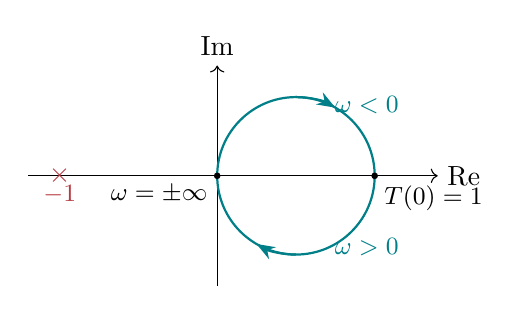
\begin{tikzpicture}[scale=2]
\draw[->] (-1.2,0)--(1.4,0) node[right]{$\Re$}; \draw[->] (0,-0.7)--(0,0.7) node[above]{$\Im$};
\draw[thick,teal] (0.5,0) circle (0.5);
\draw[-Stealth,thick,teal] (0.5,0.5) arc (90:60:0.5); \draw[-Stealth,thick,teal] (0.5,-0.5) arc (-90:-120:0.5);
\fill (1,0) circle (0.6pt) node[below right]{\small$T(0)=1$}; \fill (0,0) circle(0.6pt) node[below left]{\small$\omega=\pm\infty$};
\node[redx] at (-1,0) {$\times$}; \node[redx,below] at (-1,0) {\small$-1$};
\node[teal] at (0.95,0.45) {\small$\omega<0$}; \node[teal] at (0.95,-0.45) {\small$\omega>0$};
\end{tikzpicture}
\end{center}
It never winds round $-1$, so by Nyquist's criterion (Chapter 5) negative unit feedback keeps it stable; indeed $\frac{R}{1+R}=\frac{1}{s+2}$.
\end{workbox}

\begin{workbox}[title={Worked example \fr{145--146}: $ay''+by'+y=u$, $a,b>0$}]
$T(s)=\dfrac1{as^2+bs+1}$, so $T(i\omega)=\dfrac{1}{1-a\omega^2+ib\omega}=\dfrac{1-a\omega^2-ib\omega}{(1-a\omega^2)^2+b^2\omega^2}$.
\[\Gamma(\omega)=\frac1{\sqrt{(1-a\omega^2)^2+b^2\omega^2}},\qquad \tan\phi=\frac{b\omega}{a\omega^2-1},\quad\phi=\arg(1-a\omega^2-ib\omega).\]
$T(0)=1$ so $\phi(0)=0$; at $\omega=\pm1/\sqrt a$ the real part vanishes, $T(i\omega)$ is on the imaginary axis and $\phi=\mp\pi/2$;
as $\omega\to+\infty$, $T(i\omega)$ is in the third quadrant ($\phi\to-\pi$); as $\omega\to-\infty$, in the second quadrant.
\textbf{Special case} $T=\frac1{s^2+s+6}$ (the notes' Bode plot): $\Gamma=\frac1{\sqrt{(6-\omega^2)^2+\omega^2}}$, $\Gamma(0)=\frac16\approx-15.6$\,dB, phase passes $-90^\circ$ at $\omega=\sqrt6$ and tends to $-180^\circ$.
\end{workbox}

\begin{thmbox}[title={Proposition 0.40 (Nyquist's locus)}]
If $R$ is proper rational with all poles in the open LHP, then $\omega\mapsto R(i\omega)$ $(-\infty\le\omega\le\infty)$ is a closed contour of finite length starting and ending at $c=\lim_{s\to\infty}R(s)$.
\emph{Idea:} $R=c+\sum_jc_j(s-\lambda_j)^{-m_j}$, $\Re\lambda_j<-\delta$, so $|R'(i\omega)|\le M/(1+\omega^2)$, which is integrable.
\end{thmbox}

\subsection{Stability: the three cases for \texorpdfstring{$\dot X=AX$}{dX/dt=AX} \texorpdfstring{\fr{152}}{}}\label{sec:stab}\label{ss:4-3}
\begin{thmbox}[title={Stability of $\dot X=AX$, $X(t)=\exp(tA)X_0$}]
\renewcommand{\arraystretch}{1.3}
\begin{tabular}{@{}p{3.1cm}p{5.4cm}p{6.3cm}@{}}
\toprule
\textbf{Name} & \textbf{Definition} & \textbf{Eigenvalue test}\\\midrule
Exponentially stable & $\|X(t)\|\le Me^{-\delta t}$ for all $X_0$ & all $\Re\lambda_j<0$ $\quad(\Rightarrow$ BIBO stable$)$\\
Marginally stable & $X(t)$ bounded for all $X_0$ & all $\Re\lambda_j\le0$, and every $\lambda$ with $\Re\lambda=0$ has only $1\times1$ Jordan blocks (regarded as BIBO \emph{unstable})\\
Unstable & $X(t)$ unbounded for some $X_0$ & some $\Re\lambda_j>0$, or some $\Re\lambda=0$ with a Jordan block of size $\ge2$\\
\bottomrule
\end{tabular}
\end{thmbox}
\begin{methodbox}[title={Method: classify the stability of $\dot X=AX$}]
\begin{enumerate}
\item Find the eigenvalues (or just the signs of their real parts; see \S\ref{sec:stabpoly} for polynomial tests).
\item All $\Re\lambda<0$ $\Rightarrow$ exponentially stable. Any $\Re\lambda>0$ $\Rightarrow$ unstable. Stop.
\item If some $\Re\lambda=0$ (and none $>0$): check the Jordan blocks of those eigenvalues: geometric multiplicity $=$ algebraic $\Rightarrow$ marginal; otherwise unstable (a factor $t$ appears in $\exp(tA)$).
\end{enumerate}
\end{methodbox}
\begin{workbox}[title={Worked examples}]
\begin{itemize}
\item $A=\begin{bmatrix}-1&5\\0&-2\end{bmatrix}$: eigenvalues $-1,-2$ $\Rightarrow$ exponentially stable.
\item $A=\begin{bmatrix}0&1\\-1&0\end{bmatrix}$: $\pm i$, simple $\Rightarrow$ marginally stable ($\exp(tA)$ is a rotation, bounded).
\item $A=\begin{bmatrix}0&0\\0&0\end{bmatrix}$: $0$ twice, two $1\times1$ blocks $\Rightarrow$ marginally stable ($X(t)=X_0$).
\item $A=\begin{bmatrix}0&1\\0&0\end{bmatrix}=J_2(0)$: $\exp(tA)=\begin{bmatrix}1&t\\0&1\end{bmatrix}$ $\Rightarrow$ unstable ($X_0=[0;1]$ gives $X(t)=[t;1]$).
\item AE2's companion matrix for $s^4+2s^3+s^2+4s+2$: eigenvalues $0.35\pm1.28i$ $\Rightarrow$ unstable.
\end{itemize}
\end{workbox}

\begin{defbox}[title={BIBO stability \fr{153}}]
$(A,B,C,D)$ is \textbf{bounded-input bounded-output stable} if every bounded input $u$ on $(0,\infty)$ produces a bounded output $y$ on $(0,\infty)$.
\end{defbox}

\subsection{The damped harmonic oscillator \texorpdfstring{\fr{149--151}, \fr{169}}{}}\label{ss:4-4}
$y''+\beta y'+\gamma y=u$, $A=\begin{bmatrix}0&1\\-\gamma&-\beta\end{bmatrix}$, eigenvalues $\lambda_\pm=\frac12(-\beta\pm\sqrt\Delta)$ with $\Delta=\beta^2-4\gamma$, eigenvectors $[1;\lambda_\pm]$.
For $\lambda_+\neq\lambda_-$, $S=\begin{bmatrix}1&1\\\lambda_+&\lambda_-\end{bmatrix}$ and $\exp(tA)=S\,\mathrm{diag}(e^{t\lambda_+},e^{t\lambda_-})S^{-1}$.
\begin{center}
\renewcommand{\arraystretch}{1.3}
\begin{tabular}{@{}lccc@{}}
\toprule
($\gamma>0$) & $\Delta<0$ & $\Delta=0$ & $\Delta>0$\\\midrule
$\beta>0$ (stable) & decaying oscillations & critically damped & exponential decay\\
$\beta=0$ (marginal) & periodic & --- & ---\\
$\beta<0$ (unstable) & unbounded oscillations & exponential growth & exponential growth\\
\bottomrule
\end{tabular}
\end{center}
\textbf{The damped oscillator is exponentially stable iff $\beta>0$ and $\gamma>0$} (both coefficients of $s^2+\beta s+\gamma$ positive). $\beta=0,\gamma>0$: marginal.

\subsection{Resonance: marginal is not BIBO \texorpdfstring{\fr{154--157}}{}}\label{ss:4-5}
\begin{workbox}[title={Undamped oscillator $\ddot x+\nu^2x=U_0\cos\omega t$}]
$A=\begin{bmatrix}0&1\\-\nu^2&0\end{bmatrix}$, eigenvalues $\pm i\nu$ (simple) $\Rightarrow$ marginally stable.
Complementary function $c_1\begin{bmatrix}\cos\nu t\\-\nu\sin\nu t\end{bmatrix}+c_2\begin{bmatrix}\sin\nu t\\\nu\cos\nu t\end{bmatrix}$ (bounded).
\begin{itemize}
\item $\omega\neq\nu$: particular integral $\dfrac{U_0}{\nu^2-\omega^2}\begin{bmatrix}\cos\omega t\\-\omega\sin\omega t\end{bmatrix}$, bounded.
\item $\omega=\nu$ (\textbf{resonance}): particular integral $\dfrac{U_0}{2\nu}\begin{bmatrix}t\sin\nu t\\\sin\nu t+\nu t\cos\nu t\end{bmatrix}$, \textbf{unbounded}.
\end{itemize}
Bounded input, unbounded output $\Rightarrow$ \textbf{not BIBO stable}. Laplace view: $T(s)=\frac1{s^2+\nu^2}$ and $\hat u=\frac{U_0s}{s^2+\nu^2}$, so $\hat x$ has a \emph{double} pole at $\pm i\nu$, giving $t\sin\nu t$.
\end{workbox}

\subsection{BIBO stability theorems \texorpdfstring{\fr{158--161}, \fr{170--172}}{}}\label{ss:4-6}
\begin{thmbox}[title={Theorem 0.42 (frame 159)}]
If every eigenvalue of $A$ has $\Re\lambda_j<0$ and $U$ is bounded on $(0,\infty)$, then all solutions of $(A,B,C,D)$ are bounded; so $(A,B,C,D)$ is BIBO stable.
\end{thmbox}
\begin{proofbox}[title={Proof of Theorem 0.42 (learn this one)}]
By Lemma 0.41 there are $M,\delta>0$ with $\|\exp(tA)\|\le Me^{-\delta t}$, and by hypothesis $\|B\|\|U(v)\|\le K$. From Theorem 0.17,
\begin{align*}
\|X(t)\|&\le\|\exp(tA)\|\|X_0\|+\int_0^t\|\exp((t-v)A)\|\,\|B\|\,\|U(v)\|\,dv
\le M\|X_0\|+KM\int_0^te^{-\delta(t-v)}dv\\
&=M\|X_0\|+\frac{KM}{\delta}\big(1-e^{-\delta t}\big)\le M\|X_0\|+\frac{KM}{\delta}.
\end{align*}
So $X$ is bounded, and $Y=CX+DU$ is a sum of bounded functions, hence bounded.
\end{proofbox}

\begin{thmbox}[title={Theorem 0.45 (frame 170): stable $T$ $\iff$ BIBO stable realisation}]
A complex rational $T$ is \textbf{stable} (proper, all poles in the open LHP) iff $T$ is the transfer function of some BIBO stable $(A,B,C,D)$.
\end{thmbox}
\begin{proofbox}[title={Proof outline of Theorem 0.45}]
($\Rightarrow$ BIBO gives stable $T$.) Take the bounded input $u=1$, $\hat u=\frac1s$. If $|y|\le M$ then $|\hat Y(s)|\le\int_0^\infty e^{-t\Re s}M\,dt=\frac{M}{\Re s}$, so $\hat Y$ is holomorphic on $\Re s>0$ and $\to0$ as $s\to\infty$ along $(0,\infty)$; hence $T=s\hat Y$ is proper.
A pole $\lambda$ with $\Re\lambda>0$ would also be a pole of $\hat Y=T/s$, impossible since $\hat Y$ is holomorphic there.
A pole $\lambda=i\nu$ on the axis: use the bounded input $\cos\nu t$, $\hat u=\frac{s}{s^2+\nu^2}$, which has a pole at $i\nu$, so $T\hat u$ blows up like $(s-i\nu)^{-2}$ or worse; but $|\hat Y(s)|\le M/\Re s$ only allows $(s-i\nu)^{-1}$ type growth. Contradiction (resonance). So all poles are in the LHP.\\
($\Leftarrow$) If $T$ is stable, the companion realisation (Prop 0.22) has eigenvalues of $A$ = poles of $T$, all with $\Re<0$, so it is BIBO stable by Theorem 0.42.
\end{proofbox}
\begin{exambox}
\begin{itemize}
\item ``Is the system BIBO stable?'': compute the eigenvalues of $A$; if all $\Re<0$, cite Theorem 0.42.
\item ``Is $T$ stable?'': check it is \textbf{proper} and all poles have $\Re<0$. Forgetting properness loses marks: $T=s^2/(s+1)$ has its pole in the LHP but is \emph{not} stable.
\item $T=\frac1s$ (an integrator) is not BIBO stable: the bounded input $u=1$ gives $y=t$.
\end{itemize}
\end{exambox}

\subsection{Exam-style questions for Chapter 4}\label{ss:4-7}
\begin{qbox}[title={Q4.1 (classification)}]
For each $A$, decide whether $\dot X=AX$ is exponentially stable, marginally stable or unstable:
(a) $\begin{bmatrix}-2&1\\-1&-2\end{bmatrix}$, (b) $\begin{bmatrix}0&2\\-2&0\end{bmatrix}$, (c) $\begin{bmatrix}1&0\\0&-3\end{bmatrix}$, (d) $\begin{bmatrix}0&1&0\\0&0&0\\0&0&-1\end{bmatrix}$.
\end{qbox}
\begin{solbox}
(a) $\chi=(s+2)^2+1$, $\lambda=-2\pm i$: exponentially stable. (b) $\chi=s^2+4$, $\lambda=\pm2i$ simple: marginal. (c) $\lambda=1>0$: unstable.
(d) $\lambda=0$ (algebraic multiplicity 2) and $\lambda=-1$. $A-0I=A$ has rank 2 (rows $(0,1,0)$ and $(0,0,-1)$), so $\dim E(0)=3-2=1<2$: there is a $J_2(0)$ block, so \textbf{unstable} ($X_0=e_2$ gives $X(t)=[t;1;0]$).
\end{solbox}

\begin{qbox}[title={Q4.2 (gain and phase)}]
$T(s)=\dfrac{2}{s+2}$. Find $\Gamma(\omega)$ and $\phi(\omega)$, the gain in dB at $\omega=2$, and the steady-state output for input $\cos2t$.
\end{qbox}
\begin{solbox}
$T(i\omega)=\frac{2}{2+i\omega}$: $\Gamma=\frac{2}{\sqrt{4+\omega^2}}$, $\phi=-\tan^{-1}(\omega/2)$ (real part $>0$). At $\omega=2$: $\Gamma=\frac1{\sqrt2}$, $20\log_{10}\frac1{\sqrt2}\approx-3.01$ dB, $\phi=-\frac\pi4$ (phase lag).
Steady state: $\cos2t=\Re e^{2it}\mapsto\Re\big(T(2i)e^{2it}\big)=\frac1{\sqrt2}\cos(2t-\frac\pi4)$.
\end{solbox}

\begin{qbox}[title={Q4.3 (BIBO and resonance)}]
Is the system $\ddot y+9y=u$ BIBO stable? Justify by choosing an input.
\end{qbox}
\begin{solbox}
$T(s)=\frac1{s^2+9}$, poles $\pm3i$ on the imaginary axis, so $T\notin\mathcal S$, not BIBO stable (Theorem 0.45). Explicitly, $u=\cos3t$ (bounded) gives
$\hat y=\frac{s}{(s^2+9)^2}=-\frac12\frac{d}{ds}\frac{1}{s^2+9}$, so $y=\frac{t}{2}\cdot\frac{\sin3t}{3}=\frac{t\sin3t}{6}$, unbounded. (Zero initial data.)
\end{solbox}
\newpage

\section{Chapter 5: Feedback control \texorpdfstring{\fr{162--218}}{}}
\label{ch5}

\subsection*{Big picture}
Chapter 4 told us how to \emph{recognise} stability. Chapter 5 is about \emph{creating} it by feedback, using only algebra on transfer functions:
\begin{enumerate}
\item test polynomials for stability without finding roots (Maxwell's problem);
\item the ring $\mathcal S$ of stable rational functions;
\item Nyquist's criterion (stability under feedback from a picture);
\item the simple feedback loop $T=\frac{G}{1+GK}$, PID controllers;
\item a guaranteed recipe to stabilise \emph{any} rational plant: coprime factorisation $\to$ Youla controller $K=X/Y$;
\item matrix tools: positive definite matrices, Lyapunov's criterion, Sylvester's equation.
\end{enumerate}

\subsection{Stable polynomials \texorpdfstring{\fr{163--164}}{}}\label{sec:stabpoly}\label{ss:5-1}
\begin{plainbox}
A polynomial is \textbf{stable} if all its roots are in the left half plane (so the matching terms $e^{\lambda t}$ decay).
Quick test without finding roots: a stable polynomial must have \textbf{all coefficients positive}. That is enough for degree 2,
but not for degree 3 or more (use $a_2a_1>a_0$ for degree 3).
\par\smallskip\textbf{In the exam this looks like:} ``Is this polynomial stable?'', ``for which $k$ is it stable?'', ``prove all coefficients are positive''.
\end{plainbox}
\begin{defbox}
A polynomial $h$ is \textbf{stable} if all its zeros lie in the open left half plane LHP $=\{s:\Re s<0\}$.
(So $h$ stable $\iff$ $1/h$ is a stable rational function.)
\end{defbox}
\begin{thmbox}[title={Proposition 0.43 (necessary condition)}]
If $h$ is a \textbf{monic real} stable polynomial then \textbf{all its coefficients are positive}.
\end{thmbox}
\begin{proofbox}[title={Proof of Proposition 0.43}]
Real coefficients $\Rightarrow$ $h(\lambda)=0\iff h(\bar\lambda)=0$. So the roots are real $\mu_j<0$, or conjugate pairs $\lambda_k,\bar\lambda_k$ with $\Re\lambda_k<0$, giving
$(s-\lambda_k)(s-\bar\lambda_k)=s^2-2\Re\lambda_k\,s+|\lambda_k|^2$. Hence
$h(s)=\prod_j(s-\mu_j)\prod_k(s^2-2\Re\lambda_k\,s+|\lambda_k|^2)$ with $-\mu_j>0$, $-2\Re\lambda_k>0$, $|\lambda_k|^2>0$.
Multiplying out polynomials with positive coefficients gives positive coefficients.
\end{proofbox}
\begin{warnbox}
The converse is \textbf{false} for degree $\ge3$: $s^3+s^2+s+1=(s+1)(s^2+1)$ has positive coefficients but roots $\pm i$. The AE2 polynomial $s^4+2s^3+s^2+4s+2$ also has positive coefficients but is unstable.
So use positivity only to \emph{rule out} stability (a zero or negative coefficient $\Rightarrow$ not stable).
\end{warnbox}
\begin{thmbox}[title={Useful tests by degree (degree 3 is Routh's extension, \emph{not proved} in the notes)}]
\begin{itemize}
\item Degree 1: $s+a_0$ stable $\iff a_0>0$.
\item Degree 2: $s^2+a_1s+a_0$ stable $\iff a_1>0$ and $a_0>0$. (Proof: roots $\frac{-a_1\pm\sqrt{a_1^2-4a_0}}2$; this is the damped oscillator table.)
\item Degree 3: $s^3+a_2s^2+a_1s+a_0$ stable $\iff a_2,a_1,a_0>0$ and $\boxed{a_2a_1>a_0}$.
\item Any degree: form the companion matrix and compute its eigenvalues numerically \fr{163}.
\end{itemize}
If you use the degree-3 test, say ``by the Routh--Hurwitz criterion''; when $a_2a_1=a_0$ the polynomial factorises as $(s+a_2)(s^2+a_1)$ with roots on the imaginary axis.
\end{thmbox}

\subsection{The ring \texorpdfstring{$\mathcal S$}{S} of stable rational functions \texorpdfstring{\fr{165--169}}{}}\label{ss:5-2}
\begin{plainbox}
$\mathcal S$ is the set of ``safe'' transfer functions: \textbf{proper} (does not blow up at high frequency) and all poles on the
left (does not blow up in time). Adding or multiplying safe functions gives safe functions.
\par\smallskip\textbf{In the exam this looks like:} ``Is $f\in\mathcal S$?'' or ``show $\mathcal S$ is not a field''.
\end{plainbox}
\begin{defbox}
$f=g/h$ is a \textbf{stable rational function}, $f\in\mathcal S$, if (i) $f$ is \textbf{proper} ($\deg g\le\deg h$) and (ii) all poles lie in the open LHP ($h$ stable).
\end{defbox}
\begin{thmbox}[title={Proposition 0.44}]
$\mathcal S$ is a commutative differential ring (closed under $+$, $\times$, scalar multiples and $d/ds$, Leibniz rule; no zero divisors on RHP). But $\mathcal S$ is \textbf{not a field}:
$\frac1{s+1}\in\mathcal S$ but its inverse $s+1$ is not proper, so $s+1\notin\mathcal S$.
\end{thmbox}
\begin{proofbox}[title={Proof sketch (closure)}]
Product: $\frac{g_1g_2}{h_1h_2}$ has $\deg(g_1g_2)\le\deg(h_1h_2)$ and the zeros of $h_1h_2$ are zeros of $h_1$ or $h_2$, so in the LHP.
Sum: $\frac{g_1h_2+g_2h_1}{h_1h_2}$, same reasoning. Derivative: by partial fractions $f=q+\sum a_j(s-\lambda_j)^{-n_j}$ with $q$ constant and $\Re\lambda_j<0$, so
$f'=\sum -n_ja_j(s-\lambda_j)^{-n_j-1}$ is strictly proper with the same poles.
\end{proofbox}

\subsection{Nyquist's criterion \texorpdfstring{\fr{174--177}}{}}\label{ss:5-3}
\begin{plainbox}
Look at the picture of $R(i\omega)$. If it never loops around the point $-1$, then closing the loop (feeding the output back
negatively) keeps the system stable. Where the curve crosses the negative real axis tells you how much extra gain you can add
before it becomes unstable.
\par\smallskip\textbf{In the exam this looks like:} ``Use Nyquist's criterion to find the values of $k$ for which the closed loop is stable''.
\end{plainbox}
\begin{thmbox}[title={Nyquist's criterion}]
Let the plant $R$ be \textbf{stable}. If the Nyquist contour $R(i\omega)$, $-\infty\le\omega\le\infty$, does \textbf{not pass through or wind around $-1$}, then
$T=\dfrac{R}{1+R}$ is stable, i.e.\ the feedback loop with constant feedback $-1$ is stable.\\
\textbf{Argument principle:} $N=Z-P$ where $N$ = net number of \textbf{clockwise} windings of $R(i\omega)$ round $-1$, $Z$ = number of zeros of $1+R$ in the RHP, $P$ = number of poles of $1+R$ in the RHP.
Here $P=0$ ($R$ stable) and $N=0$, so $Z=0$: no closed-loop poles in the RHP.
\end{thmbox}
\begin{proofbox}[title={Why $T$ is proper and where its poles can be \fr{175}}]
Write $R=c+p/q$ with $\deg p<\deg q$, $c=\lim_{s\to\infty}R\neq-1$. Then $T=\dfrac{cq+p}{(1+c)q+p}$, and $\deg((1+c)q+p)=\deg q$, so $T$ is proper.
A pole of $R$ gives a finite value of $T=R/(1+R)$, so the only possible poles of $T$ are zeros of $1+R$; the argument principle locates them.
\end{proofbox}
\begin{methodbox}[title={Method: use Nyquist to find a gain margin}]
\begin{enumerate}
\item Find where $R(i\omega)$ crosses the negative real axis: solve $\Im R(i\omega)=0$ (equivalently $\phi(\omega)=-\pi$).
\item Compute $R(i\omega)$ there. If it lies to the right of $-1$, no winding $\Rightarrow$ stable feedback loop.
\item With a gain $k$, the crossing point scales by $k$: stable while $k\,|R(i\omega_c)|<1$.
\end{enumerate}
\end{methodbox}
\begin{workbox}[title={Worked example: $R(s)=\dfrac{k}{(s+1)^3}$, $k>0$}]
\textbf{Nyquist.} $\phi(\omega)=-3\tan^{-1}\omega=-\pi$ at $\omega=\sqrt3$, where $|R|=\frac{k}{(1+3)^{3/2}}=\frac k8$. The plot crosses the negative real axis at $-k/8$, so it avoids winding round $-1$ iff $k<8$.\\
\textbf{Check algebraically.} Closed-loop denominator $(s+1)^3+k=s^3+3s^2+3s+(1+k)$: Routh needs $3\cdot3>1+k$, i.e.\ $k<8$ \checkmark. At $k=8$: $(s+3)(s^2+3)$, roots $\pm i\sqrt3$ (exactly the crossing frequency).
\end{workbox}

\subsection{The simple feedback loop and PID control \texorpdfstring{\fr{179--185}}{}}\label{sec:pid}\label{ss:5-4}
\begin{plainbox}
A \textbf{controller} watches the output and corrects the input, like cruise control. With negative feedback through $K$, the new
transfer function is $T=G/(1+GK)$. We choose $K$ (often $a+b/s+cs$, a PID) so that the new denominator is a stable polynomial.
\par\smallskip\textbf{In the exam this looks like:} ``Find a controller of the form $-a-b/s$ that stabilises $G$'' --- set up the denominator and choose $a,b$.
\end{plainbox}
\begin{center}
\begin{tikzpicture}
\node (u) at (0,0) {$u$}; \node[sumj] (s) at (1.3,0) {$+$}; \node[blk] (g) at (3,0) {$G$}; \node[tap] (t) at (4.4,0) {}; \node (y) at (5.4,0) {$y$};
\node[blk] (k) at (3,1.2) {$-K$};
\draw[ar] (u)--(s); \draw[ar] (s)--(g); \draw[ar] (g)--(t); \draw[ar] (t)--(y); \draw[ar] (t)|-(k); \draw[ar] (k)-|node[left,pos=.8]{$-Ky$}(s);
\end{tikzpicture}
\end{center}
\begin{thmbox}[title={Simple feedback loop (SFL)}]
Plant $G$ ($m\times k$), controller $-K$ ($k\times m$, negative feedback). From $y=G(u-Ky)$:
\[\boxed{T=(I+GK)^{-1}G}\qquad\text{(SISO: }T=\frac{G}{1+GK}\text{).}\]
Poles of $G$: \textbf{open-loop poles}; poles of $T$: \textbf{closed-loop poles}. If $G=p/q$ and $K=k$ (constant), $T=\dfrac{p}{kp+q}$.
\textbf{PID controller:} $K(s)=a+\dfrac bs+cs$ (proportional + integral + derivative). PD: abrupt correction (Whitehead's torpedoes); PI: gentle.
\end{thmbox}
\begin{methodbox}[title={Method: choose a controller to stabilise $G$}]
\begin{enumerate}
\item Write $T=\dfrac{G}{1+GK}=\dfrac{1}{1/G+K}$ and clear fractions to get $T=\dfrac{\text{num}}{\text{closed-loop polynomial}}$.
\item Write the closed-loop polynomial with the controller parameters as unknowns.
\item Impose the stability test (positive coefficients for degree 2; Routh for degree 3).
\item Choose nice values (e.g.\ make the polynomial $(s+1)^2$), and check that $T$ is \textbf{proper}.
\end{enumerate}
\end{methodbox}
\begin{workbox}[title={Worked example \fr{185}: stabilise $G(s)=\dfrac{s}{(s-1)(s+3)}$ by a PI controller}]
Open-loop poles $1,-3$: unstable. Take $K(s)=-a-\frac bs$ in $T=\frac{G}{1+GK}$ (this is the notes' sign convention). Then
\[\frac{1}{G}+K=\frac{(s-1)(s+3)}{s}-a-\frac bs=\frac{s^2+2s-3-as-b}{s},\qquad T=\frac{s}{s^2+(2-a)s-(b+3)}.\]
Need $2-a>0$ and $-(b+3)>0$. Choose $a=0$, $b=-4$: $T=\dfrac{s}{s^2+2s+1}=\dfrac{s}{(s+1)^2}\in\mathcal S$. So $K(s)=\frac4s$ (pure integral feedback) works.
\end{workbox}
\begin{warnbox}
Sign conventions differ: the diagram has the block $-K$ and the formula uses $K$. State your convention once, e.g.\ ``with $T=G/(1+GK)$'', and stick to it.
\end{warnbox}
\begin{workbox}[title={Worked example \fr{184}: proportional feedback can fix an improper plant}]
$G=\frac{s^2}{bs+c}$ ($b,c>0$) is not proper. With $K=k>0$: $T=\dfrac{s^2}{ks^2+bs+c}$, proper, poles $\frac{-b\pm\sqrt{b^2-4ck}}{2k}$ in the LHP (positive coefficients, degree 2). Stable.
\end{workbox}

\subsection{Euclid, B\'ezout and matrix completion \texorpdfstring{\fr{186--193}}{}}\label{ss:5-5}
\begin{plainbox}
The Euclidean algorithm finds the \textbf{highest common factor} of two polynomials by repeated long division, exactly like for
whole numbers. Working backwards writes $1=PM+QN$ whenever $P,Q$ have no common root. This identity is the engine of the next subchapter.
\par\smallskip\textbf{In the exam this looks like:} ``Find polynomials $M,N$ with $PM+QN=1$'' or ``complete this matrix to an invertible one''.
\end{plainbox}
\begin{methodbox}[title={Euclidean algorithm and B\'ezout for polynomials}]
\begin{enumerate}
\item Divide: $P_0=Q_1P_1+P_2$ with $\deg P_2<\deg P_1$; then $P_1=Q_2P_2+P_3$, and so on until a remainder is $0$. The last nonzero remainder $P_n$ is the highest common factor.
\item \textbf{Work back}: $P_n=P_{n-2}-Q_{n-1}P_{n-1}$, substitute for $P_{n-1}$, etc., to get $P_n=MP_0+NP_1$.
\item If $P_n$ is a nonzero constant $r$, divide by $r$ to get $MP_0/r+NP_1/r=1$.
\end{enumerate}
MATLAB: \texttt{[g,M,N]=gcd(P,Q)}. All in exact arithmetic, no roots needed.
\end{methodbox}
\begin{thmbox}[title={Lemma 0.47 and Proposition 0.48}]
Nonzero $P,Q\in\CC[s]$ have \textbf{no common zeros} $\iff$ $\exists$ polynomials $M,N$ with $PM+QN=1$.\\
For $f,g\in\CC[s]$ TFAE: (1) $\begin{bmatrix}f&g\\h&k\end{bmatrix}$ can be completed to a matrix with polynomial inverse; (2) $fk-gh=\Delta\in\CC\setminus\{0\}$; (3) hcf$(f,g)=1$; (4) $f,g$ have no common zeros.
\end{thmbox}
\begin{proofbox}[title={Proof of Lemma 0.47}]
($\Leftarrow$) If $\lambda$ were a common zero, $1=P(\lambda)M(\lambda)+Q(\lambda)N(\lambda)=0$, contradiction.
($\Rightarrow$) Euclid gives $PM+QN=R$ with $R$ the hcf. If $R=r$ is a nonzero constant, divide by $r$. Otherwise $\deg R\ge1$, so $R$ has a zero $\lambda$ (fundamental theorem of algebra); $R$ divides $P$ and $Q$, so $\lambda$ is a common zero, contradiction.
\end{proofbox}
\begin{workbox}[title={Worked examples}]
\textbf{(a) hcf.} $P_0=s^3+2s^2+s+2$, $P_1=s^2+3s+2$: $P_0=(s-1)P_1+(2s+4)$; $P_1=(\frac s2+\frac12)(2s+4)+0$. hcf $=2s+4\sim s+2$, and $2s+4=P_0-(s-1)P_1$.\\
\textbf{(b) B\'ezout.} $P=s+2$, $Q=s^2+1$: $Q=(s-2)P+5$, so $5=Q-(s-2)P$ and $\boxed{1=\tfrac15Q-\tfrac{s-2}5P}$. (Check: $\frac{s^2+1-(s^2-4)}5=1$ \checkmark)\\
\textbf{(c) Completion.} With $f=s+2$, $g=s^2+1$ take $k=\frac{2-s}5$, $h=-\frac15$: $fk-gh=\frac{4-s^2+s^2+1}5=1$, so $F=\begin{bmatrix}s+2&s^2+1\\-\frac15&\frac{2-s}5\end{bmatrix}$ has inverse $\begin{bmatrix}\frac{2-s}5&-(s^2+1)\\\frac15&s+2\end{bmatrix}$.\\
\textbf{(d) Integers} \fr{191}: $\begin{bmatrix}3&5\\c&d\end{bmatrix}$ has an integer inverse iff $3d-5c=\pm1$, e.g.\ $c=1,d=2$; possible because $\gcd(3,5)=1$.
\end{workbox}

\subsection{Coprime factorisation in \texorpdfstring{$\mathcal S$}{S} \texorpdfstring{\fr{194--200}}{}}\label{sec:coprime}\label{ss:5-6}
\begin{plainbox}
Goal: a \textbf{recipe that stabilises any plant}. Write $G=P/Q$ using only ``safe'' functions (the substitution $\lambda=1/(1+s)$ does this),
find $X,Y$ with $PX+QY=1$ (Euclid), and take the controller $K=X/Y$. Then all closed-loop functions are products of safe functions, so safe.
\par\smallskip\textbf{In the exam this looks like:} ``Find a coprime factorisation and a stabilising controller, and verify''. A long question, but purely mechanical.
\end{plainbox}
\begin{defbox}
$P,Q\in\mathcal S$ are \textbf{coprime} if there are $X,Y\in\mathcal S$ with $PX+QY=1$.
\textbf{Proposition 0.49:} every rational $G$ can be written $G=P/Q$ with $P,Q$ coprime in $\mathcal S$, found in exact arithmetic.
\end{defbox}
\begin{methodbox}[title={The coprime factorisation algorithm (4 steps)}]
\begin{enumerate}
\item Write $G=M(s)/N(s)$ with polynomials $M,N$ having \textbf{no common zeros}; let $m=\max(\deg M,\deg N)$.
\item Substitute $s=\dfrac{1-\lambda}{\lambda}$ (i.e.\ $\lambda=\dfrac1{1+s}$) and clear denominators: $\tilde M(\lambda)=\lambda^mM\big(\frac{1-\lambda}\lambda\big)$, $\tilde N(\lambda)=\lambda^mN\big(\frac{1-\lambda}\lambda\big)$.
\item Euclid/B\'ezout in $\lambda$: find polynomials $\tilde X,\tilde Y$ with $\tilde M\tilde X+\tilde N\tilde Y=1$.
\item Put back $\lambda=\dfrac1{1+s}$: $P=\tilde M,\ Q=\tilde N,\ X=\tilde X,\ Y=\tilde Y$ evaluated at $\frac1{1+s}$. All four are polynomials in $\frac1{1+s}$, so proper with only pole $-1$: they lie in $\mathcal S$.
\end{enumerate}
\end{methodbox}
\begin{thmbox}[title={Proposition 0.50 and Theorem 0.52 (Youla)}]
If $G=P/Q$ with $PX+QY=1$ in $\mathcal S$, then the controller $\boxed{K=X/Y}$ gives
\[\frac{1}{1+GK}=QY,\quad\frac{G}{1+GK}=PY,\quad\frac{K}{1+GK}=XQ,\quad\frac{GK}{1+GK}=PX,\]
all in $\mathcal S$. So $K=X/Y$ \textbf{internally stabilises} the SFL. Every rational SISO can be stabilised by a rational (possibly unstable) controller.
\end{thmbox}
\begin{proofbox}[title={Proof (one line each)}]
$1+GK=1+\frac{PX}{QY}=\frac{QY+PX}{QY}=\frac1{QY}$. Hence $\frac1{1+GK}=QY$, $\frac{G}{1+GK}=\frac PQ\,QY=PY$, $\frac{K}{1+GK}=\frac XY\,QY=XQ$, $\frac{GK}{1+GK}=\frac{PX}{QY}QY=PX$.
Products of elements of $\mathcal S$ are in $\mathcal S$.
\end{proofbox}

\begin{workbox}[title={Worked example A: $G(s)=\dfrac1{s-1}$}]
\textbf{1.} $M=1$, $N=s-1$, $m=1$.\quad
\textbf{2.} $\tilde M=\lambda$, $\tilde N=\lambda\big(\frac{1-\lambda}\lambda-1\big)=1-2\lambda$.\quad
\textbf{3.} By inspection $2\tilde M+1\cdot\tilde N=1$: $\tilde X=2$, $\tilde Y=1$.\\
\textbf{4.} $P=\frac1{1+s}$, $Q=1-\frac2{1+s}=\frac{s-1}{s+1}$, $X=2$, $Y=1$. Check $P/Q=\frac1{s-1}$ \checkmark. Controller $K=X/Y=2$:
$\frac{G}{1+GK}=\frac1{s+1}$, $\frac1{1+GK}=\frac{s-1}{s+1}$, $\frac{K}{1+GK}=\frac{2(s-1)}{s+1}$, $\frac{GK}{1+GK}=\frac2{s+1}$, all in $\mathcal S$.
\end{workbox}

\begin{workbox}[title={Worked example B: $G(s)=\dfrac1{s^2}$ (double integrator)}]
\textbf{1.} $M=1$, $N=s^2$, $m=2$.\quad
\textbf{2.} $\tilde M=\lambda^2$, $\tilde N=(1-\lambda)^2=\lambda^2-2\lambda+1$.\\
\textbf{3.} Euclid: $\tilde N=1\cdot\tilde M+(1-2\lambda)$; \ $\tilde M=\lambda^2=(1-2\lambda)\big(-\frac\lambda2-\frac14\big)+\frac14$. Work back:
$\frac14=\tilde M+(1-2\lambda)\big(\frac\lambda2+\frac14\big)=\tilde M+(\tilde N-\tilde M)\big(\frac\lambda2+\frac14\big)=\tilde M\big(\tfrac34-\tfrac\lambda2\big)+\tilde N\big(\tfrac\lambda2+\tfrac14\big)$.
Times 4: $\tilde M(3-2\lambda)+\tilde N(1+2\lambda)=1$.\\
\textbf{4.} $P=\frac1{(1+s)^2}$, $Q=\frac{s^2}{(1+s)^2}$, $X=3-\frac2{1+s}=\frac{3s+1}{s+1}$, $Y=1+\frac2{1+s}=\frac{s+3}{s+1}$; controller $K=\dfrac{3s+1}{s+3}$.\\
\textbf{Check:} $1+GK=\frac{s^2(s+3)+3s+1}{s^2(s+3)}=\frac{(s+1)^3}{s^2(s+3)}$, so $\frac{G}{1+GK}=\frac{s+3}{(s+1)^3}$, $\frac1{1+GK}=\frac{s^2(s+3)}{(s+1)^3}$, $\frac{K}{1+GK}=\frac{s^2(3s+1)}{(s+1)^3}$, $\frac{GK}{1+GK}=\frac{3s+1}{(s+1)^3}$: all proper with poles only at $-1$ \checkmark
\end{workbox}

\begin{workbox}[title={Worked example C \fr{196}: $G(s)=\dfrac{s^2+5}{s^2-s+1}$}]
With $s=\frac{1-\lambda}{\lambda}$, $m=2$: $\tilde M=6\lambda^2-2\lambda+1$, $\tilde N=3\lambda^2-3\lambda+1$, and Euclid gives
$\big(\tfrac{24\lambda-2}{7}\big)\tilde N-\big(\tfrac{12\lambda-9}{7}\big)\tilde M=1$. So $\tilde Y=\frac{24\lambda-2}7$, $\tilde X=-\frac{12\lambda-9}{7}$, and with $\lambda=\frac1{1+s}$:
$Y=\frac{22-2s}{7(1+s)}$, $X=\frac{9s-3}{7(1+s)}$, giving the stabilising controller $K=\dfrac XY=\dfrac{9s-3}{22-2s}$ (itself unstable, pole at $s=11$, which is allowed).
Indeed $\frac{G}{1+GK}=\frac{-2(s-11)(s^2+5)}{7(s+1)^3}\in\mathcal S$.
\end{workbox}

\subsection{Well-posedness and internal stability \texorpdfstring{\fr{201--206}}{}}\label{sec:internal}\label{ss:5-7}
\begin{plainbox}
It is not enough for the output to behave: \textbf{every signal inside the loop} must stay bounded too. If the controller cancels an
unstable part of the plant, the problem is hidden, not removed. So we check all four functions, not just $G/(1+GK)$.
\par\smallskip\textbf{In the exam this looks like:} ``Is the loop internally stable?'', ``when is the SFL well posed?''.
\end{plainbox}
\begin{thmbox}[title={Lemma 0.51}]
SFL with inputs $r,d,n$ and states $x=r-z$, $y=d+Kx$, $z=n+Gy$, i.e.\ $\begin{bmatrix}1&0&1\\-K&1&0\\0&-G&1\end{bmatrix}\begin{bmatrix}x\\y\\z\end{bmatrix}=\begin{bmatrix}r\\d\\n\end{bmatrix}$.
It is \textbf{well posed} (inputs determine states uniquely) iff $1+GK\neq0$, and then
\[\begin{bmatrix}x\\y\\z\end{bmatrix}=\frac1{1+GK}\begin{bmatrix}1&-G&-1\\K&1&-K\\GK&G&1\end{bmatrix}\begin{bmatrix}r\\d\\n\end{bmatrix}=\Phi\begin{bmatrix}r\\d\\n\end{bmatrix}.\]
\textbf{Internally stable}: every entry of $\Phi$ is in $\mathcal S$, i.e.\ $\frac1{1+GK},\frac G{1+GK},\frac{GK}{1+GK},\frac K{1+GK}\in\mathcal S$.
\end{thmbox}
\begin{exambox}[title={Why we need all four (a classic exam trap)}]
$G=\frac{s-1}{s+1}$, $K=\frac{1}{s-1}$ (the controller cancels the plant's RHP zero). Then $GK=\frac1{s+1}$ and
$\frac1{1+GK}=\frac{s+1}{s+2}$, $\frac{G}{1+GK}=\frac{s-1}{s+2}$, $\frac{GK}{1+GK}=\frac{1}{s+2}$ are all stable, \textbf{but}
$\frac{K}{1+GK}=\frac{s+1}{(s-1)(s+2)}$ has a pole at $1$. So the loop is \textbf{not internally stable}: an unstable pole--zero cancellation hides inside the loop, and the internal signal $y$ responds to the reference $r$ through the unstable $\frac{K}{1+GK}$, so it blows up even though the output $z$ looks fine.
\end{exambox}

\subsection{Self-adjoint and positive definite matrices \texorpdfstring{\fr{207--209}}{}}\label{sec:posdef}\label{ss:5-8}
\begin{plainbox}
A \textbf{positive definite} matrix is the matrix version of a positive number: $\langle Kz,z\rangle>0$ for every nonzero $z$.
Three equivalent tests: the definition, all eigenvalues positive, or all top-left determinants positive (easiest by hand).
\par\smallskip\textbf{In the exam this looks like:} ``Show that $S'KS$ / $\exp(A')K\exp(A)$ / $K+L$ is positive definite'' (AE3, A3.4).
\end{plainbox}
\begin{thmbox}
\begin{itemize}
\item \textbf{Prop 0.53:} if $A=A'$ then the eigenvalues are real and $A=U\Delta U'$ with $U$ unitary ($U'U=I$) and $\Delta$ real diagonal; eigenvectors for distinct eigenvalues are orthogonal.
\item $K$ is \textbf{positive definite} if $K=K'$ and $\langle Kz,z\rangle>0$ for all $z\neq0$.
\item \textbf{Lemma 0.54:} for $K=K'$, TFAE: (1) $\langle Kz,z\rangle>0\ \forall z\neq0$; (2) all eigenvalues $\kappa_j>0$; (3) all \textbf{leading principal minors} $\Delta_j>0$.
\item The product of positive definite matrices is generally \textbf{not} positive definite.
\end{itemize}
\end{thmbox}
\begin{workbox}[title={Worked example (AE3, A3.4): all five parts}]
$K$ real symmetric positive definite.\\
\textbf{(i)} If $Kv=\kappa v$, $v\neq0$: $0<\langle Kv,v\rangle=\langle\kappa v,v\rangle=\kappa\|v\|^2$, so $\kappa>0$ (in particular real).\\
\textbf{(ii)} $K$ is diagonalisable (Prop 0.53), so $\det K=\prod\kappa_j>0$ and $\tr K=\sum\kappa_j>0$.\\
\textbf{(iii)} $(S'KS)'=S'K'S''=S'KS$, so self-adjoint. For $z\neq0$, $Sz\neq0$ ($S$ invertible), so $\langle S'KSz,z\rangle=\langle KSz,Sz\rangle>0$.\\
\textbf{(iv)} $\exp(A)'=\exp(A')$ (take adjoints term by term: $(A^k)'=(A')^k$), and $\exp(A)$ is invertible with inverse $\exp(-A)$. Apply (iii) with $S=\exp(A)$: $\exp(A')K\exp(A)$ is positive definite.\\
\textbf{(v)} $(K+L)'=K+L$ and $\langle(K+L)z,z\rangle=\langle Kz,z\rangle+\langle Lz,z\rangle>0$ for $z\neq0$.
\end{workbox}
\begin{workbox}[title={Worked example: leading principal minors}]
$K=\begin{bmatrix}2&-1&0\\-1&2&-1\\0&-1&2\end{bmatrix}$: $\Delta_1=2$, $\Delta_2=4-1=3$, $\Delta_3=2(4-1)-(-1)(-2)=4$. All $>0$, so positive definite.
\end{workbox}

\subsection{Lyapunov's criterion and Lyapunov's equation \texorpdfstring{\fr{210--218}}{}}\label{ss:5-9}
\begin{plainbox}
Lyapunov's idea is an ``energy'' $V=\langle KX,X\rangle$. If you can show the energy never increases, the state can never run away.
This checks stability \emph{without} finding eigenvalues.
\par\smallskip\textbf{In the exam this looks like:} ``Use $K=I$ to show solutions are bounded'' or ``prove Lyapunov's criterion''.
\end{plainbox}
\begin{thmbox}[title={Theorem 0.55 (Lyapunov's criterion)}]
If there is a positive definite $K$ such that $Q=-(A'K+KA)$ is also positive definite, then all solutions of $\dot X=AX$ are bounded on $(0,\infty)$.
\end{thmbox}
\begin{proofbox}[title={Proof of Lyapunov's criterion (learn this)}]
Let $V(t)=\langle KX(t),X(t)\rangle\ge0$. Using $\dot X=AX$:
\begin{align*}\frac{dV}{dt}&=\langle K\dot X,X\rangle+\langle KX,\dot X\rangle=\langle KAX,X\rangle+\langle KX,AX\rangle\\&=\langle KAX,X\rangle+\langle A'KX,X\rangle=-\langle QX,X\rangle\le0.\end{align*}
So $V$ is decreasing. If $\kappa_n>0$ is the smallest eigenvalue of $K$, then
$\kappa_n\|X(t)\|^2\le\langle KX(t),X(t)\rangle\le\langle KX_0,X_0\rangle$, so $\|X(t)\|\le\big(\langle KX_0,X_0\rangle/\kappa_n\big)^{1/2}$ for all $t\ge0$.
\end{proofbox}
\begin{workbox}[title={Worked example: try $K=I$}]
$A=\begin{bmatrix}-1&2\\0&-3\end{bmatrix}$, $K=I$: $Q=-(A^\top+A)=-\begin{bmatrix}-2&2\\2&-6\end{bmatrix}=\begin{bmatrix}2&-2\\-2&6\end{bmatrix}$; minors $2>0$, $12-4=8>0$. So $Q$ is positive definite and all solutions are bounded.
(If $K=I$ fails, try another $K$, or choose $Q$ and solve for $K$.)
\end{workbox}
\begin{thmbox}[title={Corollary 0.59 (Lyapunov's equation)}]
If all eigenvalues of $A$ are in the open LHP, then for every positive definite $P$,
$L=\displaystyle\int_0^\infty\exp(tA)P\exp(tA')\,dt$ is positive definite and solves $\boxed{AL+LA'=-P}$. (MATLAB: \texttt{L=lyap(A,P)}.)
\end{thmbox}
\begin{workbox}[title={Worked example: solve $AL+LA^\top=-I$ for $A=\begin{bmatrix}0&1\\-2&-3\end{bmatrix}$}]
Let $L=\begin{bmatrix}l_1&l_2\\l_2&l_3\end{bmatrix}$. $AL=\begin{bmatrix}l_2&l_3\\-2l_1-3l_2&-2l_2-3l_3\end{bmatrix}$ and $LA^\top=(AL)^\top$. Entries of $AL+(AL)^\top=-I$:
$(1,1)$: $2l_2=-1\Rightarrow l_2=-\frac12$; \ $(2,2)$: $-4l_2-6l_3=-1\Rightarrow l_3=\frac12$; \ $(1,2)$: $l_3-2l_1-3l_2=0\Rightarrow l_1=1$.
$L=\begin{bmatrix}1&-\frac12\\-\frac12&\frac12\end{bmatrix}$, minors $1$ and $\frac14$: positive definite, as the Corollary predicts (eigenvalues $-1,-2$).
\end{workbox}

\subsection{Sylvester's equation \texorpdfstring{\fr{212--216}}{}}\label{sec:sylv}\label{ss:5-10}
\begin{plainbox}
$AY+YB=-C$ is just a (big) system of linear equations for the entries of $Y$. It has exactly one solution for every $C$ unless
$A$ and $-B$ share an eigenvalue (like $ay+yb=-c$ fails when $a=-b$).
\par\smallskip\textbf{In the exam this looks like:} ``When does Sylvester's equation have a unique solution?''.
\end{plainbox}
\begin{thmbox}
$AY+YB=-C$ is a linear system of $n^2$ equations in $n^2$ unknowns. Either a unique solution for all $C$, or infinitely many for some $C$, or none for some $C$ (Prop 0.56).
\textbf{Prop 0.57:} unique solution for every $C$ $\iff$ $A$ and $-B$ have \textbf{no common eigenvalue}.
\textbf{Prop 0.58:} if all eigenvalues of $A$ and $B$ are in the open LHP, $Y=\int_0^\infty\exp(tA)C\exp(tB)\,dt$ is the unique solution (MATLAB \texttt{lyap(A,B,C)}).
\end{thmbox}
\begin{proofbox}[title={Proof of Prop 0.58}]
$\|\exp(tA)\|\le M_1e^{-\delta_1t}$, $\|\exp(tB)\|\le M_2e^{-\delta_2t}$ so the integral converges. Then
$AY+YB=\int_0^\infty\frac{d}{dt}\big(\exp(tA)C\exp(tB)\big)dt=\big[\exp(tA)C\exp(tB)\big]_0^\infty=0-C=-C$.
So $Y\mapsto AY+YB$ is surjective on the $n^2$-dimensional space $M_{n\times n}(\CC)$, hence injective: the solution is unique.
\end{proofbox}
\begin{workbox}[title={Worked example}]
$1\times1$ intuition: $ay+yb=-c$ has a unique solution iff $a+b\neq0$, i.e.\ $a\neq-b$.\\
$A=\mathrm{diag}(1,2)$, $B=\mathrm{diag}(-1,3)$: eigenvalues of $-B$ are $1,-3$; $1$ is shared with $A$. Indeed $Y=\begin{bmatrix}1&0\\0&0\end{bmatrix}$ gives $AY+YB=Y-Y=0$, so solutions are not unique.
\end{workbox}

\subsection{Exam-style questions for Chapter 5}\label{ss:5-11}
\begin{answerbox}
\textbf{Polynomial stability:} quote the test you use (positive coefficients / Routh--Hurwitz) and check each condition.\\
\textbf{Controller design:} state $T=G/(1+GK)$, find the closed-loop denominator, state conditions, choose values, give the final $T$ and say why it is in $\mathcal S$.\\
\textbf{Coprime/Youla:} follow the 4 steps with headings, show $PX+QY=1$ explicitly, give $K=X/Y$, list the four closed-loop functions.
\end{answerbox}
\begin{qbox}[title={Q5.1 (stable polynomials)}]
(a) Is $s^3+2s^2+3s+5$ stable? (b) For which real $k$ is $s^3+2s^2+3s+k$ stable? (c) Show $s^4+s^3-2s^2+s+1$ is not stable.
\end{qbox}
\begin{solbox}
(a) Coefficients positive and $2\cdot3=6>5$, so stable (Routh--Hurwitz). (b) Need $k>0$ and $6>k$: $0<k<6$. At $k=6$: $(s+2)(s^2+3)$, roots $\pm i\sqrt3$.
(c) The coefficient $-2$ is negative, so by Prop 0.43 it is not stable.
\end{solbox}

\begin{qbox}[title={Q5.2 (proportional feedback)}]
$G(s)=\dfrac{1}{s(s+1)(s+2)}$, $K=k>0$. Find the closed-loop transfer function and the values of $k$ giving a stable closed loop.
\end{qbox}
\begin{solbox}
$T=\frac{p}{kp+q}=\frac{1}{s^3+3s^2+2s+k}$. Routh: $3\cdot2>k$, so stable iff $0<k<6$. At $k=6$, $(s+3)(s^2+2)$: poles $\pm i\sqrt2$ (marginal).
\end{solbox}

\begin{qbox}[title={Q5.3 (coprime factorisation and Youla)}]
Let $G(s)=\dfrac{1}{s-2}$. Find $P,Q,X,Y\in\mathcal S$ with $G=P/Q$, $PX+QY=1$, and a controller that internally stabilises the SFL.
\end{qbox}
\begin{solbox}
$m=1$: $\tilde M=\lambda$, $\tilde N=\lambda(\frac{1-\lambda}\lambda-2)=1-3\lambda$, and $3\tilde M+\tilde N=1$.
$P=\frac1{1+s}$, $Q=1-\frac3{1+s}=\frac{s-2}{s+1}$, $X=3$, $Y=1$; $K=3$.
Check: $\frac1{1+GK}=\frac{s-2}{s+1}$, $\frac{G}{1+GK}=\frac1{s+1}$, $\frac{K}{1+GK}=\frac{3(s-2)}{s+1}$, $\frac{GK}{1+GK}=\frac{3}{s+1}$: all in $\mathcal S$.
\end{solbox}

\begin{qbox}[title={Q5.4 (Lyapunov)}]
Show using $K=I$ that every solution of $\dot X=AX$, $A=\begin{bmatrix}-2&1\\-1&-1\end{bmatrix}$, is bounded.
\end{qbox}
\begin{solbox}
$A^\top+A=\begin{bmatrix}-4&0\\0&-2\end{bmatrix}$, so $Q=-(A^\top+A)=\mathrm{diag}(4,2)$, positive definite. By Theorem 0.55 solutions are bounded.
(Indeed $\chi_A=s^2+3s+3$, eigenvalues $\frac{-3\pm i\sqrt3}{2}$, in the LHP.)
\end{solbox}
\newpage

\section{Proofs you should be able to reproduce}\label{sec:proofs}
Bookwork questions usually ask for a short proof from the notes. These are the ones in this guide (grey boxes), in order of how likely they are to appear:
\begin{center}
\renewcommand{\arraystretch}{1.25}
\begin{tabular}{@{}p{7.5cm}p{3cm}p{4.5cm}@{}}
\toprule
\textbf{Result} & \textbf{Frames} & \textbf{Key idea}\\\midrule
Solution formula for $\dot X=AX+BU$ (Thm 0.17) & 65--67 & integrating factor $\exp(-tA)$\\
$T(s)$ is proper rational, poles are eigenvalues (Prop 0.20) & 72 & cofactors have degree $\le n-1$\\
BIBO stability if all $\Re\lambda<0$ (Thm 0.42) & 159--161 & $\|\exp(tA)\|\le Me^{-\delta t}$, integrate\\
Derivative rule $\Lap(f')=s\hat f-f(0)$ & 91--93 & integration by parts\\
Convolution theorem & 100--102 & swap order, substitute $u=x-y$\\
Stable real monic $\Rightarrow$ positive coefficients (Prop 0.43) & 164 & real and quadratic factors\\
Lyapunov's criterion (Thm 0.55) & 210--211 & $V=\langle KX,X\rangle$ is decreasing\\
Youla: $K=X/Y$ stabilises (Prop 0.50, Thm 0.52) & 200, 205--206 & $1+GK=1/(QY)$\\
$P,Q$ no common zeros $\iff PM+QN=1$ (Lemma 0.47) & 188--189 & Euclid + FTA\\
Companion matrix char.\ poly (Prop 0.5) & 34--35 & induction, expand column 1\\
Companion realisation (Prop 0.22) and determinant formula & 74--78, 82 & last-row cofactors; block row reduction\\
Exponential properties (Prop 0.14) & 52--55 & power series\\
Cauchy--Schwarz, norm properties & 37--43 & discriminant $\le0$\\
$\mathcal S$ is a ring, not a field (Prop 0.44) & 166--168 & $1/(s+1)$ vs $s+1$\\
Positive definite facts (AE3, A3.4) & 208 & $\langle KSz,Sz\rangle$\\
Sylvester integral solution (Prop 0.58) & 215--216 & FTC, surjective $\Rightarrow$ injective\\
Stable $T\iff$ BIBO realisation (Thm 0.45) & 170--172 & bounded input $1$, then $\cos\nu t$\\
\bottomrule
\end{tabular}
\end{center}

\section{Mock examination paper (with full solutions)}\label{sec:mock}
\textit{Try this under timed conditions (about 2 hours) before reading the solutions. The style follows the assessed exercises; no past papers were available to copy the exact format.}

\subsection{Questions}
\begin{qbox}[title={M1 (Chapters 1--2) [20 marks]}]
(a) Express $\dfrac{d^2y}{dt^2}+2\dfrac{dy}{dt}-3y=\dfrac{du}{dt}+4u$ as a block diagram with no differentiators. [5]\\
(b) Find a SISO $(A,B,C,D)$ whose transfer function is $T(s)=\dfrac{s+4}{s^2+2s-3}$, and verify your answer by computing $C(sI-A)^{-1}B$. [7]\\
(c) Is $\dot X=AX$ stable? Is $T$ a stable rational function? Justify. [4]\\
(d) State and prove the formula for $\det(\lambda I-A_c)$ for an $n\times n$ companion matrix $A_c$. [4]
\end{qbox}
\begin{qbox}[title={M2 (Chapter 2) [20 marks]}]
Let $A=\begin{bmatrix}-4&2\\-3&1\end{bmatrix}$, $B=\begin{bmatrix}1\\0\end{bmatrix}$, $C=[1\ 0]$, $D=0$.\\
(a) Find the eigenvalues and eigenvectors of $A$ and hence $\exp(tA)$. [8]\\
(b) Compute the transfer function $T(s)$. [4]\\
(c) Find the output $y(t)$ for the unit step input $u=1$ with $X(0)=0$. [4]\\
(d) Solve $\dot X=AX$ with $X(0)=[1;1]$, explaining why the answer is so simple. [4]
\end{qbox}
\begin{qbox}[title={M3 (Chapter 3) [20 marks]}]
(a) Using properties of the Laplace transform, find $\Lap(t\cos2t)$. [3]\\
(b) Solve $y''+2y'+5y=0$, $y(0)=1$, $y'(0)=1$. [6]\\
(c) Solve the integral equation $y(t)=1-\displaystyle\int_0^t(t-u)\,y(u)\,du$. [5]\\
(d) State and prove the Laplace convolution theorem. [6]
\end{qbox}
\begin{qbox}[title={M4 (Chapter 4 and Nyquist) [20 marks]}]
Let $R(s)=\dfrac{k}{(s+1)(s+2)(s+3)}$ with $k>0$.\\
(a) Find the gain $\Gamma(\omega)$ and show that the phase is $\phi(\omega)=-\big(\tan^{-1}\omega+\tan^{-1}\frac\omega2+\tan^{-1}\frac\omega3\big)$. [5]\\
(b) Find where the Nyquist plot of $R$ crosses the negative real axis. [5]\\
(c) Using Nyquist's criterion, find the values of $k$ for which $R/(1+R)$ is stable, and confirm algebraically. [6]\\
(d) Define BIBO stability, and explain why $\ddot y+4y=u$ is marginally stable but not BIBO stable. [4]
\end{qbox}
\begin{qbox}[title={M5 (Chapter 5) [20 marks]}]
(a) The plant $G(s)=\dfrac{1}{s^2-4}$ is controlled by the PD controller $K(s)=a+cs$ in the loop $T=G/(1+GK)$. Find conditions on $a,c$ for stability and choose values that make $T=\frac{1}{(s+1)^2}$. [5]\\
(b) Let $G(s)=\dfrac{s-1}{s-2}$. Find a coprime factorisation $G=P/Q$ in $\mathcal S$ with $PX+QY=1$, and a controller $K$ that internally stabilises the simple feedback loop. Verify that all four closed-loop functions are stable. [9]\\
(c) Let $K$ be positive definite and suppose $Q=-(A'K+KA)$ is positive definite. Show that every eigenvalue $\lambda$ of $A$ has $\Re\lambda<0$. [6]
\end{qbox}

\subsection{Solutions}
\begin{solbox}[title={M1 solutions}]
(a) Integrate twice (zero initial data): $y+2\int y-3\int^{(2)}y=\int u+4\int^{(2)}u$, so
$y=-2\int y+3\int^{(2)}y+\int u+4\int^{(2)}u=\int\Big(u-2y+\int(4u+3y)\Big)$.
Diagram: $u$ is tapped; one branch $\to[4]\to\oplus_1$, the other straight to $\oplus_2$. $\oplus_1\to\int\to\oplus_2\to\int\to\bullet\to y$. From the output tap, $y$ is fed back through $[3]$ into $\oplus_1$ and through $[-2]$ into $\oplus_2$.\\[1mm]
(b) Denominator monic: $\alpha_0=-3$, $\alpha_1=2$; numerator $\gamma_0=4$, $\gamma_1=1$.
$A=\begin{bmatrix}0&1\\3&-2\end{bmatrix}$, $B=\begin{bmatrix}0\\1\end{bmatrix}$, $C=[4\ 1]$, $D=0$.
Check: $sI-A=\begin{bmatrix}s&-1\\-3&s+2\end{bmatrix}$, $\det=s^2+2s-3$, $\adj(sI-A)B=\begin{bmatrix}1\\s\end{bmatrix}$, $C\adj(sI-A)B=4+s$ \checkmark\\[1mm]
(c) $\chi_A=s^2+2s-3=(s+3)(s-1)$: eigenvalue $1>0$, so \textbf{unstable}. $T=\frac{s+4}{(s-1)(s+3)}$: the numerator does not vanish at $1$, so $1$ is a pole in the RHP and $T\notin\mathcal S$.\\[1mm]
(d) Proposition 0.5; proof as in \S\ref{sec:companion}.
\end{solbox}
\begin{solbox}[title={M2 solutions}]
(a) $\chi_A=s^2-\tr(A)s+\det A=s^2+3s+2=(s+1)(s+2)$.
$\lambda=-1$: $(A+I)v=\begin{bmatrix}-3&2\\-3&2\end{bmatrix}v=0\Rightarrow v=\begin{bmatrix}2\\3\end{bmatrix}$; \ $\lambda=-2$: $\begin{bmatrix}-2&2\\-3&3\end{bmatrix}v=0\Rightarrow v=\begin{bmatrix}1\\1\end{bmatrix}$.
$S=\begin{bmatrix}2&1\\3&1\end{bmatrix}$, $\det S=-1$, $S^{-1}=\begin{bmatrix}-1&1\\3&-2\end{bmatrix}$.
\[\exp(tA)=S\begin{bmatrix}e^{-t}&0\\0&e^{-2t}\end{bmatrix}S^{-1}=\begin{bmatrix}-2e^{-t}+3e^{-2t}&2e^{-t}-2e^{-2t}\\-3e^{-t}+3e^{-2t}&3e^{-t}-2e^{-2t}\end{bmatrix}.\]
Check $t=0$: $I$ \checkmark\\[1mm]
(b) $sI-A=\begin{bmatrix}s+4&-2\\3&s-1\end{bmatrix}$, $\adj=\begin{bmatrix}s-1&2\\-3&s+4\end{bmatrix}$, $\adj\cdot B=\begin{bmatrix}s-1\\-3\end{bmatrix}$, so $T(s)=\dfrac{s-1}{(s+1)(s+2)}$.\\[1mm]
(c) $\hat y=\frac{s-1}{s(s+1)(s+2)}$; cover-up: $s=0$: $-\frac12$; $s=-1$: $\frac{-2}{(-1)(1)}=2$; $s=-2$: $\frac{-3}{(-2)(-1)}=-\frac32$.
$y(t)=-\frac12+2e^{-t}-\frac32e^{-2t}$. Check $y(0)=0$ \checkmark, $y(\infty)=T(0)=-\frac12$ \checkmark\\[1mm]
(d) $X(0)=[1;1]$ is an eigenvector for $\lambda=-2$, so $X(t)=\exp(tA)X_0=e^{-2t}[1;1]$ (Prop 0.14(4)). (Check with the matrix: row 1 gives $-2e^{-t}+3e^{-2t}+2e^{-t}-2e^{-2t}=e^{-2t}$ \checkmark)
\end{solbox}
\begin{solbox}[title={M3 solutions}]
(a) $\Lap(\cos2t)=\frac{s}{s^2+4}$; $\Lap(t\cos2t)=-\frac{d}{ds}\frac{s}{s^2+4}=-\frac{(s^2+4)-2s^2}{(s^2+4)^2}=\dfrac{s^2-4}{(s^2+4)^2}$.\\[1mm]
(b) $(s^2\hat y-s-1)+2(s\hat y-1)+5\hat y=0\Rightarrow\hat y=\dfrac{s+3}{s^2+2s+5}=\dfrac{(s+1)+2}{(s+1)^2+4}$, so $y=e^{-t}(\cos2t+\sin2t)$.
Check: $y(0)=1$; $y'=e^{-t}(-\cos2t-\sin2t-2\sin2t+2\cos2t)$, $y'(0)=1$ \checkmark\\[1mm]
(c) The integral is $t*y$, so $\hat y=\frac1s-\frac1{s^2}\hat y\Rightarrow\hat y\,\frac{s^2+1}{s^2}=\frac1s\Rightarrow\hat y=\frac{s}{s^2+1}$, so $y=\cos t$ (Lerch).
Check: $1-\int_0^t(t-u)\cos u\,du=1-(1-\cos t)=\cos t$ \checkmark\\[1mm]
(d) Proposition 0.28(3); proof in \S\ref{sec:conv} (include the exponential-type bound for $f*g$).
\end{solbox}
\begin{solbox}[title={M4 solutions}]
(a) $\Gamma(\omega)=\dfrac{k}{\sqrt{(1+\omega^2)(4+\omega^2)(9+\omega^2)}}$. Phase: $\arg k=0$ and $\arg(j+i\omega)=\tan^{-1}(\omega/j)$ for $j>0$ (right half plane), and arguments of a product add, so $\phi=-\sum_j\tan^{-1}(\omega/j)$.\\[1mm]
(b) $(1+i\omega)(2+i\omega)(3+i\omega)=(6-6\omega^2)+i(11\omega-\omega^3)$. Real axis crossing: $11\omega-\omega^3=0$, $\omega=\pm\sqrt{11}$ ($\omega=0$ gives $R=k/6>0$). There the denominator is $6-66=-60$, so $R=-\dfrac{k}{60}$.\\[1mm]
(c) $R$ is stable (poles $-1,-2,-3$) and its Nyquist plot meets the negative real axis only at $-k/60$. It does not pass through or wind round $-1$ iff $k/60<1$, i.e.\ $\boxed{0<k<60}$. Then $R/(1+R)$ is stable.
Algebraic check: $1+R=0\iff s^3+6s^2+11s+6+k=0$; Routh: $6\cdot11>6+k\iff k<60$ \checkmark\\[1mm]
(d) BIBO: every bounded input gives a bounded output. $A=\begin{bmatrix}0&1\\-4&0\end{bmatrix}$ has simple eigenvalues $\pm2i$, so free solutions are bounded (marginal). But $u=\cos2t$ (resonance) gives $\hat y=\frac{s}{(s^2+4)^2}$, $y=\frac{t\sin2t}{4}$, unbounded.
\end{solbox}
\begin{solbox}[title={M5 solutions}]
(a) $\frac1G+K=s^2-4+a+cs$, so $T=\dfrac{1}{s^2+cs+(a-4)}$: stable iff $c>0$ and $a>4$ (degree 2: positive coefficients). For $(s+1)^2=s^2+2s+1$: $c=2$, $a=5$.\\[1mm]
(b) $M=s-1$, $N=s-2$, $m=1$. With $s=\frac{1-\lambda}\lambda$: $\tilde M=1-2\lambda$, $\tilde N=1-3\lambda$. Then $3\tilde M-2\tilde N=3-6\lambda-2+6\lambda=1$, so $\tilde X=3$, $\tilde Y=-2$.
$P=1-\frac{2}{1+s}=\frac{s-1}{s+1}$, $Q=1-\frac3{1+s}=\frac{s-2}{s+1}$, $X=3$, $Y=-2$, $K=X/Y=-\frac32$.
Check $PX+QY=\frac{3(s-1)-2(s-2)}{s+1}=1$ \checkmark. Closed loop: $1+GK=\frac{-(s+1)}{2(s-2)}$, so
$\frac1{1+GK}=\frac{-2(s-2)}{s+1}$, $\frac{G}{1+GK}=\frac{-2(s-1)}{s+1}$, $\frac{K}{1+GK}=\frac{3(s-2)}{s+1}$, $\frac{GK}{1+GK}=\frac{3(s-1)}{s+1}$: all proper with the single pole $-1$, so in $\mathcal S$: internally stable.\\[1mm]
(c) Let $Av=\lambda v$, $v\neq0$. Then
$\langle(A'K+KA)v,v\rangle=\langle Kv,Av\rangle+\langle KAv,v\rangle=\bar\lambda\langle Kv,v\rangle+\lambda\langle Kv,v\rangle=2\Re\lambda\,\langle Kv,v\rangle$.
The left side equals $-\langle Qv,v\rangle<0$ and $\langle Kv,v\rangle>0$, so $\Re\lambda<0$. (This strengthens Lyapunov's criterion: solutions in fact decay exponentially.)
\end{solbox}

\section{One-page formula sheet}
\begin{center}
\renewcommand{\arraystretch}{1.5}
\small
\begin{tabular}{@{}p{4.3cm}p{11cm}@{}}
\toprule
System & $\dot X=AX+BU$, $Y=CX+DU$; $A$ $n\times n$, $B$ $n\times k$, $C$ $m\times n$, $D$ $m\times k$\\
Char.\ polynomial & $\chi_A(s)=\det(sI-A)=s^n-\tr(A)s^{n-1}+\dots+(-1)^n\det A$; $2\times2$: $s^2-\tr A\,s+\det A$\\
Companion & last row $[-a_0\ \cdots\ -a_{n-1}]$ $\Rightarrow$ $\chi=s^n+a_{n-1}s^{n-1}+\dots+a_0$\\
Resolvent & $(sI-A)^{-1}=\adj(sI-A)/\det(sI-A)$ \ (adj = \emph{transpose} of cofactors); $=\Lap(\exp(tA))$\\
Exponential & $\exp(tA)=S\,\mathrm{diag}(e^{\lambda_jt})S^{-1}$; double eigenvalue ($2\times2$): $e^{\lambda t}(I+t(A-\lambda I))$\\
Solution & $X(t)=\exp(tA)X_0+\int_0^t\exp((t-s)A)BU(s)\,ds$\\
Transfer function & $T(s)=D+C(sI-A)^{-1}B=\det\begin{bmatrix}A-sI&B\\C&D\end{bmatrix}\big/\det(A-sI)$; $\hat Y=T\hat U$ ($X_0=0$)\\
Realisation & $T=D+\frac{\gamma_0+\dots+\gamma_{n-1}s^{n-1}}{s^n+\dots+\alpha_0}$: companion $A$, $B=e_n$, $C=[\gamma_0\cdots\gamma_{n-1}]$\\
Laplace rules & $\Lap f'=s\hat f-f(0)$; $\Lap f''=s^2\hat f-sf(0)-f'(0)$; $\Lap(e^{at}f)=\hat f(s-a)$; $\Lap(tf)=-\hat f'$; $\Lap(f*g)=\hat f\hat g$\\
Laplace table & $1\to\frac1s$; $t^n\to\frac{n!}{s^{n+1}}$; $e^{at}\to\frac1{s-a}$; $\sin at\to\frac a{s^2+a^2}$; $\cos at\to\frac s{s^2+a^2}$; $H(t-b)\to\frac{e^{-bs}}s$; $\delta_b\to e^{-bs}$\\
Frequency & $T(i\omega)=\Gamma e^{i\phi}$, gain $\Gamma=|T(i\omega)|$, phase $\phi=\arg T(i\omega)$, dB $=20\log_{10}\Gamma$\\
Stability of $\dot X=AX$ & all $\Re\lambda<0$: exponential (BIBO); $\Re\lambda\le0$ with $1\times1$ blocks on the axis: marginal; else unstable\\
$T$ stable & proper and all poles in open LHP $\iff$ BIBO-stable realisation exists\\
Stable polynomial tests & monic real stable $\Rightarrow$ all coefficients $>0$; deg 2: iff; deg 3: also $a_2a_1>a_0$\\
Nyquist & $N=Z-P$ (clockwise windings round $-1$); $R$ stable \& no winding $\Rightarrow R/(1+R)$ stable\\
Feedback & $T=G/(1+GK)$; constant $k$: $T=p/(kp+q)$; PID $K=a+b/s+cs$\\
Coprime / Youla & $s=\frac{1-\lambda}\lambda$, $\lambda=\frac1{1+s}$; $PX+QY=1$; $K=X/Y$; $\frac1{1+GK}=QY$, $\frac{G}{1+GK}=PY$, $\frac{K}{1+GK}=XQ$, $\frac{GK}{1+GK}=PX$\\
Positive definite & $K=K'$ and: $\langle Kz,z\rangle>0$ $\iff$ eigenvalues $>0$ $\iff$ leading minors $>0$\\
Lyapunov & $K,\,-(A'K+KA)$ positive definite $\Rightarrow$ bounded; $AL+LA'=-P$, $L=\int_0^\infty e^{tA}Pe^{tA'}dt$\\
Sylvester & $AY+YB=-C$ uniquely solvable $\forall C\iff$ $A$, $-B$ share no eigenvalue\\
\bottomrule
\end{tabular}
\end{center}


\end{document}
